\documentclass[11pt,a4j,twoside]{jreport}
%\documentclass[11pt,a4j]{jreport}
%\usepackage[dvips]{graphicx}
\usepackage{amsmath,amssymb,bm}
%========add 20171129===========%
\usepackage[dvips,dvipdfm,dvipdfmx]{graphicx}
\usepackage{float}
\usepackage{comment}
\usepackage{plext}
\usepackage{amsmath}
\usepackage{amssymb}
\usepackage{graphicx}
\usepackage{epsf}
\usepackage{otf}	
\usepackage[utf8]{inputenc}
%\usepackage{utf}
%=============================%

%=====ブラケット使用=====%
\usepackage{braket}

%=====図を並列に並べる=====%
\usepackage[hang,small,bf]{caption}
\usepackage[subrefformat=parens]{subcaption}
\captionsetup{compatibility=false}

%=====表のセル結合=====%
\usepackage{multirow}
\newcommand{\um}{$\mu m$}


\begin{document}
	\thispagestyle{empty}
\begin{center}
%\bf
\LARGE
筑波大学大学院博士前期課程 \\
\vspace{1.5 cm}
数理物質科学研究科修士論文 \\
\LARGE
\vspace{4 cm}
テストビームによる\\
高精細SOIピクセル検出器の性能評価\\
\vspace{8 cm}
\LARGE
遠藤 駿 \\
物理学専攻
\\
\vspace{1.5 cm}
2018年2月\\
\rm
\newpage
\thispagestyle{empty}
\mbox{}\newpage
\newpage
\thispagestyle{empty}
%\bf
\LARGE
卒業論文 \\
\LARGE
\vspace{4 cm}
あああああああああああ\\
いいいいいいいいいいいいいいいいい\\
\vspace{8 cm}
\LARGE
笠島 誠嘉 \\
物理学専攻
\\
\vspace{1.5 cm}
指導教員 佐藤 ああ 印\\
\end{center}
\rm

\newpage
\thispagestyle{empty}
\mbox{}\newpage
    %タイトル
	\begin{abstract}
素粒子物理学においてニュートリノは1998年のニュートリノ振動の発見以来、大きく発展している分野である。
ニュートリノ振動の観測により、ニュートリノに質量があることが示され、3種類のニュートリノの質量自乗差とニュートリノ混合角が高精度で測定されている。
しかし、各種類のニュートリノの質量自身は測定されていない。
\par
重いニュートリノは軽いニュートリノに光子を伴い崩壊する。
これをニュートリノ崩壊といいい、崩壊光を測定することにより、重いニュートリノの質量を決定することができる。
ニュートリノの寿命は標準模型においては$~10^{43}$年と非常に長いため、ニュートリノ崩壊は非常に稀な現象である。
また、予想されるニュートリノ崩壊光のエネルギーは$m_3=50[meV]$と仮定すると$E_\gamma=25meV $となる。
これは波長にすると$50\mu m$ほどになり、地上では黄道光に埋もれてしまう。
\par
我々COBAND$(\bm{Co}smic\ \bm{Ba}ckground\ \bm{N}eutrino\ \bm{D}ecay\ Search)$グループでは、宇宙背景ニュートリノの崩壊光を測定し、ニュートリノの質量を求める。
宇宙背景ニュートリノの探索を行うロケット実験では遠赤外線1光子ごとにエネルギーを2$\%$以下の精度で測定する必要がある。
しかし、本実験に用いる予定のNb/Al-STJ 検出器は$E_\gamma=25meV\ $に対して10$\%$ほどの分解能しかないため、1光子のカウントは可能だが、入射した光子のエネルギーを測定することは困難である。
そこでロケット実験ではニュートリノ崩壊光をブレーズド回折格子によって波長ごとに分光しNb/Al-STJ検出器に入射することで崩壊光を測定する。
\par
現在、ロケット実験に向けた回折光子の設計が進行しているが、設計に利用するシミュレーターの妥当性を検討する必要がある。
ここでは、福井大学にある遠赤外線レーザーを回折格子に入射した結果から、シミュレーターの妥当性を検討した。
また、ロケット実験に向けた回折格子の設計を行った。
\end{abstract}
\newpage
    %概要
%=====ページナンバリング=====%
      \pagenumbering{roman}
	\tableofcontents    %各章目次の出力
	\clearpage
	\listoffigures    %図目次の出力
	\clearpage
	\listoftables    %表目次の出力
	\clearpage
%=====ページナンバリング=====%
      +*\pagenumbering{arabic}
	\chapter{序論}
高エネルギー加速器実験では、加速器を用いて粒子にエネルギーを与え、加速粒子同士の衝突から高エネルギー状態を作り上げる.その高エネルギー状態から生成される終状態粒子の情報を崩壊過程から研究し、素粒子間の相互作用の物理を探索する.

崩壊過程を探るには粒子の崩壊位置を高精度に測定することが重要であり、崩壊点検出器を衝突点の最近傍に配置する必要がある.そのため、検出器にはコンパクトさ、高速性、高い位置分解能が要求されることから、エネルギー分解能に優れ、小型で比較的速いタイミング特性を示す半導体検出器を用ることが多い.しかし近年の高エネルギー実験では希少崩壊の観測精度を上げるためにルミノシティを上げて統計数を稼ぐ必要があり、このような実験の高度化に伴い既存の半導体検出器ではなく新たな検出器開発が必須になった[1].

こうした要求に対応すべく、2005年よりKEK測定開発室のSOIPIXグループによるSilicon On Insulator(SOI)技術を用いた次世代を担う半導体検出器の開発が行われており、筑波大学はプロジェクト立ち上げ当初から共同研究を進めてきた.SOI技術を用いたSOIピクセル検出器は低物質量・低消費電力に加え高放射線耐性など多くの利点があるが、本研究ではピクセルの細密化によってとりわけ優れた位置分解能が見込まれるFPIX2の評価を行った.本論文の流れを以下に示す.

2章では半導体の基本特性や検出器として使用する際の特性を紹介し、3章ではSOI検出器の詳細を述べる.研究内容は2章から構成されており、まず4章でFPIX2とは支持基板の異なるINTPIX2との収集電荷率の比較を行う.その後、5章でFPIX2の放射線耐性と位置分解能についてテストビームによる評価を述べる.最後に研究の要点・今後の展望を6章でまとめて本論分を締める.
 %序論
	\chapter{半導体検出器}
半導体はその性質から様々な分野で使われ欠くことのできないものとなっているが、現在の高エネルギー実験においても半導体検出器として必要不可欠な存在になっている.本章では基礎的な性質・応用から放射線センサーとしての用途を述べ、半導体の検出器のタイプについて紹介する.

\section{半導体の基礎的性質}
\section{半導体とは}
固体物質は、その導電性によって大きいものから導体、半導体、絶縁体に大別される。物質中での電子のエネルギー準位は、結晶構造内の原子が互いに接近しているため、量子力学で記述される離散的エネルギー準位がほとんど連続したバンドとなる。このように電子がバンド状に存在する場合、そのバンド幅を許容帯と言い、許容帯間の電子が存在できない領域を禁制帯(バンドギャップ)と言う。特に電子が分子結合に使われ、自由に動けない状態の許容帯を価電子帯、また電場を加えると自由に動くことのできる許容帯を伝導帯と呼ぶ.

\begin{figure}[!htbp]
\begin{center}
\includegraphics[width=150mm]{band.png}
\end{center}
\caption{固体のエネルギーバンド構造}
\label{fig:バンド構造}
\end{figure}

 図\ref{fig:バンド構造}に導体、半導体、絶縁体のバンド構造を示す。金属のような導体では、図\ref{fig:バンド構造}(a)のように価電子帯と伝導帯の準位が重なり合っているため、エネルギーギャップがなく、電場を付与することで自由に動き回る導電性をもつ。

一方で、${\rm SiO_2}$のような絶縁体では、価電子が隣接原子との間で強い結合を作り容易には切れないため、電気伝導に寄与する電子はほとんど存在しない。図\ref{fig:バンド構造}(c)のようにバンドギャップは〜5eV以上で大きい。このため熱や外部電場で電子が励起することもなく、導電性は得られない。

${\rm Si}$、${\rm Ge}$のような半導体では、原子間結合が比較的ゆるやかであり、一部の価電子が伝導帯に遷移された状態にある。半導体のエネルギーギャップは絶縁体と比べ小さく(〜1eV)、電子がエネルギーを得ることで価電子帯から伝導帯への遷移が可能となる。そのため遷移した電子は導電性をもつことができる。なお、本論分ではSOI(Silicon On Insulator)検出器を扱うため、半導体としてシリコンを用いる。[1]



超伝導体の示す基本的な実験事実として、「完全電気伝導性」と「完全反磁性」の2つを述べる。
	\begin{description}
	\item[完全電気伝導性]\mbox{}\\
		1911年、オランダのH.Kamerlingh Onnesは水銀を液体ヘリウムで冷却して行った時、温度4.2Kで突然電気抵抗が下がり、4.19Kで$10^{-5} \Omega$以下になる現象を報告した。その後、水銀以外にも特定の金属や合金に対し、温度を下げていくと突然急激に電気抵抗が下がりほぼ0になる性質を持つことが発見された。このように電気抵抗が急激に落ちて0になる超伝導体特有の性質を「完全電気伝導性」と呼び、そしてこの時の温度のことを臨界温度(critical temperature)、または転移温度(transition temperature)といい、$\mathrm{T_C}$と表す。
	\item[完全反磁性]\mbox{}\\
		1933年にF.Walther Meissnerによって超伝導体に完全反磁性を示すことが発見された。この効果をMeissner効果と呼び、超伝導体内部では磁場が排除される。
	\end{description}
	
超伝導現象の基礎になる理論は1957年にJ.Bardeen、L. N. Cooper、J. M. Schriefferによって発見され、この理論のことを頭文字をとって、「BCS理論」という。この理論では、臨界温度$\mathrm{T_C}$以下の温度において電子$\cdot$格子相互作用を介して電子対のスピンが互いに逆向き、対の角運動量の合計がゼロの状態が形成され、これらの電子同士に引力が働くと考えられている。BCS理論では図\ref{fig:CooperPair}のように電子$\cdot$格子相互作用を介して電子同士がフォノンを仮想的に交換することによって引力が働くと考える。その引力によって結合している電子対のことをクーパー対(cooper pair)と呼ぶ。電子$\cdot$電子対のクーパー対は運動量、スピンがゼロのボーズ粒子として振る舞い、ボーズ$\cdot$アインシュタイン凝縮を起こし1つの量子状態へ落ち込む。多数のクーパー対が同じ状態に落ち込むということは、つまり多数のクーパー対を同時に同一の波動関数で記述できる。この波動関数を巨視的波動関数という。

\begin{eqnarray}
\Phi (\bm{r},t) = |\Phi (\bm{r},t)| \exp (i \theta (\bm{r},t))
\end{eqnarray}

\begin{figure}[htbp]
  \begin{center}
    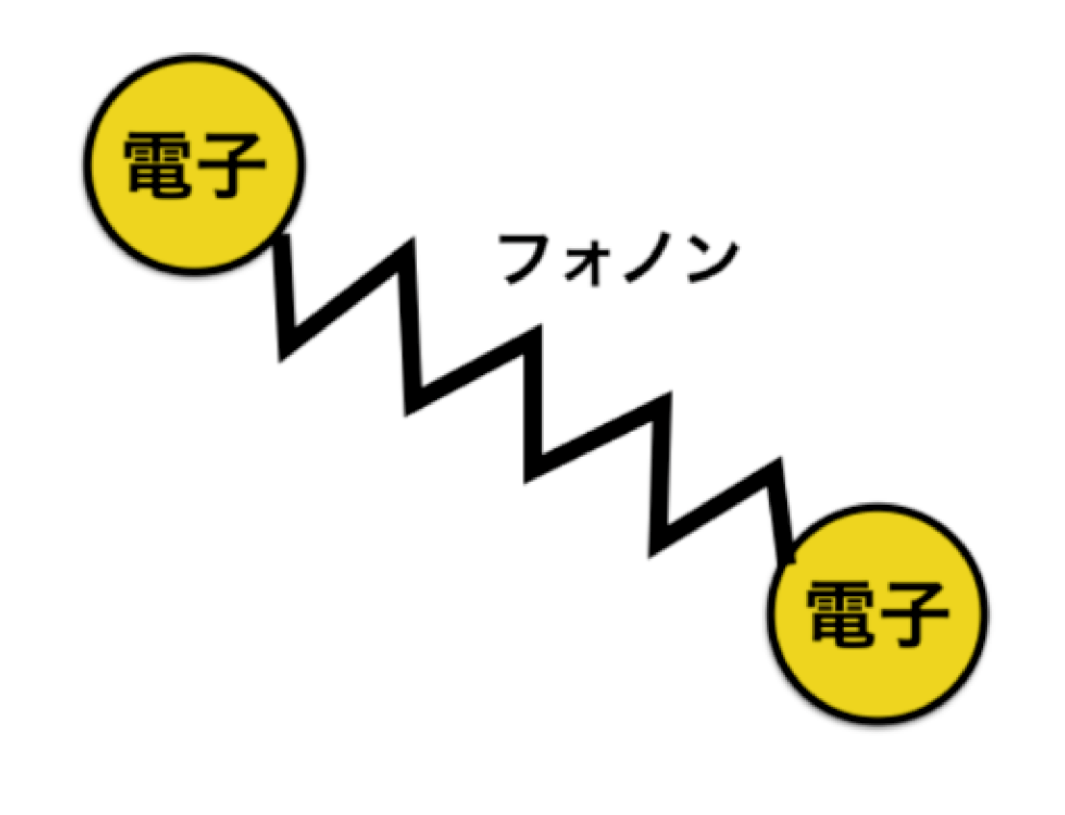
\includegraphics[width=9.0cm]{./Chapter/Chapter2/Picture/Cooperpair.eps}
    \caption{クーパー対概念図}
    \label{fig:CooperPair}
  \end{center}
\end{figure}

またボーズ$\cdot$アインシュタイン凝縮によりフェルミ準位近傍の電子は失われ、エネルギーギャップ$\Delta$が形成される。このエネルギーギャップ$\Delta$の2倍の$2 \Delta$が、クーパー対の結合エネルギーである。エネルギーギャップは超伝導体によって異なり、BCS理論から以下の関係が判明している。
\begin{eqnarray}
2 \Delta = 3.52 k_{B} T_{C}
\label{eq:E_Tc}
\end{eqnarray}
このことから、超伝導転移温度$\mathrm{T_C}$が小さいほど、エネルギーギャップ$\Delta$は小さくなることがわかる。
表\ref{tab:TcDelta}に異なる物質ごとのそれぞれの転移温度$T_C$とエネルギーギャップ$\Delta$を示した。

\begin{table}[htb]
	\begin{center}
		\caption{各物質ごとの転移温度$\mathrm{T_C}$とエネルギーギャップ$\Delta$}
		\begin{tabular}{| l || c | c | c | c |} \hline
			超伝導体 & Si & Nb & Al & Hf \\ \hline \hline
			転移温度$\mathrm{T_C}$[K] & - & 9.23 & 1.20 & 0.165 \\ \hline
			エネルギーギャップ$\Delta$[meV] & 1100 & 1.550 & 0.172 & 0.020 \\ \hline
		\end{tabular}
		\label{tab:TcDelta}
	\end{center}
\end{table}

	
\section{超電導トンネル接合素子光検出器(STJ)}

	\subsection{ジョセフソン効果}
	\begin{figure}[htbp]
  		\begin{center}
    			\includegraphics[width=9.0cm]{./Chapter/Chapter2/Picture/JosephsonJunction.eps}
    			\caption{ジョセフソン接合の概念図}
    			\label{fig:JosephsonJunction}
  		\end{center}
	\end{figure}
	図\ref{fig:JosephsonJunction}のように2つの超伝導体の間に非常に薄い絶縁体を持つSIS(Superconductor / Insulator / Superconductor)構造をもつ素子のことを超伝導トンネル接合素子(Superconducting Tunnel Junction : STJ)と呼ぶ。この素子の絶縁膜をトンネルするトンネル電流には以下の2種類のタイプが存在する。	
	\begin{itemize}
		\item クーパー対のトンネル効果によって流れる超伝導電流
		\item 励起された準粒子のトンネル効果による電流
	\end{itemize}	
	この1つ目の超伝導電流はジョセフソン電流と呼ばれている。このジョセフソン電流には、
	\begin{enumerate}
		\item 直流ジョセフソン電流
		\item 交流ジョセフソン電流
	\end{enumerate}
	の2種類存在する。以下、これらの電流について述べる。
		\subsubsection{直流ジョセフソン電流}
		前述にあるように、ボーズ粒子として振る舞うクーパー対はボーズ・アインシュタイン凝縮し、多数のクーパー対を同時に同一の波動関数、つまり巨視的波動関数で記述することができる。
		そして、図\ref{fig:JosephsonJunction}のような接合において左右の超伝導体でそれぞれ凝縮したクーパー対の系はそれぞれ巨視的波動関数で記述できる。
		ジョセフソン効果には、この位相の差$\delta \theta = \theta_{2} - \theta_{1}$が寄与し、電圧を印加していなくても、
		\begin{eqnarray}
			I = I_{0} \sin (\delta \theta)
			\label{eq:CriticalCurrent}
		\end{eqnarray}
		という超伝導電流が流れる。この$I_{0}$を臨界電流と呼ぶ。
		臨界電流以下なら接合の両端の位相差により、式(\ref{eq:CriticalCurrent})に従って電流が流れる。逆に$I_{0}$以下の電流を流すと式(\ref{eq:CriticalCurrent})に従った位相差が生じる。これを直流ジョセフソン電流という。
		\subsubsection{交流ジョセフソン電流}
		ジョセフソン接合における2つの超伝導体について、クーパー対がトンネルすることを考慮して波動方程式を立てると以下のようになる。
		\begin{eqnarray}
			i \hbar \frac{\partial \Psi_{1}}{\partial t} & = & \mu_{1} \Psi_{1} + K \Psi_{2} \\
			i \hbar \frac{\partial \Psi_{2}}{\partial t} & = & \mu_{2} \Psi_{2} + K \Psi_{1}
			\label{eq:ACJosephson}
		\end{eqnarray}
		
		これを平面解を仮定して解くと、以下のようになる。
		\begin{eqnarray}
			\hbar \frac{\partial n_1}{\partial t} = - \hbar \frac{\partial n_2}{\partial t} = 2 K {n_1}^{1/2} {n_2}^{1/2} \sin (\theta_2 - \theta_1) \\
			- \hbar \frac{\partial}{\partial t} (\theta_2 - \theta_1) = \mu_2 - \mu_1
			\label{eq:ACJosephson_phase}
		\end{eqnarray}
		$K$は2つの超伝導体の結合の強さを示し、$\mu_1$や$\mu_2$はそれぞれの超伝導体におけるクーパー対の化学ポテンシャル、$n_1$や$n_2$はそれぞれの超伝導体でのクーパー対の数密度である。ジョセフソン接合の両端に電位差$V$を与えたとき、接合の両端の位相差は式(\ref{eq:ACJosephson_phase})に従う。
		\begin{eqnarray}
		- \hbar \frac{\partial}{\partial t} \delta \theta = 2eV
		\label{eq:ACJosephson_phase_time}
		\end{eqnarray}
		式(\ref{eq:ACJosephson_phase_time})のように接合両端での位置エネルギー2eVに比例して位相差は時間発展する。このため接合には式(\ref{eq:ACJosephson})のような交流電流が流れる。
		\begin{eqnarray}
			I(t) = I_{0} \sin { \theta (0) - \frac{2eV}{\hbar} t }
			\label{eq:ACJosephson}
		\end{eqnarray}
		このとき周波数は式(\ref{eq:ACJosephson_fre})のようになる。
		\begin{eqnarray}
			2 \pi f = \frac{2eV}{h}
			\label{eq:ACJosephson_fre}
		\end{eqnarray}
		このように、直流電圧を印加することにより、交流電流が発生する現象のことを交流ジョセフソン効果といい、この交流電流のことを交流ジョセフソン電流と呼ぶ。そして、生じる交流の周波数は、$f = 483597.9 \mathrm{GHz/V}$で与えられ、この値をジョセフソン定数と呼ぶ。
	
	\subsection{STJ検出器の構造}
		\begin{figure}[htbp]
  			\begin{center}
    				\includegraphics[width=9.0cm]{./Chapter/Chapter2/Picture/STJ_structure.eps}
    				\caption{超伝導トンネル接合素子光検出器(STJ検出器)\ 構造}
    				\label{fig:STJ_structure}
  			\end{center}
		\end{figure}
		STJの構造を図\ref{fig:STJ_structure}に示す。2枚の超伝導体は厚さ数100nm、大きさ数10〜数100$\mathrm{\mu m}$程度でその間を厚さ1nm程度の薄い絶縁体を挟んだSIS構造を持つ。素子の表面は$\mathrm{SiO_2}$の絶縁膜で覆われており、上部と下部の読み取りはコンタクトホールから配線が伸びて信号の読み出しを行う。
	
	\subsection{STJ検出器の動作原理}
		\begin{figure}[htbp]
  			\begin{center}
    				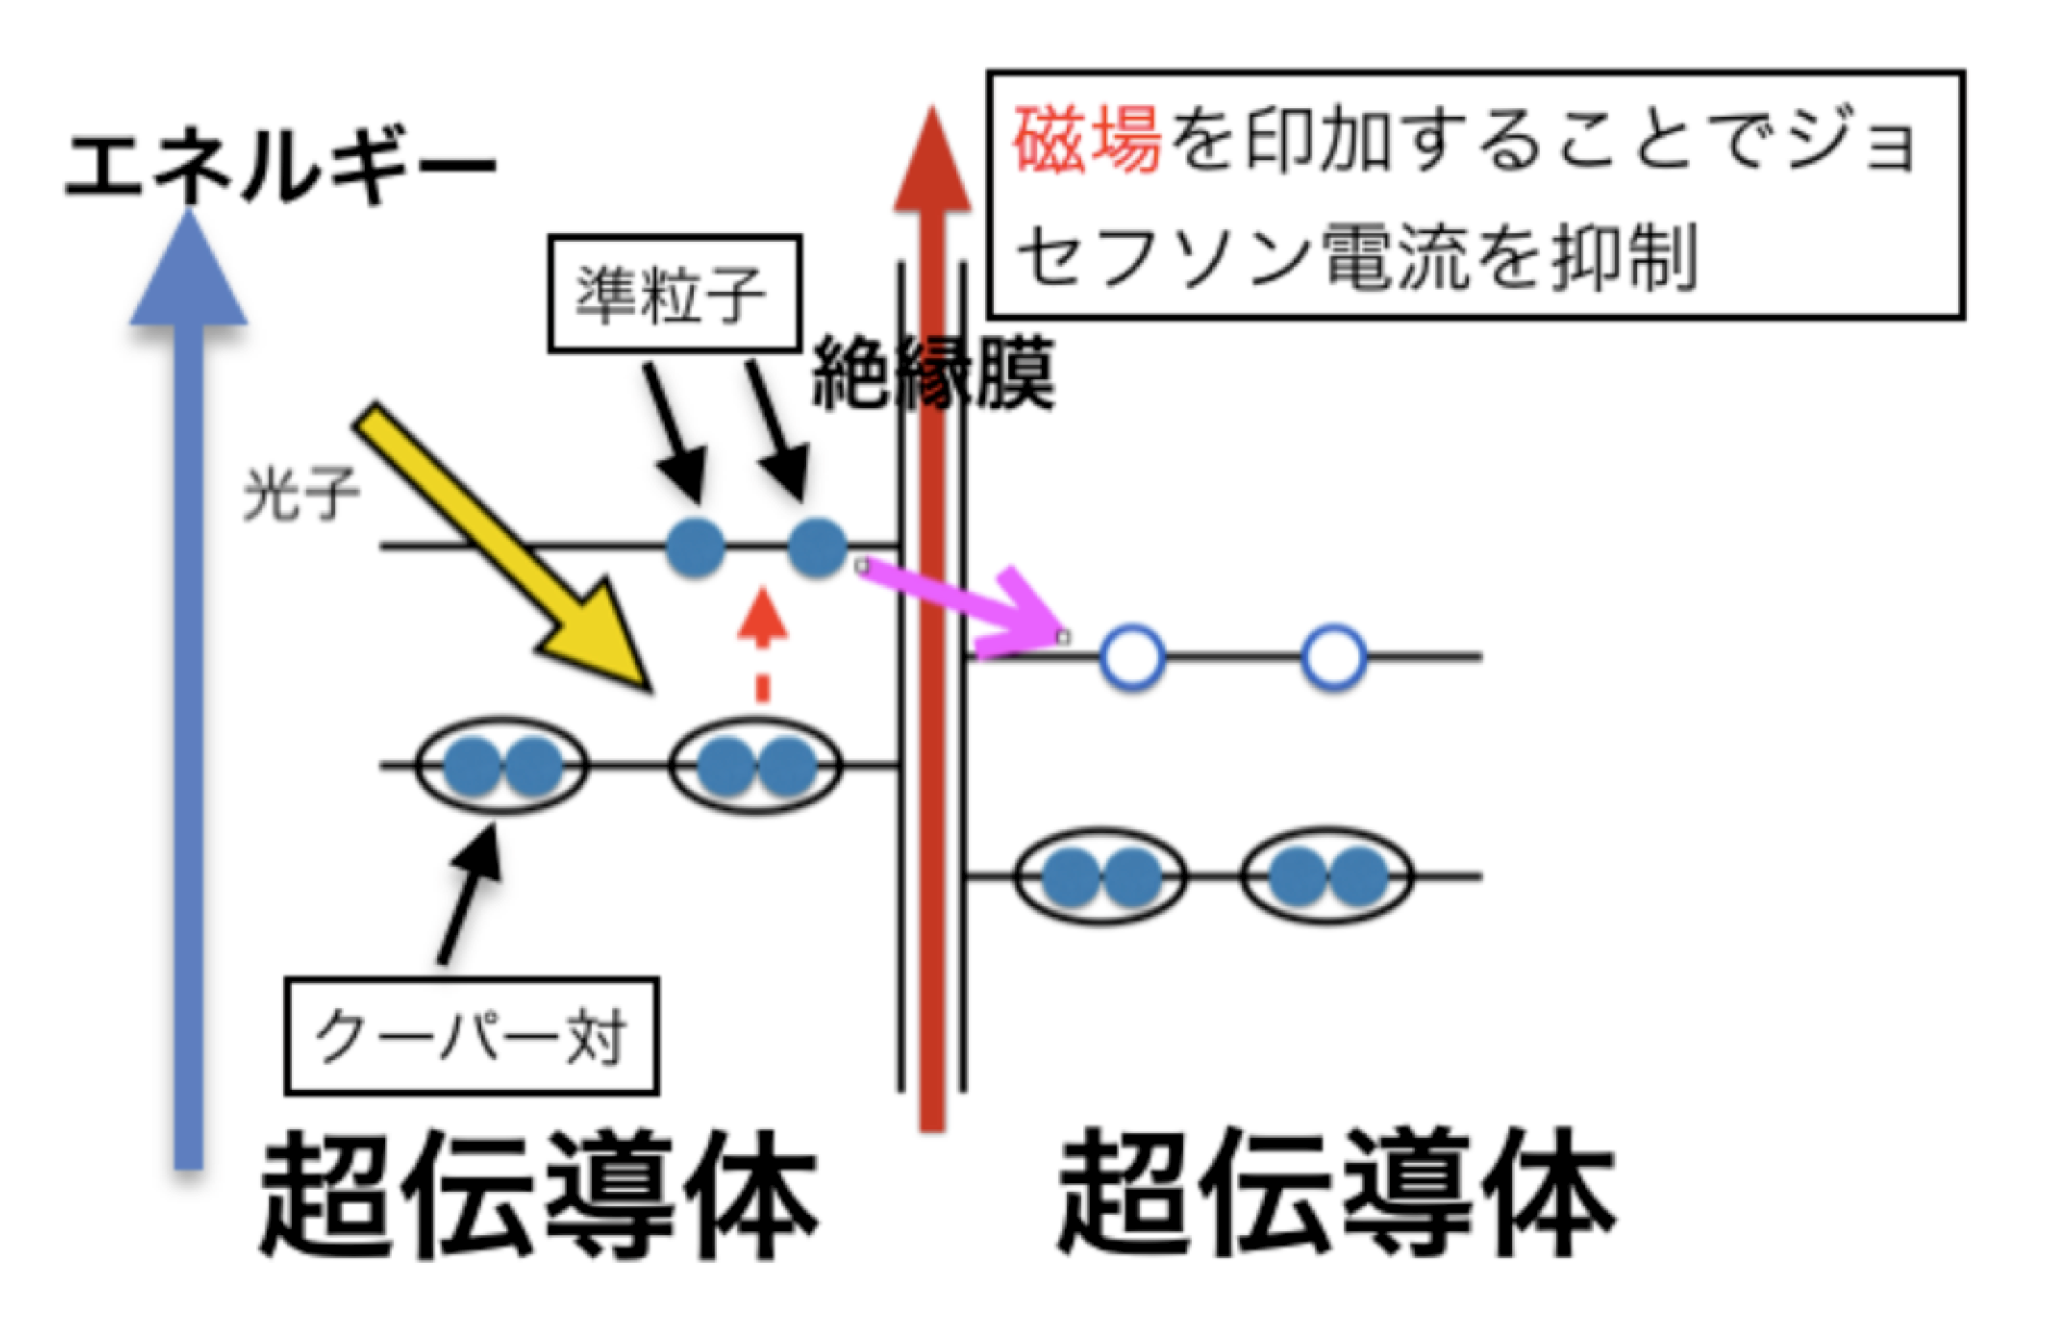
\includegraphics[width=12.0cm]{./Chapter/Chapter2/Picture/STJ_WorkingPrinciple.eps}
    				\caption{超伝導トンネル接合素子光検出器(STJ)動作原理の概念図}
    				\label{fig:STJ_WorkingPrinciple}
  			\end{center}
		\end{figure}
		STJ検出器の動作原理の概念図を図\ref{fig:STJ_WorkingPrinciple}に示す。粒子が検出器中に入射すると、超伝導体中のクーパー対が破壊され準粒子が生成される。生成された準粒子は超伝導体中を拡散し、絶縁膜に到達した準粒子はトンネル効果によって反対側の超伝導体へ通り抜ける。この準粒子のトンネル電流を信号として観測する。STJを動作する際には2つの超伝導体にバイアス電圧を印加し、2つの超伝導体の電位に勾配をつけることで絶縁膜をトンネルした準粒子の逆流を防ぐ。
		
		また、STJ検出器はSIS構造を持つので、信号とは別にジョセフソン電流も生じる。これは信号に対してバックグラウンドになるので抑制する必要がある。このジョセフソン電流は素子の絶縁膜に対して平行に磁場を印加した場合に抑制することができる。ジョセフソン電流$I_C$は磁場が存在すると、フラウンフォーファーと同型の依存性を示す。
		\begin{eqnarray}
			I_{C} = I_{C0} \left| \frac{\sin (\pi \phi / \phi_0)}{\pi \phi / \phi_0} \right|
		\end{eqnarray}
		$\phi$は印加磁場、$\phi_0$は定数である。磁場を印加することでジョセフソン電流が抑制されるので、STJ動作の際には十分な磁場を印加して、微弱な信号を観測する。
	
	\subsection{STJ検出器のエネルギー分解能}
		超伝導体状態ではフェルミオンである電子2つがフォノンを介してクーパー対を形成してボーズ粒子として振る舞う。STJを検出器として動作させる場合、入射粒子が超伝導体中のクーパー対を解離させ、2個の準粒子を生成し、それらの電子がトンネル効果で絶縁膜を通過することが必要になる。STJ信号を得るために必要な最低エネルギーは$2\Delta$である。したがって、$\Delta$が小さければ、それだけエネルギー分解能に優れた検出器ができる。STJのエネルギー分解能は式(\ref{eq:STJ_EnergyResolution})のように表される。
		\begin{eqnarray}
			\sigma_{FWHM} = \frac{\Delta N_q}{N_q} = 2.35 \sqrt{(1.7 \delta) FE}
			\label{eq:STJ_EnergyResolution}
		\end{eqnarray}
		ただし、
		\[
		\begin{cases}
			F : \mathrm{Fano\ Factor} \\
			E : \mathrm{入射粒子のエネルギー}
		\end{cases}
		\]
		である。Nb/Al-STJ検出器の場合、Fano\ Factorは0.1〜0.2程度である。式(\ref{eq:E_Tc})の関係式と照らし合わせて考察する。
		
		STJ検出器開発において、より高いエネルギー分解能が要求されるのに対し、エネルギー分解能を上げるためにエネルギーギャップが小さい超伝導体を用いようとすると、式(\ref{eq:E_Tc})から分かるように転移温度が低くなるので、より低温の測定系構築が要求されることになる。
		
	\subsection{STJのリーク電流}
		磁場を印加している場合、理想的なSTJ検出器ならば接合間に電流が流れることない。しかし、実際には以下で述べるような要因によるリーク電流が存在してしまい、これがSTJ信号のバックグラウンドとなる。
		\subsubsection{不完全な構造的な欠陥}
			酸化膜に開いた微小なピンホールや素子側面での2枚の超伝導体の接触などによるリーク電流をさす。図\ref{fig:STJ_leak_structure}にSTJ検出器の不完全な構造から生じるリーク電流の概念図を載せた。
			\begin{figure}[htbp]
  				\begin{center}
    					\includegraphics[width=12.0cm]{./Chapter/Chapter2/Picture/STJ_leak_structure.eps}
    					\caption{STJ検出器の不完全な構造起因の概念図}
    					\label{fig:STJ_leak_structure}
  				\end{center}
			\end{figure}	
		
		\subsubsection{熱励起によって生じる準粒子}
		構造的な欠陥をいくら改善しても、有限温度であれば必ず熱励起によって生じる準粒子は存在する。その準粒子がトンネル効果によって絶縁膜を流れるのならば、それはリーク電流となり得る。このリーク電流の温度依存性は理論的に計算されており、リーク電流$I_{\mathrm{leak}}$と温度$T$との関係は式(\ref{eq:STJ_leak_temp})のように書ける。\cite{13}
		\begin{eqnarray}
			I_{\mathrm{leak}} \propto T^{1/2} \exp \left(- \frac{\Delta}{k_{B}T} \right)
			\label{eq:STJ_leak_temp}
		\end{eqnarray}
		この式から、熱起因によるリーク電流は温度が下がるにつれて指数関数的に減少する。つまり、ここから言えることはSTJ検出器で十分なパフォーマンスを発揮するためには構造的な欠陥を極力抑えることに加えて、十分に冷却する必要もある。
		
		\subsubsection{その他}	
	
	\subsection{STJ検出器の電流電圧特性}
		\begin{figure}[htbp]
  			\begin{center}
    				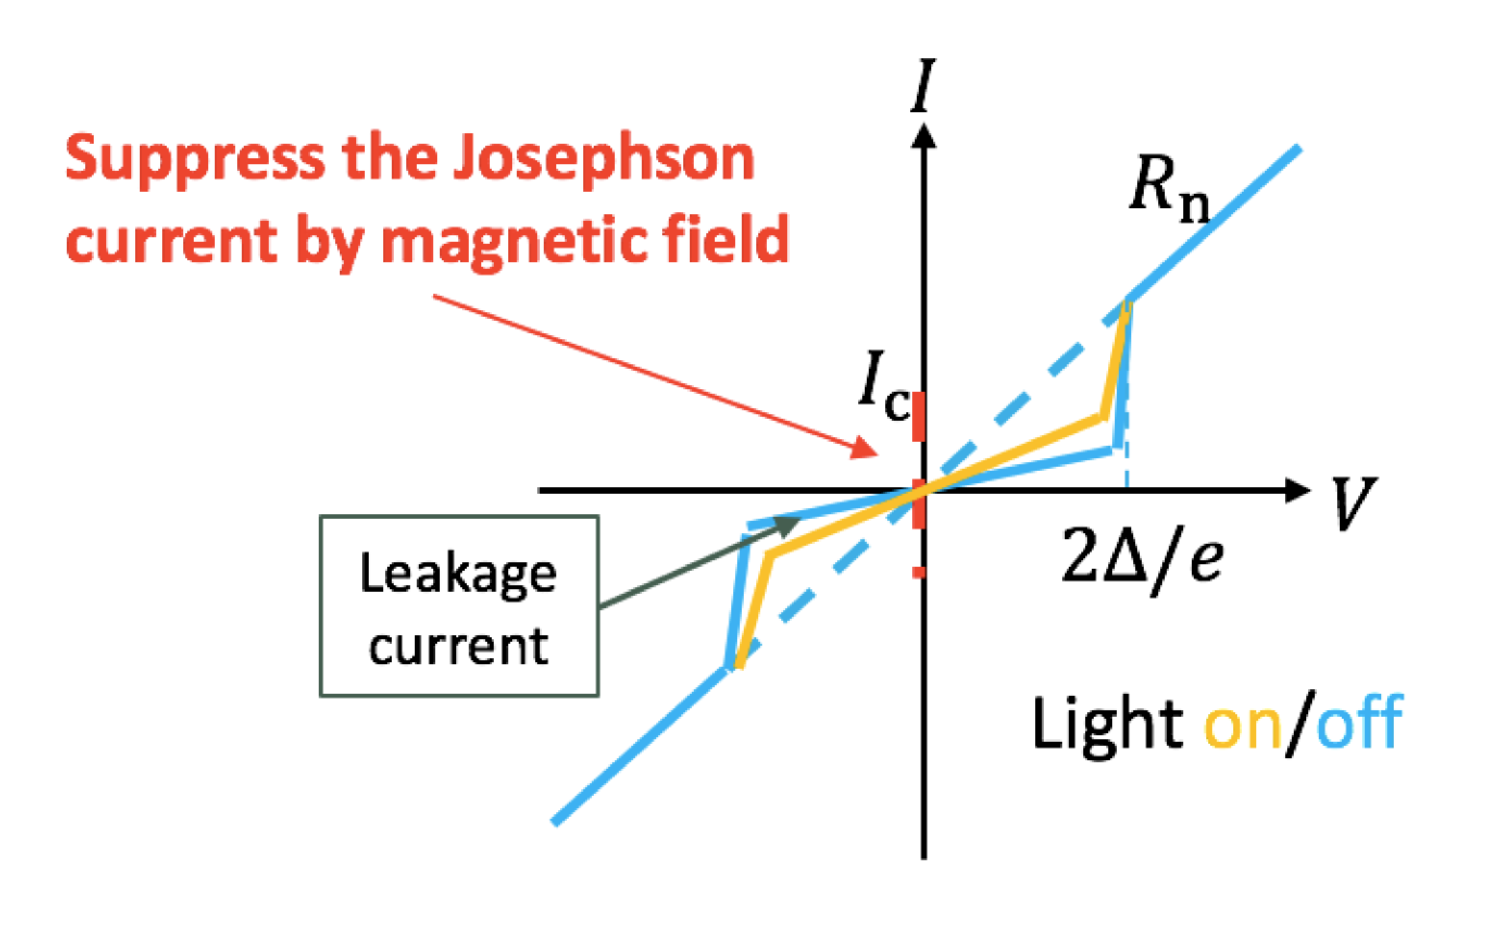
\includegraphics[width=12.0cm]{./Chapter/Chapter2/Picture/STJ_IV.eps}
    				\caption{一般的なSTJ検出器の電流電圧特性}
	  			\label{fig:STJ_IV}
  			\end{center}
		\end{figure}
		STJ検出器の電流電圧特性を図\ref{fig:STJ_IV}に示す。このSTJ検出器の電流電圧特性を測定し、素子の性能評価を行う。
		\begin{description}
			\item[$0 < |V| < 2 \Delta / e$の場合]\mbox{}\\
				クーパー対は準粒子として絶縁膜をトンネルすることができず、理想的には電流は流れない。しかし、前述したように不完全な構造や熱などに起因するリーク電流が存在するために、実際は電流はゼロにならず、有限の抵抗を持つ。この領域のことは「ダイナミックレジスタンス領域」と呼ばれ、そしてこの領域での抵抗値は$R_d$と表される。
			\item[$|V| > 2 \Delta /e$の場合]\mbox{}\\
				クーパー対はもう一方の超伝導体へトンネルすることができる。したがって、この領域での電流電圧特性は通常の抵抗のように振る舞う。この領域のことは「ノーマルレジスタンス領域」と呼ばれ、そしてこの領域での抵抗値は$R_n$と表される。
		\end{description}
		
		したがって、通常のSTJ検出器として動作させる場合は、印加電圧Vが「ダイナミックレジスタンス領域」に収まるように設定する。またSTJ検出器に光が入射した場合、クーパー対解離によって生じるトンネル電流が増加するので、図\ref{fig:STJ_IV}のように、青線から黄線に変化する。
	
\section{Nb/Al-STJ検出器}
	我々はニュートリノ崩壊光探索実験に用いるSTJ検出器として、超伝導体にハフニウムHfを用いた「Hf-STJ」と、超伝導体にニオブNbとアルミニウムAlを組み合わせた「Nb/Al-STJ」の研究開発を行っている。
	Hf-STJは、用いる超伝導体ハフニウムHfのエネルギーギャップ$\Delta$が0.020meVと非常に小さいのでエネルギー分解能に非常に優れている。我々は2012年に世界初のハフニウムHfを用いたHf-STJ検出器の作製に成功し、光に対する応答を確認した。このHf-STJは品質の良い素子作製プロセスを確立するために現在研究開発の最中である。また、これは将来の衛星実験の際に用いることを考えている。
	本節では、Hf-STJではなく、衛星実験の前実験であるロケット実験に用いるNb/Al-STJについて述べる。
	\subsection{Nb/Al-STJ検出器の構造}
		\begin{figure}[htbp]
  			\begin{center}
    				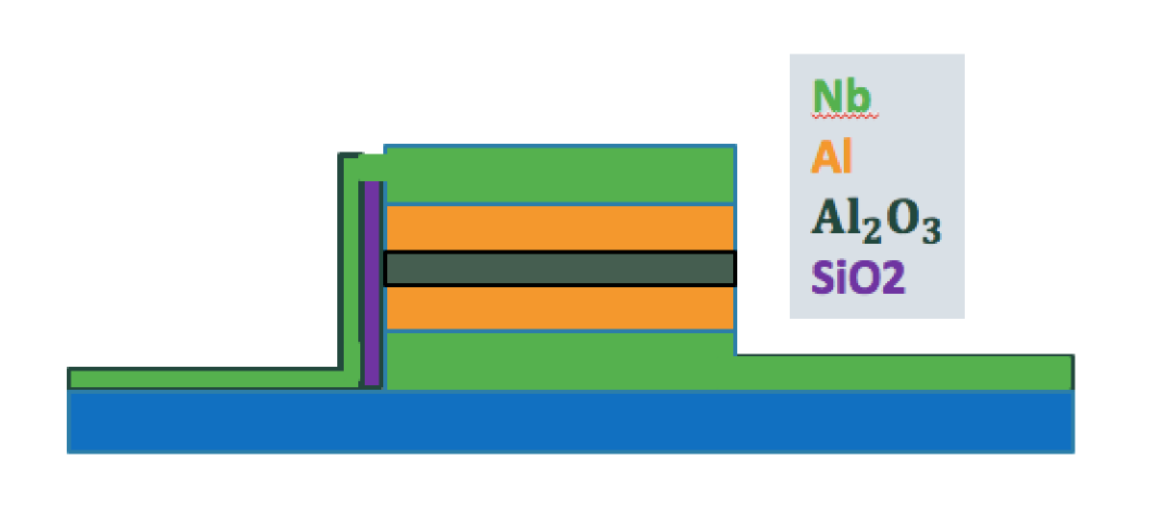
\includegraphics[width=12.0cm]{./Chapter/Chapter2/Picture/NbAlSTJ_structure.eps}
    				\caption{Nb/Al-STJ検出器の構造概念図}
	  			\label{fig:NbAlSTJ_structure}
  			\end{center}
		\end{figure}
		前述したように、Nb/Al-STJ検出器はニュートリノ崩壊光探索ロケット実験に用いる予定で、現在研究開発中である。用いる超伝導体に、ニオブNbとアルミニウムAlの2種類の超伝導体を組み合わせており、絶縁膜に酸化アルミニウム$\mathrm{Al_{2}O_3}$を用いている。Nb/Al-STJ検出器の構造を図\ref{fig:NbAlSTJ_structure}に示す。
		ニオブNb層と絶縁膜の間に、ニオブNbのエネルギーギャップ$\Delta_{\mathrm{Nb}}$に比べて更にエネルギーギャップが小さいアルミニウムAl層を挟むことによって、STJ検出器として動作させる際に有利に働く以下の特徴が現れる。
		\begin{description}
			\item[より高品質な絶縁膜の形成]\mbox{}\\
				Nb酸化膜を絶縁膜としたSTJ検出器は熱サイクルに弱く、繰り返し冷却して使用できない。一方、Al酸化膜は熱サイクルに強い。\\
				使い勝手のよいSTJ検出器を作製するために、Al酸化膜をNb系STJ検出器に用いる場合、必然的にニオブNb層とAl酸化膜の間にAl層を形成することになる。
			\item[近接効果による転移温度$T_C$とエネルギーギャップ$\Delta$の調節]\mbox{}\\
				ニオブの転移温度$T_{C\mathrm{Nb}}$が9.2Kであるのに対し、アルミニウムの転移温度$T_{C\mathrm{Al}}$は1.1Kと低い。
				2つの超伝導体を接合した場合、一方の超伝導体のクーパー対の波動関数がもう一方の超伝導体内に染み出し、転移温度が変化する。
				この効果を「近接効果」という。変化の度合いは2つの超伝導体の厚みの比率に応じて変化する。
				式(\ref{eq:E_Tc})と照らし合わせて考えると、Al層の厚さを調節することによって、転移温度と、同時にエネルギーギャップ$\Delta$を調節することができる。
				したがって、Al層を挟むことによって、Nb単体で作製されたSTJ検出器に比べてエネルギーギャップ$\Delta$は下がる。
				結果エネルギー分解能を向上させることが可能である。
			\item[バックトンネリングによるトンネル準粒子数の増加]\mbox{}\\
				\begin{figure}[htbp]
  					\begin{center}
    						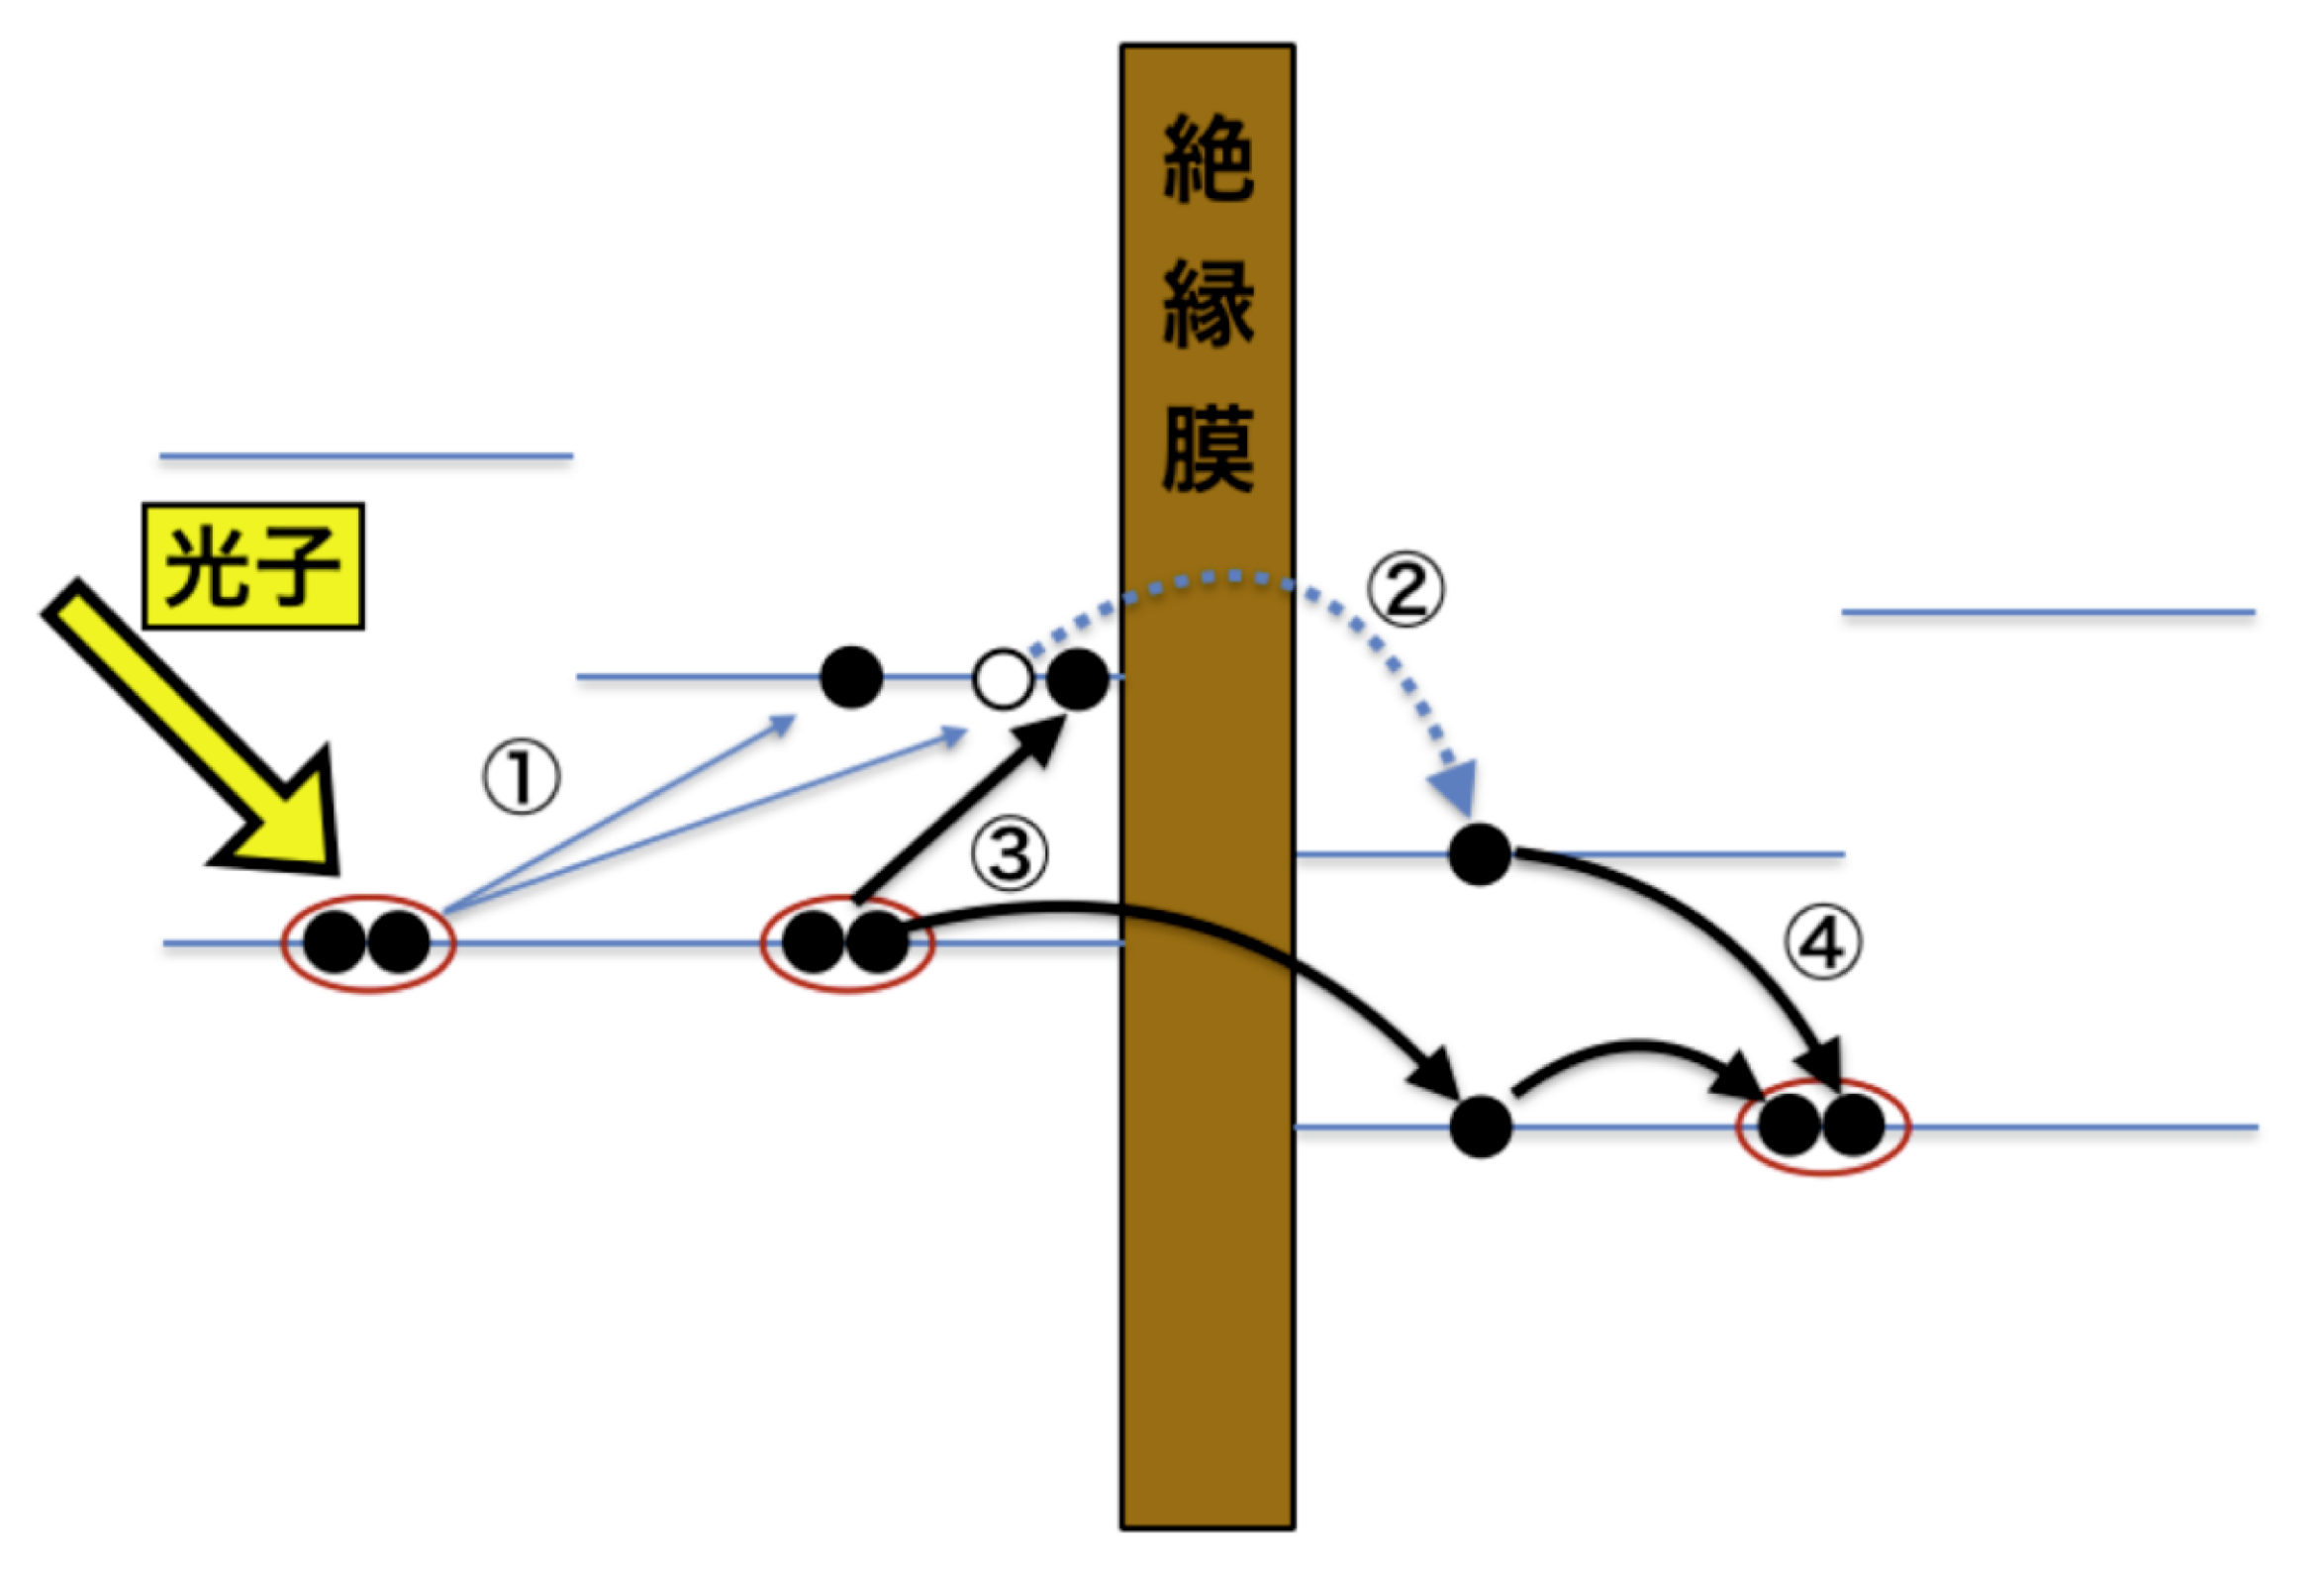
\includegraphics[width=12.0cm]{./Chapter/Chapter2/Picture/NbAlSTJ_backtunnel.eps}
    						\caption{バックトンネリング効果の概念図}
	  					\label{fig:NbAlSTJ_backtunnel}
  					\end{center}
				\end{figure}
				Nb/Al-STJ検出器のように、超伝導体と絶縁膜の間によりエネルギーギャップが小さい超伝導体を挟むことでトンネルする準粒子数が増加する、バックトンネリング効果が現れる。図\ref{fig:NbAlSTJ_backtunnel}にバックトンネリング効果の概念図を載せる。
				
				バックトンネリング効果の流れは以下のようになる。
				\begin{enumerate}
					\item STJ検出器の上部伝導体に入射した粒子がクーパー対を壊し、2つの準粒子を発生させる。
					\item 2つの準粒子のうち、1つは上部超伝導体のAl層の常伝導体にトラップされて、もう1つは絶縁膜をトンネルして下部聴伝導体のAl層の常伝導体にトラップされる。
					\item 下部超伝導体にクーパー対を作ろうと、上部伝導体の別のクーパー対が壊されて新たに2つの準粒子が生成される。
					\item 先に絶縁膜をトンネルした粒子どうしが再結合してクーパー対をなす。
					\item 残された準粒子は上部超伝導体のAl層常伝導体でトラップされる
				\end{enumerate}
				この一連の流れを繰り返すことでトンネル準粒子数が増加、つまりトンネル電流が増加する。
				バックトンネリング効果を踏まえ、STJ検出器にエネルギーEを持つ粒子が入射したときの準粒子生成個数$N$は、
				\begin{eqnarray}
					N = G_{\mathrm{Al}} \frac{E}{1.7 \Delta}
				\end{eqnarray}
				となる。この$G_{\mathrm{Al}}$をトラッピングゲインと呼び、バックトンネリング効果によるトンネル準粒子数の増加率を表す。トラッピングゲイン$G_{\mathrm{Al}}$は約10倍程度とされている。
		\end{description}

	\subsection{Nb/Al-STJ検出器の研究開発の現状}
		本研究グループは2014年度から、産業技術総合研究所(AIST)との共同研究を開始した。
		そして、Nb/Al-STJ検出器素子作製は産業技術総合研究所のCRAVITY(Clean Room for Analog-digital superconductiVITY)で行なわれている。
		ここでは安定して高品質の超伝導素子を作製することができる。
		
		図\ref{fig:NbAlSTJ_leaktemp}にCRAVITYで作製されたNb/Al-STJ検出器のリーク電流の温度依存性を示す。
		素子のサイズは$50 \times 50 \mathrm{{\mu m}^2}$である。
		この図からわかるように、0.4K程度以下でリーク電流が飽和することがわかる。この飽和したリーク電流は熱起因ではないリーク電流であり、より高品質のSTJ検出器素子作製や測定系の改善を行うことで下げることができる。
		25meVの一光子をリーク電流の揺らぎに対して$3 \sigma$以上で検出するためには、STJ検出器の信号幅を$1 \mathrm{\mu s}$と仮定すると、STJ検出器のリーク電流要求値は100pA以下である必要がある。
		表\ref{tab:NbAlSTJ_leaksize}に、我々が測定したNb/Al-STJ検出器のサイズごとのリーク電流値を示す。この表からCRAVITY製のNb/Al-STJ検出器はCOBAND実験のリーク電流の要求値を満たしていることがわかる。
		
		しかし、現在もなおNb/Al-STJ検出器を用いて遠赤外光一光子検出の成功には至っていない。その理由として、STJ検出器からの信号を冷凍機外部へと長い配線を経て読み出す際に、測定系由来の雑音がSTJ検出器信号に大きく効いてきてしまうからだ。この問題の解決策として、STJ検出器が動作する極低温環境下においても動作可能な前置増幅器を冷凍機内に設置し、STJ検出器信号が雑音に埋もれてしまう前に増幅する方法がある。\\
		我々は現在、この極低温前置増幅器の研究開発を行なっており、次章はこれについて詳しく述べる。
		%=====Nb/Al-STJのリーク電流温度依存性のplotを載せる=====%
		\begin{figure}[htbp]
  			\begin{center}
  				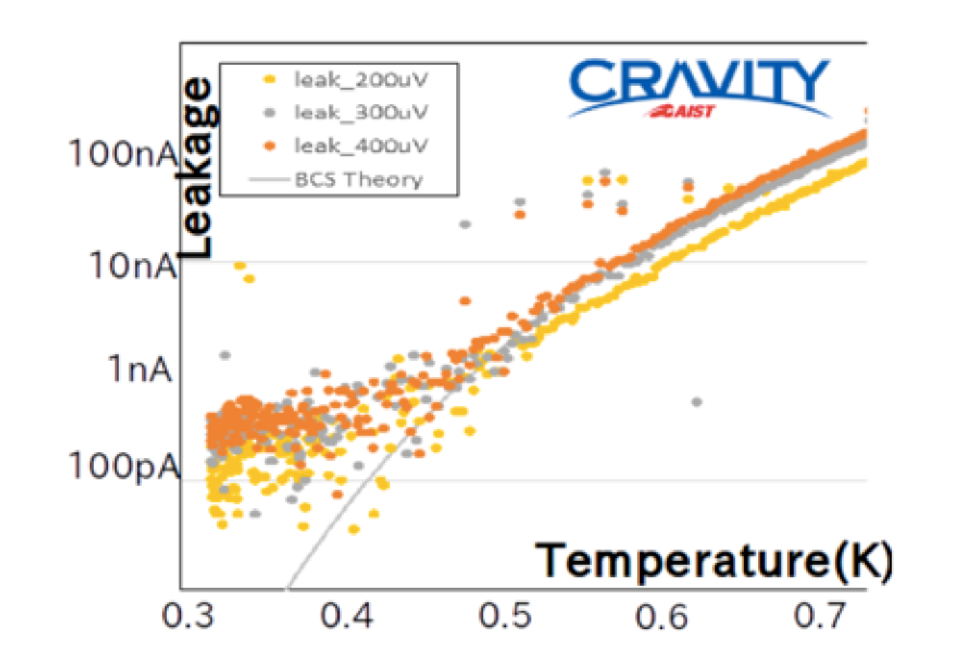
\includegraphics[width=8.0cm]{./Chapter/Chapter2/Picture/NbAlSTJ_leaktemp.eps}
    				\caption{CRAVITY製Nb/Al-STJ検出器のリーク電流温度依存性}
	  			\label{fig:NbAlSTJ_leaktemp}
 			\end{center}
		\end{figure}
		%=====現在のリーク電流の状況を表にして載せる=====%
		\begin{table}[htb]
			\begin{center}
				\caption{CRAVITY製Nb/Al-STJ検出器のサイズごとのリーク電流値}
				\begin{tabular}{| l || c | c | c |} \hline
					Nb/Al-STJのサイズ & ${100 \mathrm{\mu m}}^2$ & ${50 \mathrm{\mu m}}^2$ & ${20 \mathrm{\mu m}}^2$ \\ \hline
					リーク電流$I_{\mathrm{leak}}$@0.4mV & 2 nA & 300 pA & 100 pA \\ \hline
				\end{tabular}
				\label{tab:NbAlSTJ_leaksize}
			\end{center}
		\end{table}




%%%%%%%%%%%%%%%%%%%%%%%%%%%%%%%%%%%%%%%%%%%%%%%%%%%%%%%%%%%%%%%
\chapter{超伝導トンネル接合素子光検出器(STJ)}
前章で述べたように、ニュートリノ崩壊から放出される光子のエネルギーは25meVであると予想されている。したがって用いる検出器への要求は、
\begin{enumerate}
\item 25meVのエネルギー領域で感度を持つこと
\item エネルギースペクトルからニュートリノ崩壊光として評価するためにはエネルギー分解能$2 \%$を達成すること
\end{enumerate}
が必要である。

一方、検出器のエネルギー分解能はその物質のエネルギーギャップによって決まるが、通常の半導体検出器では前述した要求を満たさず、検出器開発は不可能であると考えられる。
したがって、我々は上記の要求を達成するために、ニュートリノ崩壊光探索実験において、超伝導トンネル接合素子光検出器(STJ : Superconducting Tunnel Junction、以下「STJ」と表記する)を用いる。STJとは、非常に薄い絶縁膜を2つの超伝導体で挟んだ構造をしており、超伝導体の転移温度以下で動作可能な検出器である。半導体に比べて非常にエネルギーギャップが小さいので、目標のエネルギー分解能を達成することができると考え、研究開発を進めている。
本章では、STJについて説明し、我々が研究開発しているNb/Al-STJ検出器開発について述べる。
\section{超伝導の基礎}
超伝導体の示す基本的な実験事実として、「完全電気伝導性」と「完全反磁性」の2つを述べる。
	\begin{description}
	\item[完全電気伝導性]\mbox{}\\
		1911年、オランダのH.Kamerlingh Onnesは水銀を液体ヘリウムで冷却して行った時、温度4.2Kで突然電気抵抗が下がり、4.19Kで$10^{-5} \Omega$以下になる現象を報告した。その後、水銀以外にも特定の金属や合金に対し、温度を下げていくと突然急激に電気抵抗が下がりほぼ0になる性質を持つことが発見された。このように電気抵抗が急激に落ちて0になる超伝導体特有の性質を「完全電気伝導性」と呼び、そしてこの時の温度のことを臨界温度(critical temperature)、または転移温度(transition temperature)といい、$\mathrm{T_C}$と表す。
	\item[完全反磁性]\mbox{}\\
		1933年にF.Walther Meissnerによって超伝導体に完全反磁性を示すことが発見された。この効果をMeissner効果と呼び、超伝導体内部では磁場が排除される。
	\end{description}
	
超伝導現象の基礎になる理論は1957年にJ.Bardeen、L. N. Cooper、J. M. Schriefferによって発見され、この理論のことを頭文字をとって、「BCS理論」という。この理論では、臨界温度$\mathrm{T_C}$以下の温度において電子$\cdot$格子相互作用を介して電子対のスピンが互いに逆向き、対の角運動量の合計がゼロの状態が形成され、これらの電子同士に引力が働くと考えられている。BCS理論では図\ref{fig:CooperPair}のように電子$\cdot$格子相互作用を介して電子同士がフォノンを仮想的に交換することによって引力が働くと考える。その引力によって結合している電子対のことをクーパー対(cooper pair)と呼ぶ。電子$\cdot$電子対のクーパー対は運動量、スピンがゼロのボーズ粒子として振る舞い、ボーズ$\cdot$アインシュタイン凝縮を起こし1つの量子状態へ落ち込む。多数のクーパー対が同じ状態に落ち込むということは、つまり多数のクーパー対を同時に同一の波動関数で記述できる。この波動関数を巨視的波動関数という。

\begin{eqnarray}
\Phi (\bm{r},t) = |\Phi (\bm{r},t)| \exp (i \theta (\bm{r},t))
\end{eqnarray}

\begin{figure}[htbp]
  \begin{center}
    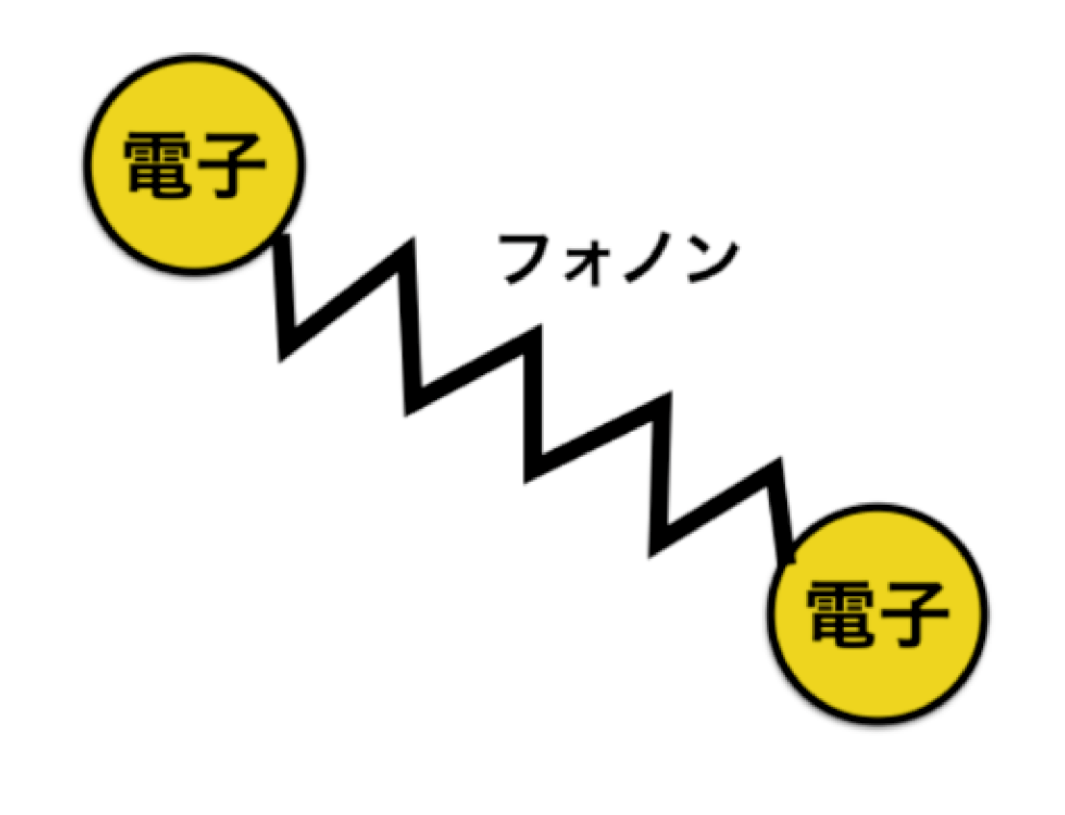
\includegraphics[width=9.0cm]{./Chapter/Chapter2/Picture/Cooperpair.eps}
    \caption{クーパー対概念図}
    \label{fig:CooperPair}
  \end{center}
\end{figure}

またボーズ$\cdot$アインシュタイン凝縮によりフェルミ準位近傍の電子は失われ、エネルギーギャップ$\Delta$が形成される。このエネルギーギャップ$\Delta$の2倍の$2 \Delta$が、クーパー対の結合エネルギーである。エネルギーギャップは超伝導体によって異なり、BCS理論から以下の関係が判明している。
\begin{eqnarray}
2 \Delta = 3.52 k_{B} T_{C}
\label{eq:E_Tc}
\end{eqnarray}
このことから、超伝導転移温度$\mathrm{T_C}$が小さいほど、エネルギーギャップ$\Delta$は小さくなることがわかる。
表\ref{tab:TcDelta}に異なる物質ごとのそれぞれの転移温度$T_C$とエネルギーギャップ$\Delta$を示した。

\begin{table}[htb]
	\begin{center}
		\caption{各物質ごとの転移温度$\mathrm{T_C}$とエネルギーギャップ$\Delta$}
		\begin{tabular}{| l || c | c | c | c |} \hline
			超伝導体 & Si & Nb & Al & Hf \\ \hline \hline
			転移温度$\mathrm{T_C}$[K] & - & 9.23 & 1.20 & 0.165 \\ \hline
			エネルギーギャップ$\Delta$[meV] & 1100 & 1.550 & 0.172 & 0.020 \\ \hline
		\end{tabular}
		\label{tab:TcDelta}
	\end{center}
\end{table}

	
\section{超電導トンネル接合素子光検出器(STJ)}

	\subsection{ジョセフソン効果}
	\begin{figure}[htbp]
  		\begin{center}
    			\includegraphics[width=9.0cm]{./Chapter/Chapter2/Picture/JosephsonJunction.eps}
    			\caption{ジョセフソン接合の概念図}
    			\label{fig:JosephsonJunction}
  		\end{center}
	\end{figure}
	図\ref{fig:JosephsonJunction}のように2つの超伝導体の間に非常に薄い絶縁体を持つSIS(Superconductor / Insulator / Superconductor)構造をもつ素子のことを超伝導トンネル接合素子(Superconducting Tunnel Junction : STJ)と呼ぶ。この素子の絶縁膜をトンネルするトンネル電流には以下の2種類のタイプが存在する。	
	\begin{itemize}
		\item クーパー対のトンネル効果によって流れる超伝導電流
		\item 励起された準粒子のトンネル効果による電流
	\end{itemize}	
	この1つ目の超伝導電流はジョセフソン電流と呼ばれている。このジョセフソン電流には、
	\begin{enumerate}
		\item 直流ジョセフソン電流
		\item 交流ジョセフソン電流
	\end{enumerate}
	の2種類存在する。以下、これらの電流について述べる。
		\subsubsection{直流ジョセフソン電流}
		前述にあるように、ボーズ粒子として振る舞うクーパー対はボーズ・アインシュタイン凝縮し、多数のクーパー対を同時に同一の波動関数、つまり巨視的波動関数で記述することができる。
		そして、図\ref{fig:JosephsonJunction}のような接合において左右の超伝導体でそれぞれ凝縮したクーパー対の系はそれぞれ巨視的波動関数で記述できる。
		ジョセフソン効果には、この位相の差$\delta \theta = \theta_{2} - \theta_{1}$が寄与し、電圧を印加していなくても、
		\begin{eqnarray}
			I = I_{0} \sin (\delta \theta)
			\label{eq:CriticalCurrent}
		\end{eqnarray}
		という超伝導電流が流れる。この$I_{0}$を臨界電流と呼ぶ。
		臨界電流以下なら接合の両端の位相差により、式(\ref{eq:CriticalCurrent})に従って電流が流れる。逆に$I_{0}$以下の電流を流すと式(\ref{eq:CriticalCurrent})に従った位相差が生じる。これを直流ジョセフソン電流という。
		\subsubsection{交流ジョセフソン電流}
		ジョセフソン接合における2つの超伝導体について、クーパー対がトンネルすることを考慮して波動方程式を立てると以下のようになる。
		\begin{eqnarray}
			i \hbar \frac{\partial \Psi_{1}}{\partial t} & = & \mu_{1} \Psi_{1} + K \Psi_{2} \\
			i \hbar \frac{\partial \Psi_{2}}{\partial t} & = & \mu_{2} \Psi_{2} + K \Psi_{1}
			\label{eq:ACJosephson}
		\end{eqnarray}
		
		これを平面解を仮定して解くと、以下のようになる。
		\begin{eqnarray}
			\hbar \frac{\partial n_1}{\partial t} = - \hbar \frac{\partial n_2}{\partial t} = 2 K {n_1}^{1/2} {n_2}^{1/2} \sin (\theta_2 - \theta_1) \\
			- \hbar \frac{\partial}{\partial t} (\theta_2 - \theta_1) = \mu_2 - \mu_1
			\label{eq:ACJosephson_phase}
		\end{eqnarray}
		$K$は2つの超伝導体の結合の強さを示し、$\mu_1$や$\mu_2$はそれぞれの超伝導体におけるクーパー対の化学ポテンシャル、$n_1$や$n_2$はそれぞれの超伝導体でのクーパー対の数密度である。ジョセフソン接合の両端に電位差$V$を与えたとき、接合の両端の位相差は式(\ref{eq:ACJosephson_phase})に従う。
		\begin{eqnarray}
		- \hbar \frac{\partial}{\partial t} \delta \theta = 2eV
		\label{eq:ACJosephson_phase_time}
		\end{eqnarray}
		式(\ref{eq:ACJosephson_phase_time})のように接合両端での位置エネルギー2eVに比例して位相差は時間発展する。このため接合には式(\ref{eq:ACJosephson})のような交流電流が流れる。
		\begin{eqnarray}
			I(t) = I_{0} \sin { \theta (0) - \frac{2eV}{\hbar} t }
			\label{eq:ACJosephson}
		\end{eqnarray}
		このとき周波数は式(\ref{eq:ACJosephson_fre})のようになる。
		\begin{eqnarray}
			2 \pi f = \frac{2eV}{h}
			\label{eq:ACJosephson_fre}
		\end{eqnarray}
		このように、直流電圧を印加することにより、交流電流が発生する現象のことを交流ジョセフソン効果といい、この交流電流のことを交流ジョセフソン電流と呼ぶ。そして、生じる交流の周波数は、$f = 483597.9 \mathrm{GHz/V}$で与えられ、この値をジョセフソン定数と呼ぶ。
	
	\subsection{STJ検出器の構造}
		\begin{figure}[htbp]
  			\begin{center}
    				\includegraphics[width=9.0cm]{./Chapter/Chapter2/Picture/STJ_structure.eps}
    				\caption{超伝導トンネル接合素子光検出器(STJ検出器)\ 構造}
    				\label{fig:STJ_structure}
  			\end{center}
		\end{figure}
		STJの構造を図\ref{fig:STJ_structure}に示す。2枚の超伝導体は厚さ数100nm、大きさ数10〜数100$\mathrm{\mu m}$程度でその間を厚さ1nm程度の薄い絶縁体を挟んだSIS構造を持つ。素子の表面は$\mathrm{SiO_2}$の絶縁膜で覆われており、上部と下部の読み取りはコンタクトホールから配線が伸びて信号の読み出しを行う。
	
	\subsection{STJ検出器の動作原理}
		\begin{figure}[htbp]
  			\begin{center}
    				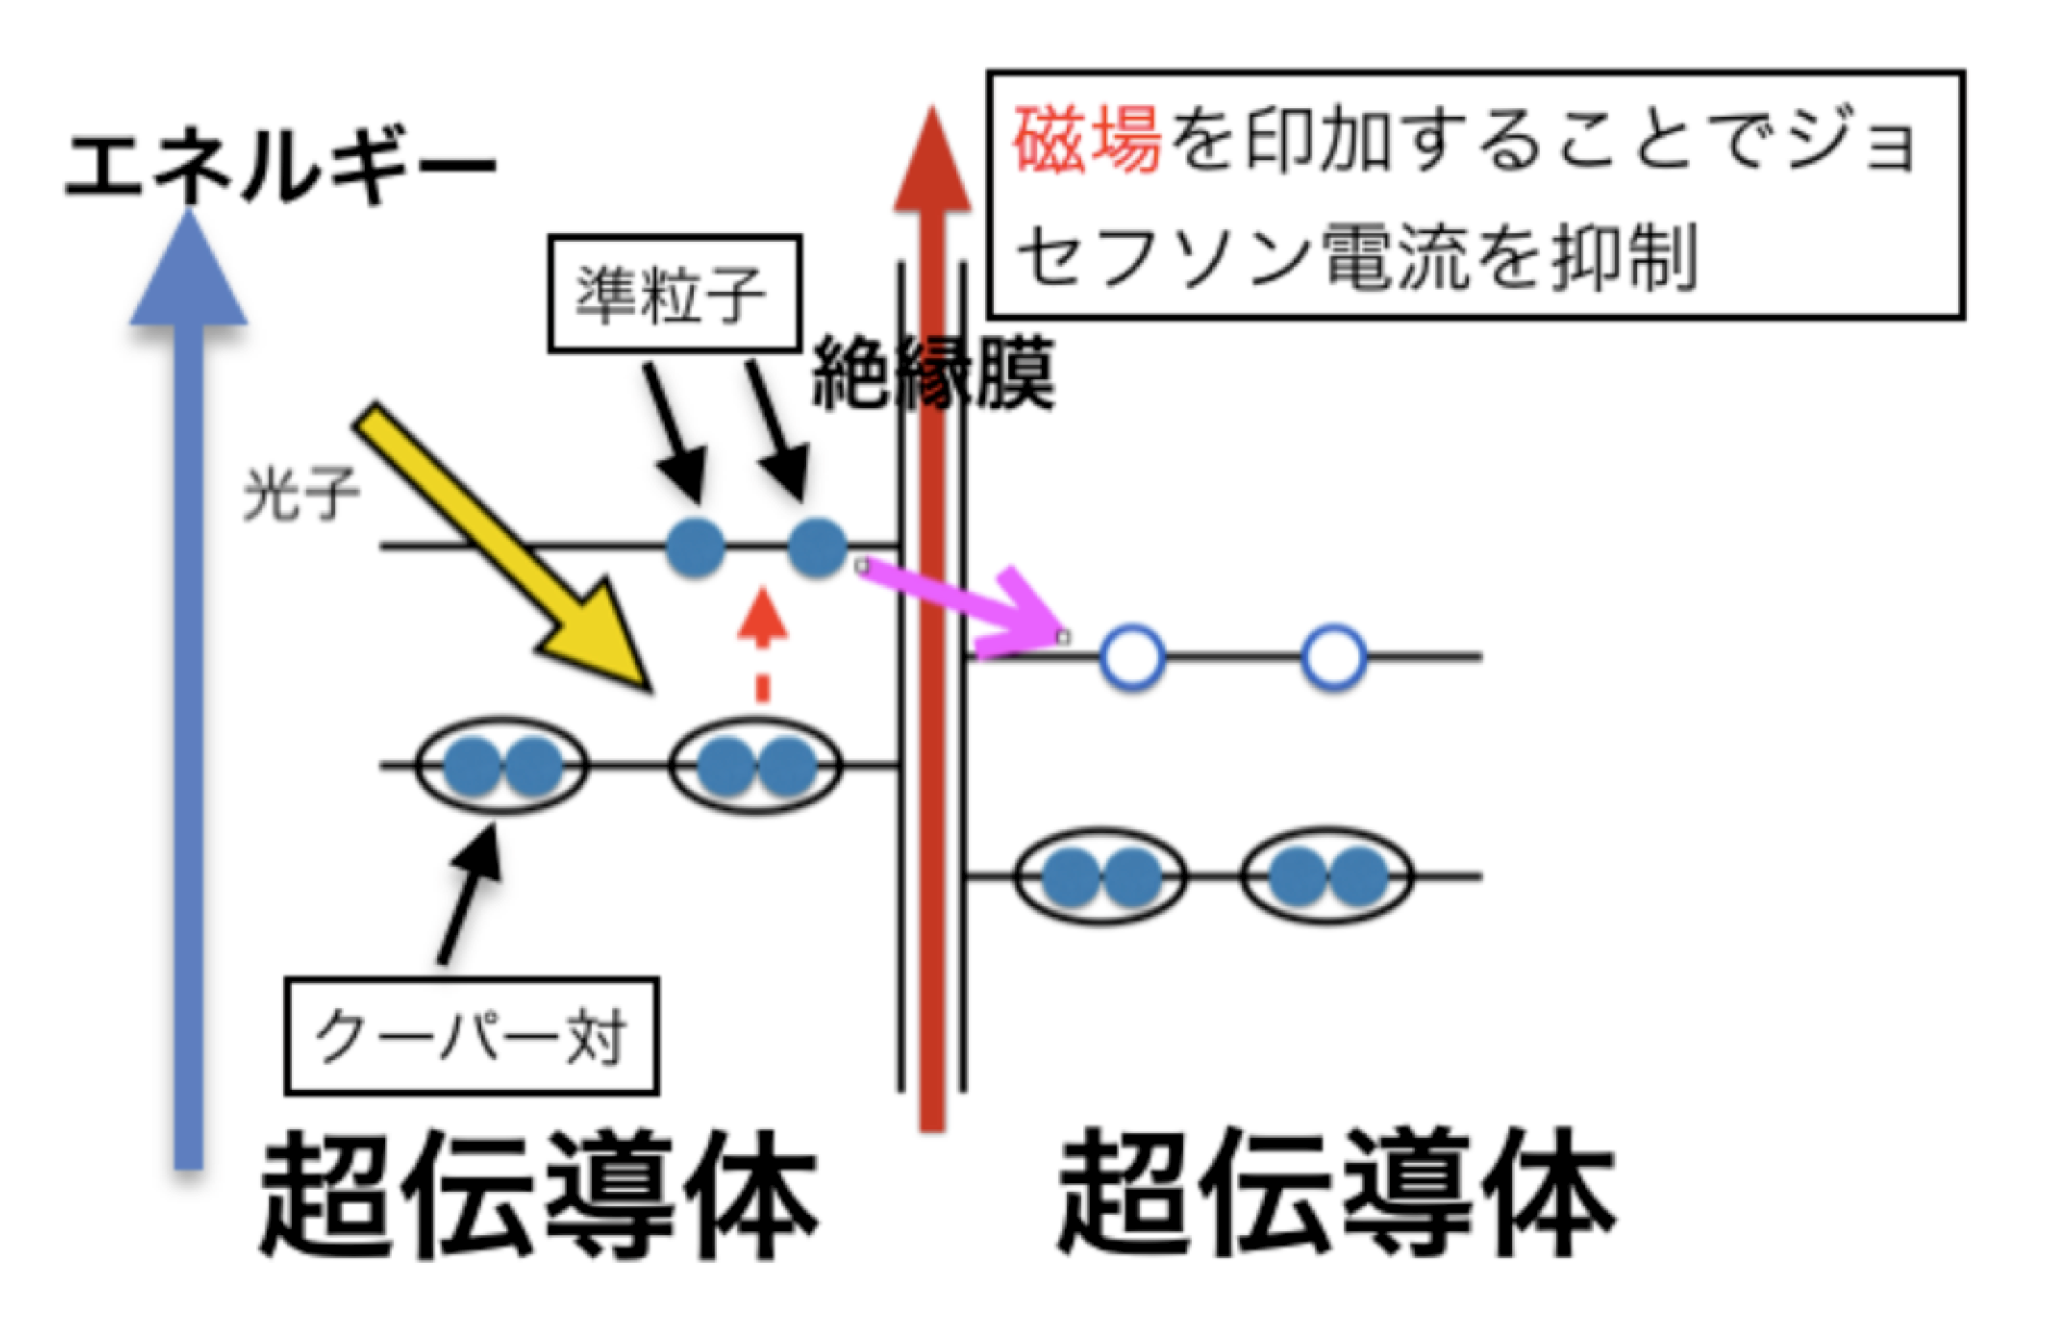
\includegraphics[width=12.0cm]{./Chapter/Chapter2/Picture/STJ_WorkingPrinciple.eps}
    				\caption{超伝導トンネル接合素子光検出器(STJ)動作原理の概念図}
    				\label{fig:STJ_WorkingPrinciple}
  			\end{center}
		\end{figure}
		STJ検出器の動作原理の概念図を図\ref{fig:STJ_WorkingPrinciple}に示す。粒子が検出器中に入射すると、超伝導体中のクーパー対が破壊され準粒子が生成される。生成された準粒子は超伝導体中を拡散し、絶縁膜に到達した準粒子はトンネル効果によって反対側の超伝導体へ通り抜ける。この準粒子のトンネル電流を信号として観測する。STJを動作する際には2つの超伝導体にバイアス電圧を印加し、2つの超伝導体の電位に勾配をつけることで絶縁膜をトンネルした準粒子の逆流を防ぐ。
		
		また、STJ検出器はSIS構造を持つので、信号とは別にジョセフソン電流も生じる。これは信号に対してバックグラウンドになるので抑制する必要がある。このジョセフソン電流は素子の絶縁膜に対して平行に磁場を印加した場合に抑制することができる。ジョセフソン電流$I_C$は磁場が存在すると、フラウンフォーファーと同型の依存性を示す。
		\begin{eqnarray}
			I_{C} = I_{C0} \left| \frac{\sin (\pi \phi / \phi_0)}{\pi \phi / \phi_0} \right|
		\end{eqnarray}
		$\phi$は印加磁場、$\phi_0$は定数である。磁場を印加することでジョセフソン電流が抑制されるので、STJ動作の際には十分な磁場を印加して、微弱な信号を観測する。
	
	\subsection{STJ検出器のエネルギー分解能}
		超伝導体状態ではフェルミオンである電子2つがフォノンを介してクーパー対を形成してボーズ粒子として振る舞う。STJを検出器として動作させる場合、入射粒子が超伝導体中のクーパー対を解離させ、2個の準粒子を生成し、それらの電子がトンネル効果で絶縁膜を通過することが必要になる。STJ信号を得るために必要な最低エネルギーは$2\Delta$である。したがって、$\Delta$が小さければ、それだけエネルギー分解能に優れた検出器ができる。STJのエネルギー分解能は式(\ref{eq:STJ_EnergyResolution})のように表される。
		\begin{eqnarray}
			\sigma_{FWHM} = \frac{\Delta N_q}{N_q} = 2.35 \sqrt{(1.7 \delta) FE}
			\label{eq:STJ_EnergyResolution}
		\end{eqnarray}
		ただし、
		\[
		\begin{cases}
			F : \mathrm{Fano\ Factor} \\
			E : \mathrm{入射粒子のエネルギー}
		\end{cases}
		\]
		である。Nb/Al-STJ検出器の場合、Fano\ Factorは0.1〜0.2程度である。式(\ref{eq:E_Tc})の関係式と照らし合わせて考察する。
		
		STJ検出器開発において、より高いエネルギー分解能が要求されるのに対し、エネルギー分解能を上げるためにエネルギーギャップが小さい超伝導体を用いようとすると、式(\ref{eq:E_Tc})から分かるように転移温度が低くなるので、より低温の測定系構築が要求されることになる。
		
	\subsection{STJのリーク電流}
		磁場を印加している場合、理想的なSTJ検出器ならば接合間に電流が流れることない。しかし、実際には以下で述べるような要因によるリーク電流が存在してしまい、これがSTJ信号のバックグラウンドとなる。
		\subsubsection{不完全な構造的な欠陥}
			酸化膜に開いた微小なピンホールや素子側面での2枚の超伝導体の接触などによるリーク電流をさす。図\ref{fig:STJ_leak_structure}にSTJ検出器の不完全な構造から生じるリーク電流の概念図を載せた。
			\begin{figure}[htbp]
  				\begin{center}
    					\includegraphics[width=12.0cm]{./Chapter/Chapter2/Picture/STJ_leak_structure.eps}
    					\caption{STJ検出器の不完全な構造起因の概念図}
    					\label{fig:STJ_leak_structure}
  				\end{center}
			\end{figure}	
		
		\subsubsection{熱励起によって生じる準粒子}
		構造的な欠陥をいくら改善しても、有限温度であれば必ず熱励起によって生じる準粒子は存在する。その準粒子がトンネル効果によって絶縁膜を流れるのならば、それはリーク電流となり得る。このリーク電流の温度依存性は理論的に計算されており、リーク電流$I_{\mathrm{leak}}$と温度$T$との関係は式(\ref{eq:STJ_leak_temp})のように書ける。\cite{13}
		\begin{eqnarray}
			I_{\mathrm{leak}} \propto T^{1/2} \exp \left(- \frac{\Delta}{k_{B}T} \right)
			\label{eq:STJ_leak_temp}
		\end{eqnarray}
		この式から、熱起因によるリーク電流は温度が下がるにつれて指数関数的に減少する。つまり、ここから言えることはSTJ検出器で十分なパフォーマンスを発揮するためには構造的な欠陥を極力抑えることに加えて、十分に冷却する必要もある。
		
		\subsubsection{その他}	
	
	\subsection{STJ検出器の電流電圧特性}
		\begin{figure}[htbp]
  			\begin{center}
    				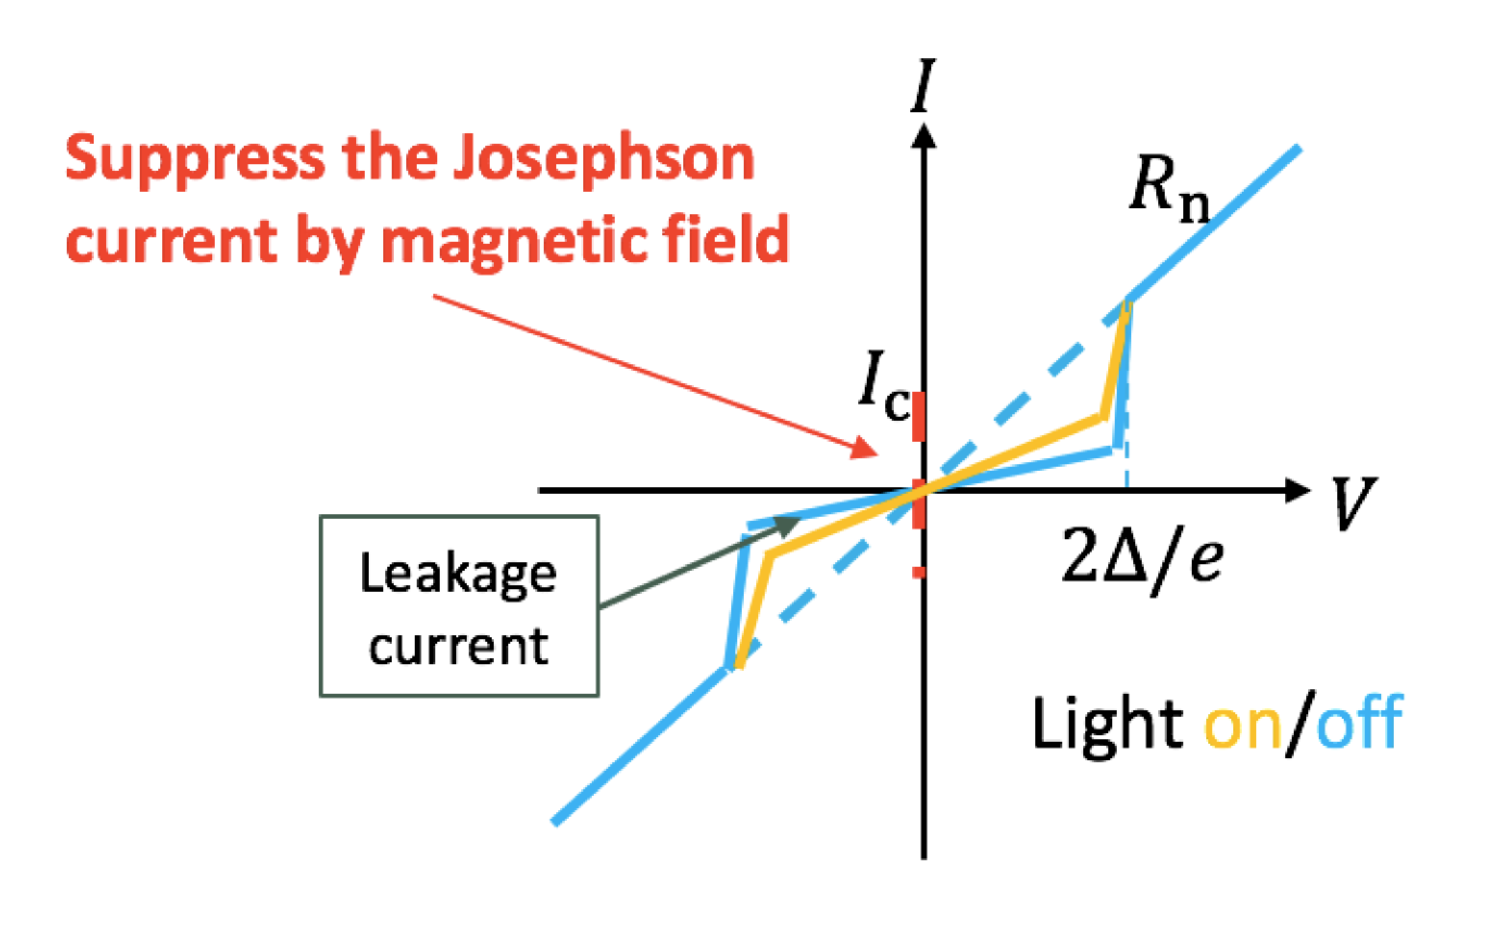
\includegraphics[width=12.0cm]{./Chapter/Chapter2/Picture/STJ_IV.eps}
    				\caption{一般的なSTJ検出器の電流電圧特性}
	  			\label{fig:STJ_IV}
  			\end{center}
		\end{figure}
		STJ検出器の電流電圧特性を図\ref{fig:STJ_IV}に示す。このSTJ検出器の電流電圧特性を測定し、素子の性能評価を行う。
		\begin{description}
			\item[$0 < |V| < 2 \Delta / e$の場合]\mbox{}\\
				クーパー対は準粒子として絶縁膜をトンネルすることができず、理想的には電流は流れない。しかし、前述したように不完全な構造や熱などに起因するリーク電流が存在するために、実際は電流はゼロにならず、有限の抵抗を持つ。この領域のことは「ダイナミックレジスタンス領域」と呼ばれ、そしてこの領域での抵抗値は$R_d$と表される。
			\item[$|V| > 2 \Delta /e$の場合]\mbox{}\\
				クーパー対はもう一方の超伝導体へトンネルすることができる。したがって、この領域での電流電圧特性は通常の抵抗のように振る舞う。この領域のことは「ノーマルレジスタンス領域」と呼ばれ、そしてこの領域での抵抗値は$R_n$と表される。
		\end{description}
		
		したがって、通常のSTJ検出器として動作させる場合は、印加電圧Vが「ダイナミックレジスタンス領域」に収まるように設定する。またSTJ検出器に光が入射した場合、クーパー対解離によって生じるトンネル電流が増加するので、図\ref{fig:STJ_IV}のように、青線から黄線に変化する。
	
\section{Nb/Al-STJ検出器}
	我々はニュートリノ崩壊光探索実験に用いるSTJ検出器として、超伝導体にハフニウムHfを用いた「Hf-STJ」と、超伝導体にニオブNbとアルミニウムAlを組み合わせた「Nb/Al-STJ」の研究開発を行っている。
	Hf-STJは、用いる超伝導体ハフニウムHfのエネルギーギャップ$\Delta$が0.020meVと非常に小さいのでエネルギー分解能に非常に優れている。我々は2012年に世界初のハフニウムHfを用いたHf-STJ検出器の作製に成功し、光に対する応答を確認した。このHf-STJは品質の良い素子作製プロセスを確立するために現在研究開発の最中である。また、これは将来の衛星実験の際に用いることを考えている。
	本節では、Hf-STJではなく、衛星実験の前実験であるロケット実験に用いるNb/Al-STJについて述べる。
	\subsection{Nb/Al-STJ検出器の構造}
		\begin{figure}[htbp]
  			\begin{center}
    				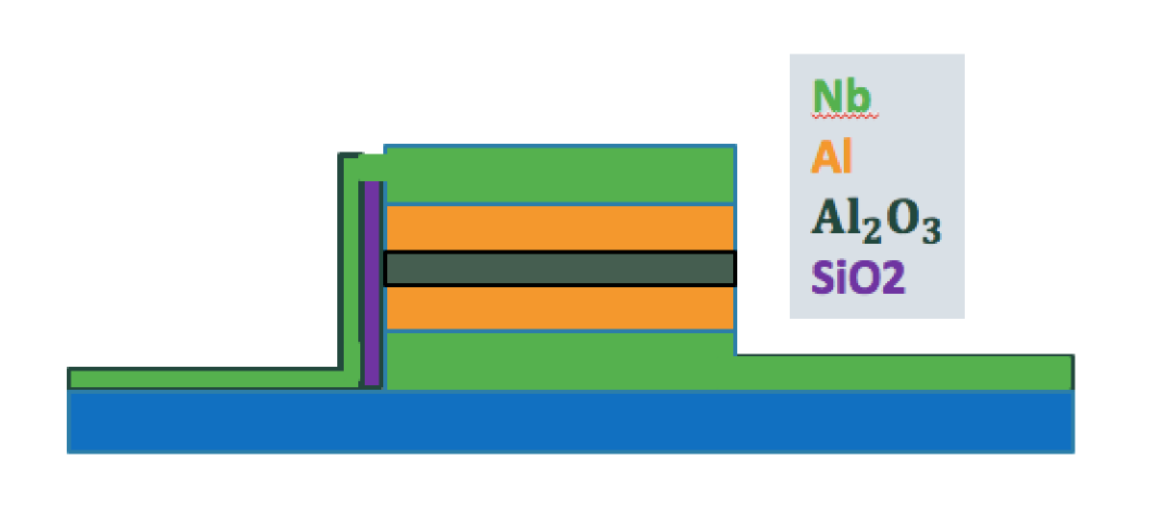
\includegraphics[width=12.0cm]{./Chapter/Chapter2/Picture/NbAlSTJ_structure.eps}
    				\caption{Nb/Al-STJ検出器の構造概念図}
	  			\label{fig:NbAlSTJ_structure}
  			\end{center}
		\end{figure}
		前述したように、Nb/Al-STJ検出器はニュートリノ崩壊光探索ロケット実験に用いる予定で、現在研究開発中である。用いる超伝導体に、ニオブNbとアルミニウムAlの2種類の超伝導体を組み合わせており、絶縁膜に酸化アルミニウム$\mathrm{Al_{2}O_3}$を用いている。Nb/Al-STJ検出器の構造を図\ref{fig:NbAlSTJ_structure}に示す。
		ニオブNb層と絶縁膜の間に、ニオブNbのエネルギーギャップ$\Delta_{\mathrm{Nb}}$に比べて更にエネルギーギャップが小さいアルミニウムAl層を挟むことによって、STJ検出器として動作させる際に有利に働く以下の特徴が現れる。
		\begin{description}
			\item[より高品質な絶縁膜の形成]\mbox{}\\
				Nb酸化膜を絶縁膜としたSTJ検出器は熱サイクルに弱く、繰り返し冷却して使用できない。一方、Al酸化膜は熱サイクルに強い。\\
				使い勝手のよいSTJ検出器を作製するために、Al酸化膜をNb系STJ検出器に用いる場合、必然的にニオブNb層とAl酸化膜の間にAl層を形成することになる。
			\item[近接効果による転移温度$T_C$とエネルギーギャップ$\Delta$の調節]\mbox{}\\
				ニオブの転移温度$T_{C\mathrm{Nb}}$が9.2Kであるのに対し、アルミニウムの転移温度$T_{C\mathrm{Al}}$は1.1Kと低い。
				2つの超伝導体を接合した場合、一方の超伝導体のクーパー対の波動関数がもう一方の超伝導体内に染み出し、転移温度が変化する。
				この効果を「近接効果」という。変化の度合いは2つの超伝導体の厚みの比率に応じて変化する。
				式(\ref{eq:E_Tc})と照らし合わせて考えると、Al層の厚さを調節することによって、転移温度と、同時にエネルギーギャップ$\Delta$を調節することができる。
				したがって、Al層を挟むことによって、Nb単体で作製されたSTJ検出器に比べてエネルギーギャップ$\Delta$は下がる。
				結果エネルギー分解能を向上させることが可能である。
			\item[バックトンネリングによるトンネル準粒子数の増加]\mbox{}\\
				\begin{figure}[htbp]
  					\begin{center}
    						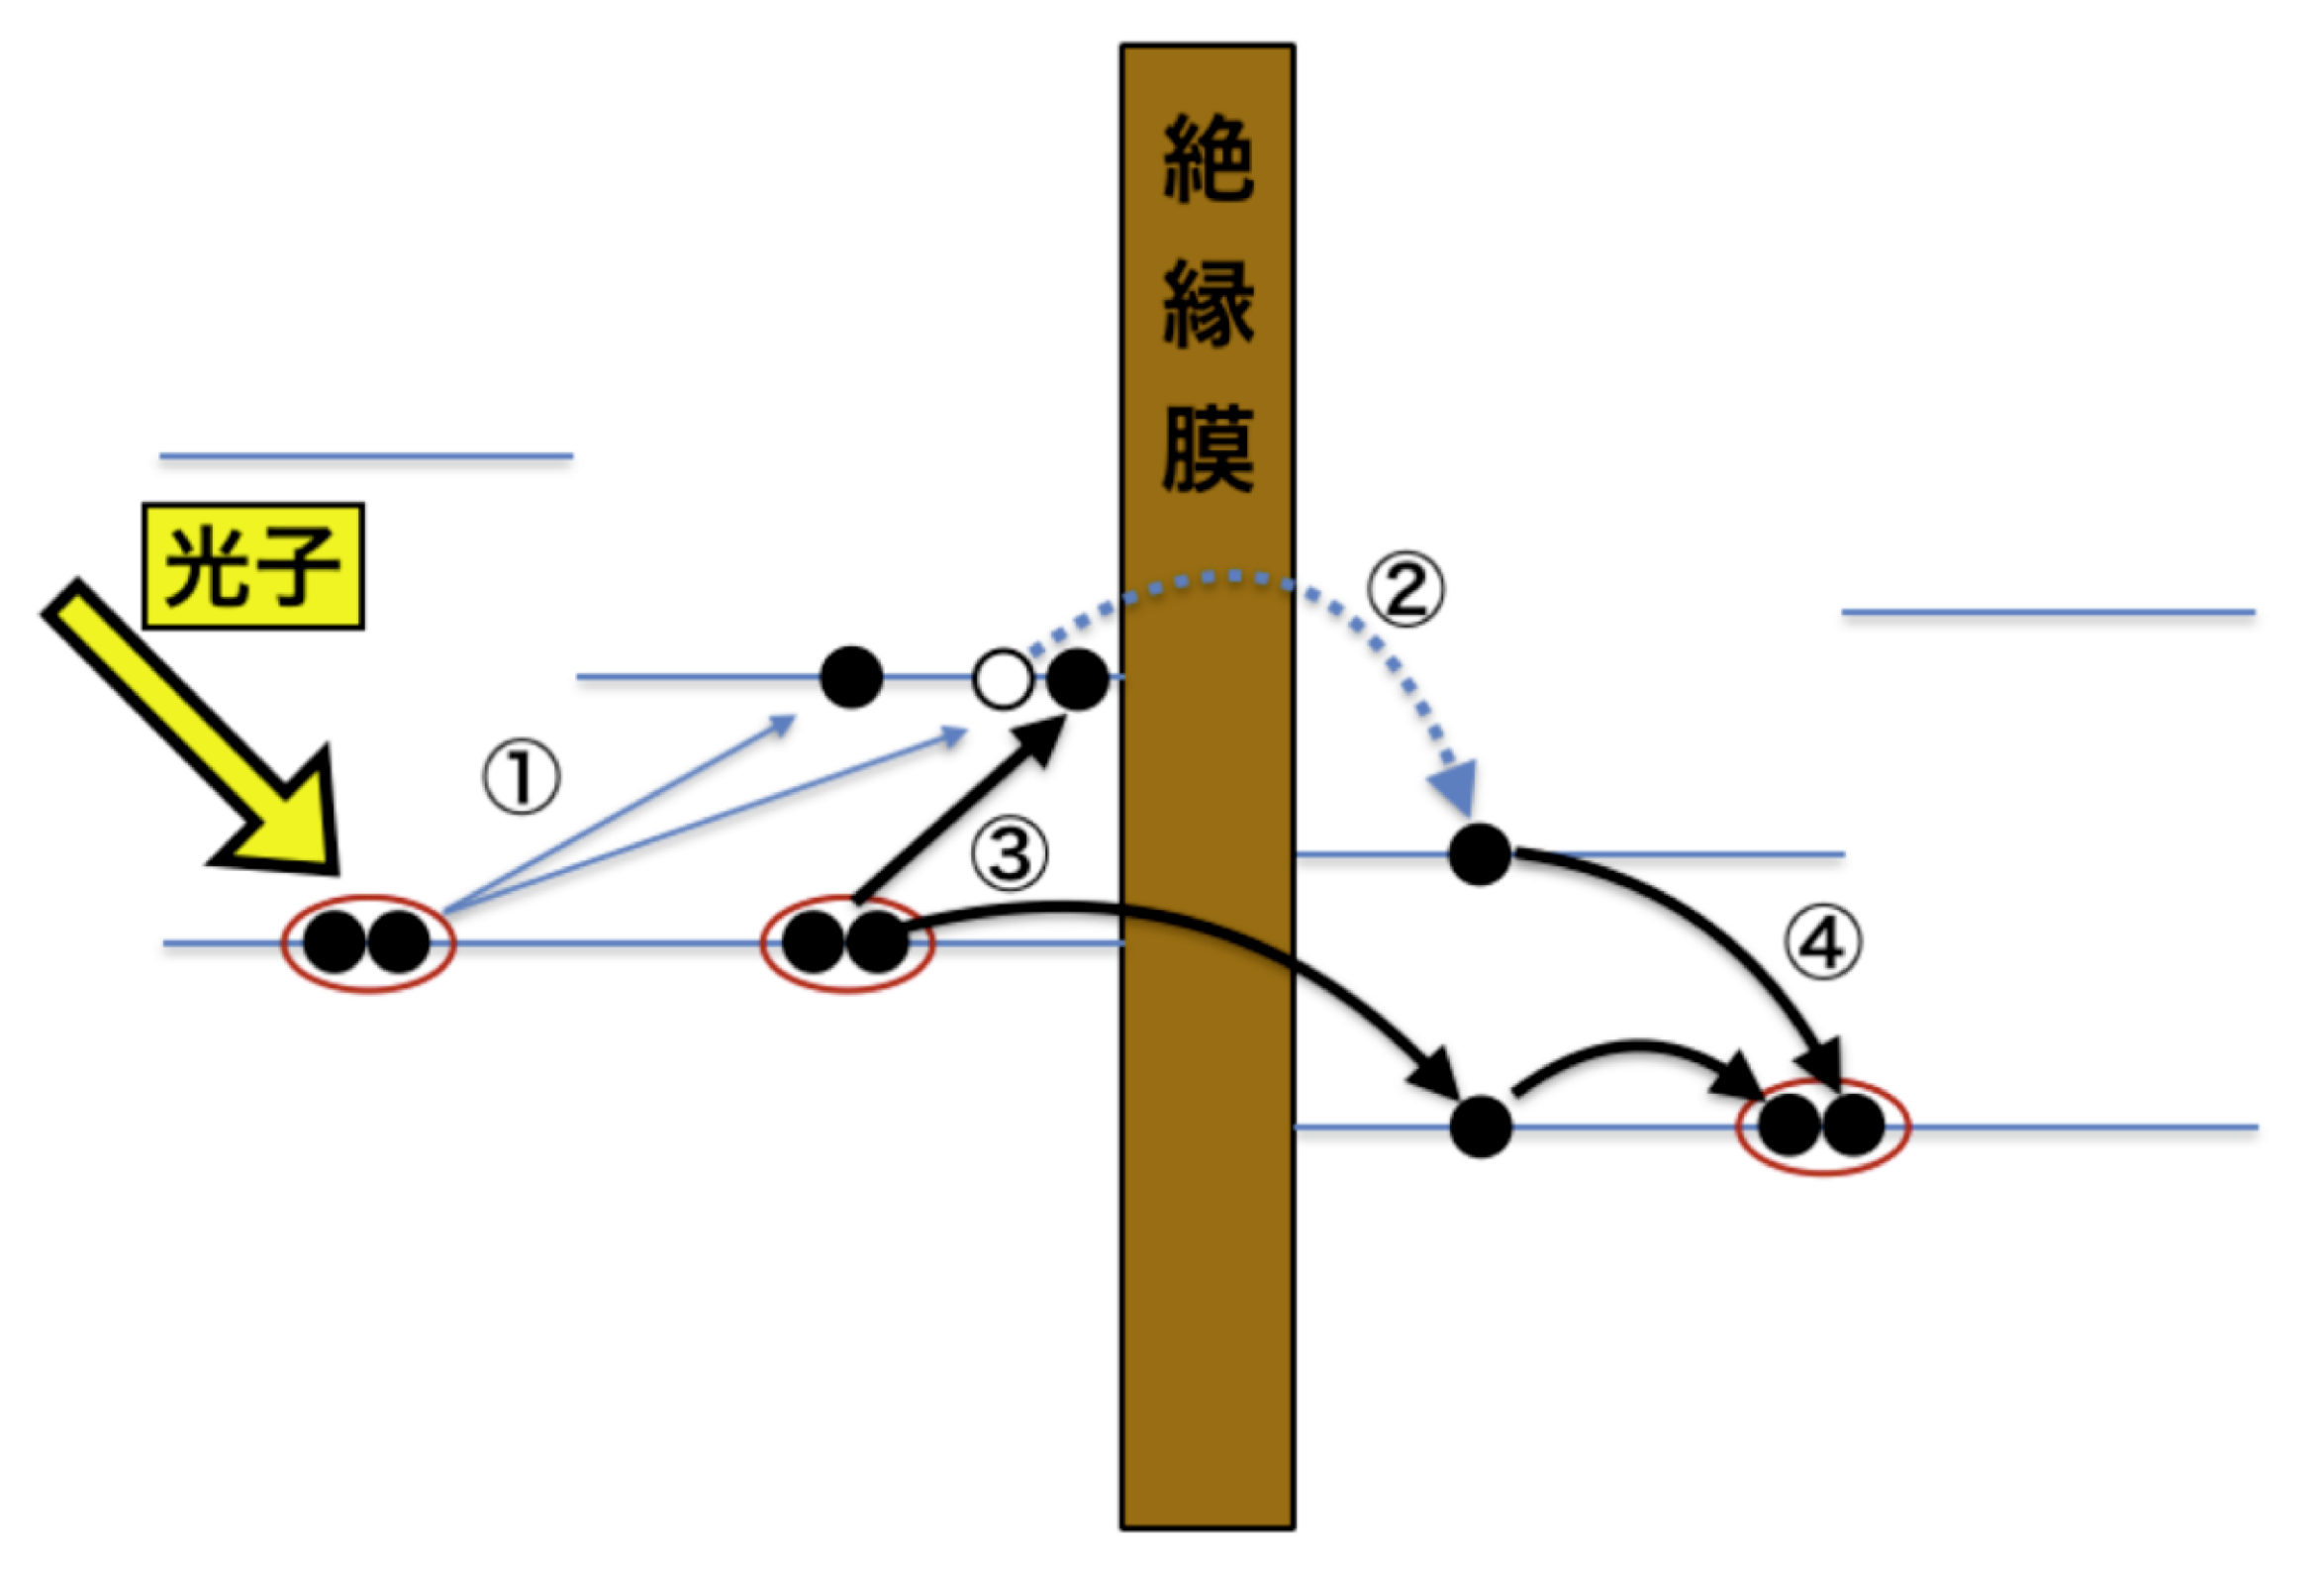
\includegraphics[width=12.0cm]{./Chapter/Chapter2/Picture/NbAlSTJ_backtunnel.eps}
    						\caption{バックトンネリング効果の概念図}
	  					\label{fig:NbAlSTJ_backtunnel}
  					\end{center}
				\end{figure}
				Nb/Al-STJ検出器のように、超伝導体と絶縁膜の間によりエネルギーギャップが小さい超伝導体を挟むことでトンネルする準粒子数が増加する、バックトンネリング効果が現れる。図\ref{fig:NbAlSTJ_backtunnel}にバックトンネリング効果の概念図を載せる。
				
				バックトンネリング効果の流れは以下のようになる。
				\begin{enumerate}
					\item STJ検出器の上部伝導体に入射した粒子がクーパー対を壊し、2つの準粒子を発生させる。
					\item 2つの準粒子のうち、1つは上部超伝導体のAl層の常伝導体にトラップされて、もう1つは絶縁膜をトンネルして下部聴伝導体のAl層の常伝導体にトラップされる。
					\item 下部超伝導体にクーパー対を作ろうと、上部伝導体の別のクーパー対が壊されて新たに2つの準粒子が生成される。
					\item 先に絶縁膜をトンネルした粒子どうしが再結合してクーパー対をなす。
					\item 残された準粒子は上部超伝導体のAl層常伝導体でトラップされる
				\end{enumerate}
				この一連の流れを繰り返すことでトンネル準粒子数が増加、つまりトンネル電流が増加する。
				バックトンネリング効果を踏まえ、STJ検出器にエネルギーEを持つ粒子が入射したときの準粒子生成個数$N$は、
				\begin{eqnarray}
					N = G_{\mathrm{Al}} \frac{E}{1.7 \Delta}
				\end{eqnarray}
				となる。この$G_{\mathrm{Al}}$をトラッピングゲインと呼び、バックトンネリング効果によるトンネル準粒子数の増加率を表す。トラッピングゲイン$G_{\mathrm{Al}}$は約10倍程度とされている。
		\end{description}

	\subsection{Nb/Al-STJ検出器の研究開発の現状}
		本研究グループは2014年度から、産業技術総合研究所(AIST)との共同研究を開始した。
		そして、Nb/Al-STJ検出器素子作製は産業技術総合研究所のCRAVITY(Clean Room for Analog-digital superconductiVITY)で行なわれている。
		ここでは安定して高品質の超伝導素子を作製することができる。
		
		図\ref{fig:NbAlSTJ_leaktemp}にCRAVITYで作製されたNb/Al-STJ検出器のリーク電流の温度依存性を示す。
		素子のサイズは$50 \times 50 \mathrm{{\mu m}^2}$である。
		この図からわかるように、0.4K程度以下でリーク電流が飽和することがわかる。この飽和したリーク電流は熱起因ではないリーク電流であり、より高品質のSTJ検出器素子作製や測定系の改善を行うことで下げることができる。
		25meVの一光子をリーク電流の揺らぎに対して$3 \sigma$以上で検出するためには、STJ検出器の信号幅を$1 \mathrm{\mu s}$と仮定すると、STJ検出器のリーク電流要求値は100pA以下である必要がある。
		表\ref{tab:NbAlSTJ_leaksize}に、我々が測定したNb/Al-STJ検出器のサイズごとのリーク電流値を示す。この表からCRAVITY製のNb/Al-STJ検出器はCOBAND実験のリーク電流の要求値を満たしていることがわかる。
		
		しかし、現在もなおNb/Al-STJ検出器を用いて遠赤外光一光子検出の成功には至っていない。その理由として、STJ検出器からの信号を冷凍機外部へと長い配線を経て読み出す際に、測定系由来の雑音がSTJ検出器信号に大きく効いてきてしまうからだ。この問題の解決策として、STJ検出器が動作する極低温環境下においても動作可能な前置増幅器を冷凍機内に設置し、STJ検出器信号が雑音に埋もれてしまう前に増幅する方法がある。\\
		我々は現在、この極低温前置増幅器の研究開発を行なっており、次章はこれについて詳しく述べる。
		%=====Nb/Al-STJのリーク電流温度依存性のplotを載せる=====%
		\begin{figure}[htbp]
  			\begin{center}
  				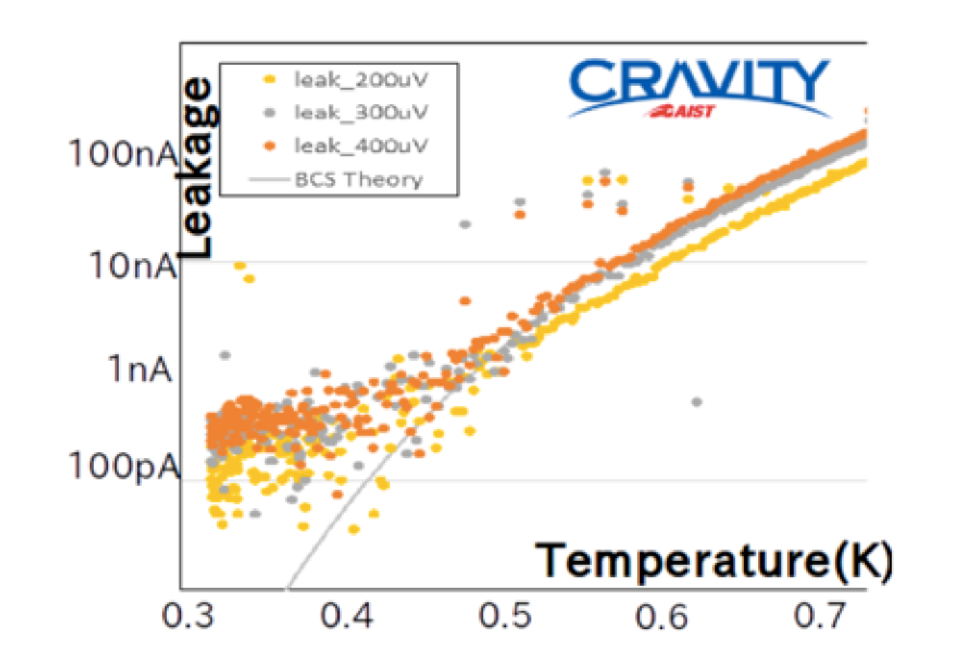
\includegraphics[width=8.0cm]{./Chapter/Chapter2/Picture/NbAlSTJ_leaktemp.eps}
    				\caption{CRAVITY製Nb/Al-STJ検出器のリーク電流温度依存性}
	  			\label{fig:NbAlSTJ_leaktemp}
 			\end{center}
		\end{figure}
		%=====現在のリーク電流の状況を表にして載せる=====%
		\begin{table}[htb]
			\begin{center}
				\caption{CRAVITY製Nb/Al-STJ検出器のサイズごとのリーク電流値}
				\begin{tabular}{| l || c | c | c |} \hline
					Nb/Al-STJのサイズ & ${100 \mathrm{\mu m}}^2$ & ${50 \mathrm{\mu m}}^2$ & ${20 \mathrm{\mu m}}^2$ \\ \hline
					リーク電流$I_{\mathrm{leak}}$@0.4mV & 2 nA & 300 pA & 100 pA \\ \hline
				\end{tabular}
				\label{tab:NbAlSTJ_leaksize}
			\end{center}
		\end{table}
	 %超電導トンネル接合素子光検出器(STJ)
	%\chapter{SOIピクセル検出器}

\section{概要}

2005年4月よりKEK測定器開発室のプロジェクトの一つとしてSilicon On Insulator(以下SOI)技術による読み出し回路一体型ピクセル検出器の開発が開始された.SOI技術とは、回路部シリコン層と支持基板部シリコン層間に${\rm SiO_2}$の絶縁層を埋め込む技術であり、トランジスタ素子を分離することで電気的な接続を分離できるのが特徴である.読み出し回路部から検出部分へは酸化膜層BOX(Buried OXide)を貫通する金属ビアを通したセンサー電極が伸びており、センサー電極シリコンと検出部分シリコンのpn接合で検出部分に空乏層を形成する.そこに逆バイアス電圧を印加することで空乏層を広げる.空乏層へ荷電粒子が入射すれば、電子正孔対が生成され、センサー電極に移動しシグナルとして検出される.よって、どこのセンサー電極で検出されたかによって入射粒子の通過した位置を決めることができる。このSOI技術を用いることで、現在主流であるバルクCMOS技術と同じ設計ルールでも一世代進んだ特性を示す半導体を製造することが可能であり、KEKの新井康夫氏を中心にR$\&$Dが進められてきた.特に、2013年から本年度に掛けて、「3次元半導体検出器で切り拓く新たな量子イメージングの展開」として新学術領域研究に指定され、素核・宇宙・物質・生命科学の多岐に渡りSOI技術を用いた新たな量子イメージング領域の研究が行われてきた.

\begin{figure}[htbp]
			\begin{center}
				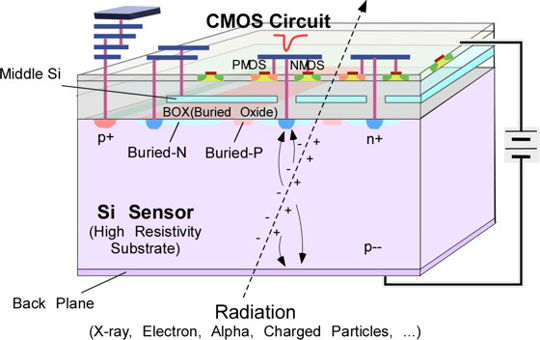
\includegraphics[width=12.0cm]{./Chapter/Chapter3/Picture/SOIPIX.png}
				\caption{SOIピクセル検出器}
				\label{fig:SOIPIX}
			\end{center}
		\end{figure}
%\begin{figure}[H]
%\begin{center}
%\includegraphics[width=120mm]{./Chapter/Chapter3/Picture/SOIピクセル検出器.png}
%\end{center}
%\caption{SOIピクセル検出器}
%\label{fig:SOI}
%\end{figure}
%\end{section}
%\clearpage

\section{SOIウエハーの特徴}
SOI技術を用いることの利点を具体的に説明する.

\section{Monolithic型検出器}
現在多くの放射線イメージセンサーには



身近にある物質の中でも金属のように電気を通すものもあれば、ガラスのように電気をほとんど通さないような物質も存在する。抵抗率の違いから、物質は大きく3種類に大別されている。
	\begin{description}
		\item[導体] 金属など電気を通しやすい物質
		\item[絶縁体] ガラスのように電気を通しにくい物質
		\item[半導体] 導体と絶縁体の中間の抵抗率を持つ物質
	\end{description}
	
	この半導体には「P型半導体」と「N型半導体」の2種類の型があり、以下それらについて説明する。
	\subsection{P型半導体とN型半導体}
		シリコンは価電子を4個持つ。純粋なシリコンの結晶中では隣り合ったシリコン原子は互いに電子を共有しあって結合している。電子は原子に束縛されている状態なので容易に動くことはできない。したがって純粋なシリコン結晶に電圧を印加しても電流はほとんど流れず、電気抵抗率は室温環境下で$10^3 \mathrm{\Omega cm}$以下である。
		
		しかし、シリコンに不純物を添加した状態で電圧を印加することによってキャリアを流すことができる。添加する物質の違いから、
		\begin{description}
			\item[P型半導体] キャリアが正孔である半導体
			\item[N型半導体] キャリアが電子である半導体
		\end{description}
		に大別することができる。P型半導体とN型半導体の概念図を図\ref{fig:Semicon_PN}に示す。
		
		P型半導体は高純度の半導体(主にシリコン)に不純物としてホウ素Bなどの3価元素をごく微量添加することによって作製できる。
		シリコンSiの価電子が4個に対して、ホウ素Bのような3価元素の価電子は3個しかないので、共有結合するのに電子が1つ足りない状況になる。
		したがって、図\ref{fig:Semicon_P}のように電子のない空席(これを「正孔」と呼ぶ)ができる。
		不純物を添加しない場合、電子は原子に束縛された状況なので動くことはできないが、ホウ素Bを添加することで正孔ができるので、結晶に電圧を印加した場合、正孔の近くにある電子は正極に引かれて正孔の方に移動する。
		そのとき、その電子がもともと存在していた場所は新たな正孔となり、その近くに存在する電子がまた移動し、正孔があたかも正(positive)の電荷を持つ粒子のように振る舞う。
		このような半導体のことを「P型半導体」と呼び、この半導体のキャリアは正(positive)の電荷を持つ「正孔」である。
		
		一方、N型半導体は高純度シリコンSiに不純物としてリンPなどの5価元素をごく微量添加することによって作製できる。
		5価元素の価電子は5個なので共有結合に電子を4個使っても電子が1つ余ってしまう。
		共有結合に使われている他の電子に比べてリン原子との束縛は弱いので、結晶に電圧を印加することによって電子は正極に引かれて動く。
		このような振る舞いを示す半導体のことを「N型半導体」と呼び、この半導体のキャリアは負(negative)の電荷を持つ「電子」である。
		%=====P型半導体とN型半導体の概念図を載せる=====%
		\begin{figure}[hbtp]
  			\begin{minipage}[b]{0.45\linewidth}
    				\centering
    				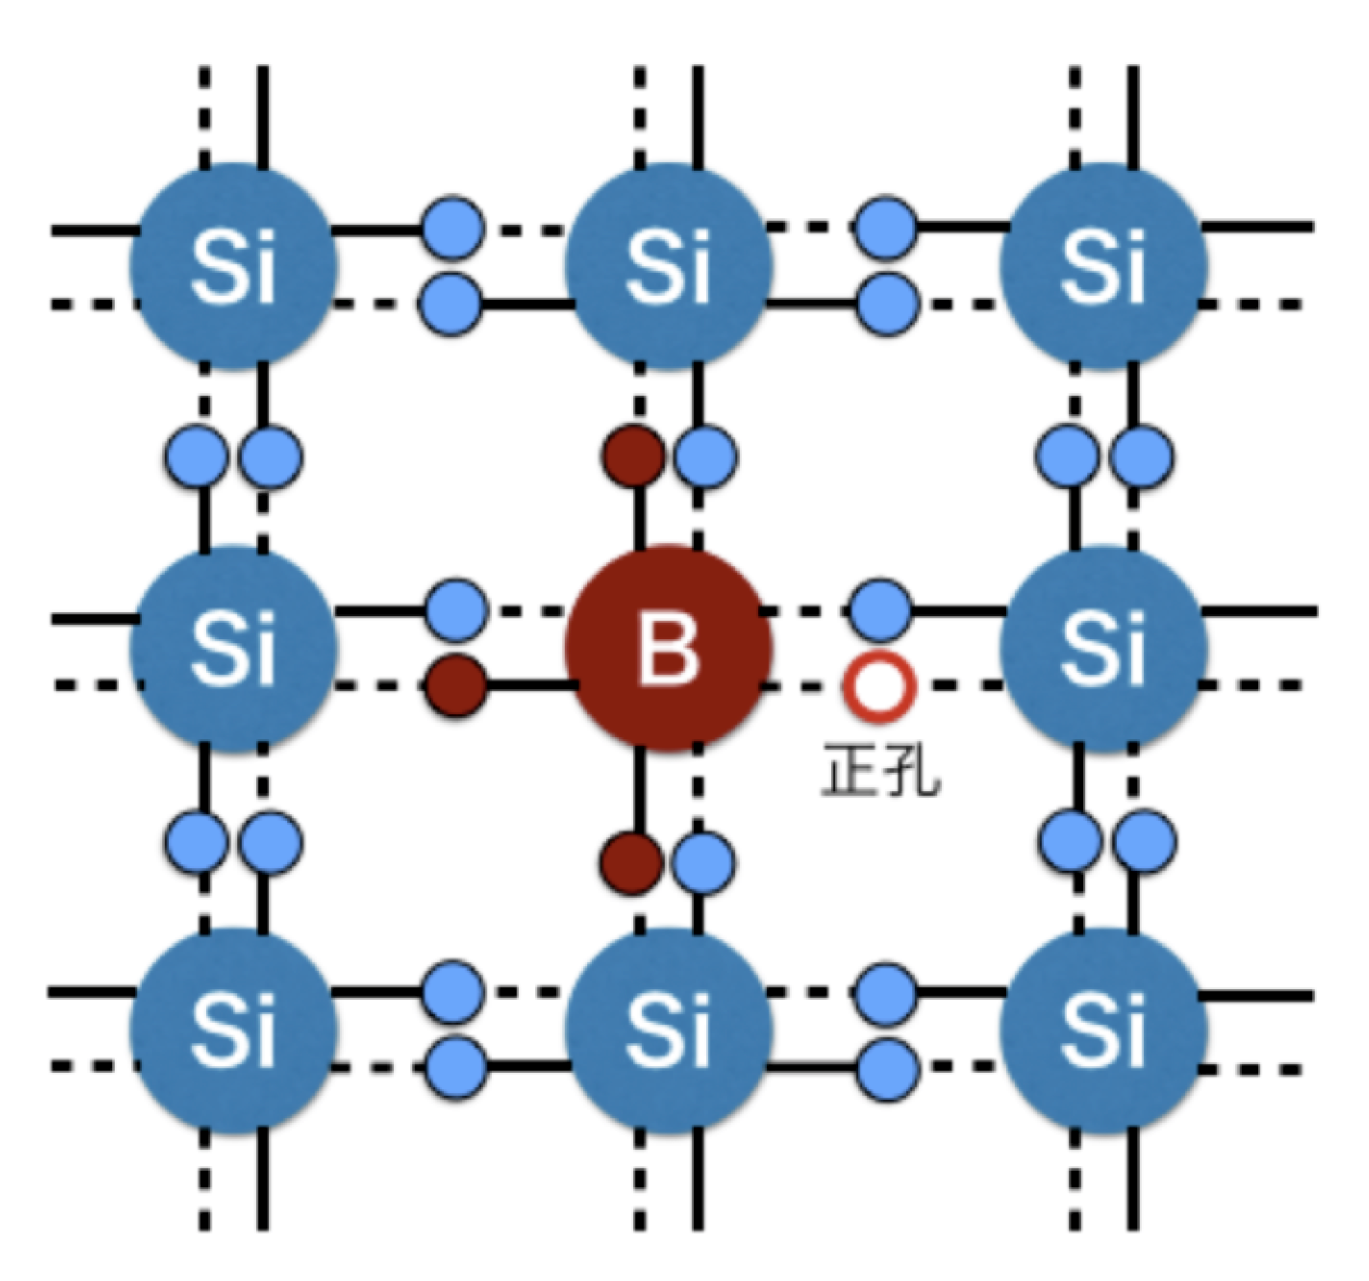
\includegraphics[keepaspectratio, scale=0.2]{./Chapter/Chapter3/Picture/Semicon_P.eps}
				\subcaption{P型半導体}
				\label{fig:Semicon_P}
  			\end{minipage}
  			\begin{minipage}[b]{0.45\linewidth}
    				\centering
    				\includegraphics[keepaspectratio, scale=0.2]{./Chapter/Chapter3/Picture/Semicon_N.eps}
    				\subcaption{N型半導体}
				\label{fig:Semicon_N}
  			\end{minipage}
 			\caption{P型半導体とN型半導体のそれぞれの概念図}
			\label{fig:Semicon_PN}
		\end{figure}
		
		半導体を用いたデバイスには2端子を基本とする「ダイオード」と3端子を基本とする「トランジスタ」がある。
		そのトランジスタには動作原理から、「電界効果トランジスタ(FET : Field Effect Transistor)」と「バイポーラトランジスタ(BJT : Bipolar Junction Semiconductor)」に大別される。
		
		我々研究グループが開発している極低温環境用前置増幅器には、この2種類のトランジスタのうちMOS(Metal Oxide Semiconductor)構造を持った電界効果トランジスタ(MOSFET)を用いることを考えている。次節は、そのMOSFETについての基礎特性について述べる。
		
\section{MOSFETの基礎}
	MOSFETには3つの端子があり、それぞれソース(S)、ゲート(G)、ドレイン(D)とよばれている。ゲート・ソース間に電圧を印加することによって、ドレイン・ソース間のキャリア密度が変化し、それによってドレイン・ソース間の電流(ドレイン電流)を制御することができる。MOSFETはドレイン・ソース間を移動するキャリアの種類によって2つの型に大別することができる。キャリアが電子の場合はN型MOSFET(NMOS)と呼ばれ、正孔の場合はP型MOSFET(PMOS)と呼ばれる。
	\subsection{MOSFETの構造}
		前述した通り、MOSFETはキャリアの種類に応じてNMOSとPMOSの2種類に大別される。図\ref{fig:MOSFET_N_structure}にNMOSの構造を示した。
		以降、NMOSについての構造について述べる。
	%=====MOSFETの構造の概念図を載せる=====%
		\begin{figure}[htbp]
			\begin{center}
				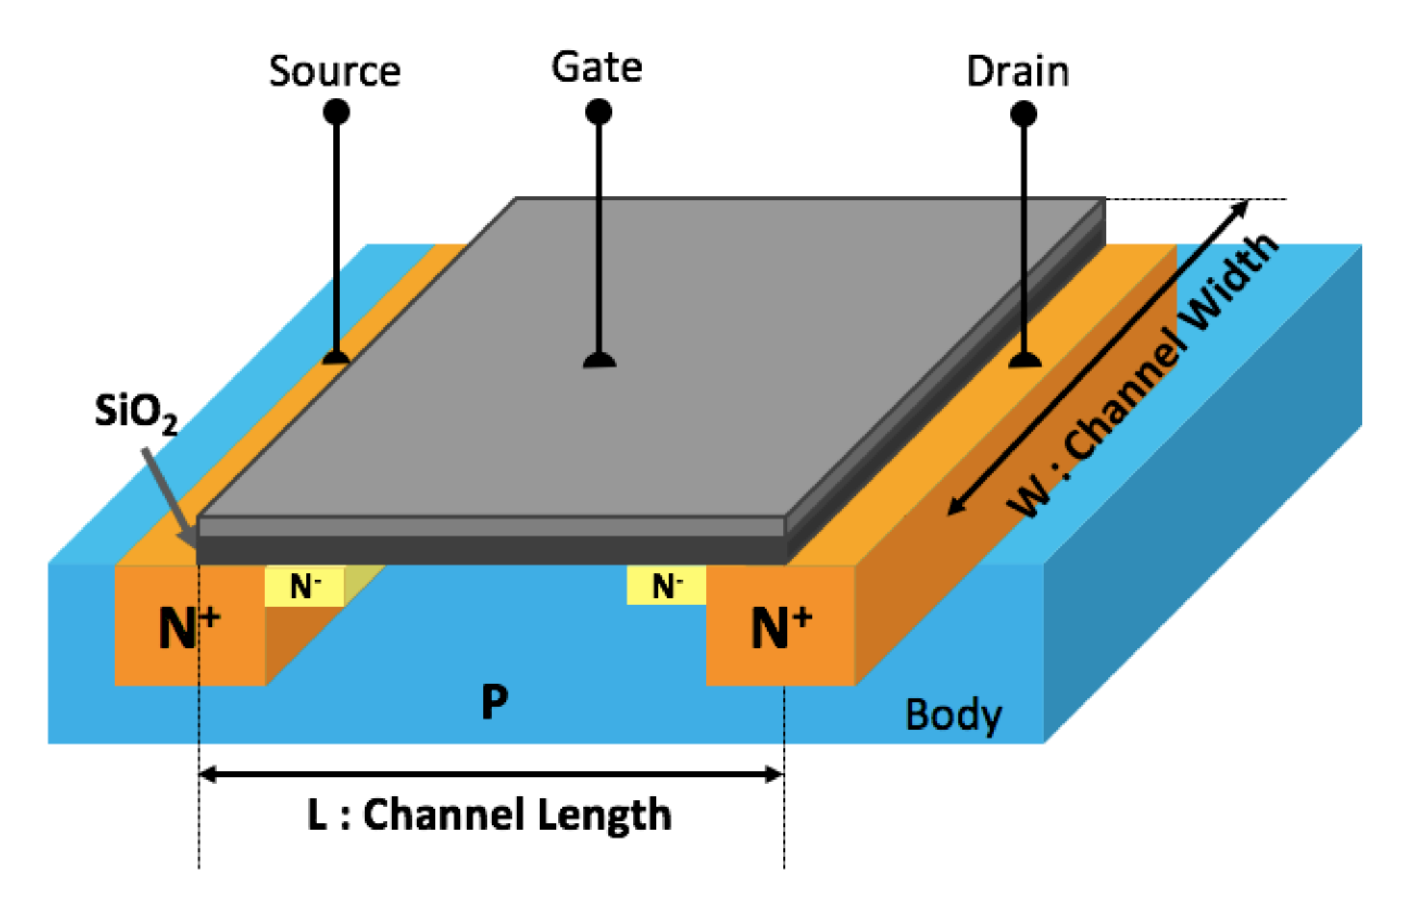
\includegraphics[width=12.0cm]{./Chapter/Chapter3/Picture/MOSFET_N_structure.eps}
				\caption{N型MOSFETの構造}
				\label{fig:MOSFET_N_structure}
			\end{center}
		\end{figure}
		P型半導体基板上に$\mathrm{N^+}$領域が2つ形成されており、それぞれソース(S : Source)、ドレイン(D : Drain)と呼ばれている。
		そして、これらの$\mathrm{N^+}$領域に挟まれたP型半導体基板の直上に酸化シリコン$\mathrm{SiO_2}$からなるゲート酸化膜が形成されており、そして更に直上に金属、あるいはポリシリコンからなるゲート電極(G : Gate)が形成されている。
		また、PN接合近傍での急激な電界勾配を回避するために、ゲートエッジ部にソースとドレインそれぞれの拡散層の不純物密度分布を緩やかにするプロセスが施されている。
		この部分を低濃度不純物ドレイン(LDD : Lightly Doped Drain)と呼ぶ。
		一方、PMOSの構造は、NMOSで用いる半導体の型を反転した構造をしており、それ以外の構造はNMOSと同じである。次節ではMOSFETの動作原理について述べる。
	\subsection{MOSFETの動作原理}
		\begin{figure}[htbp]
			\begin{center}
				\begin{tabular}{c}
					\begin{minipage}{0.33\hsize}
						\begin{center}
							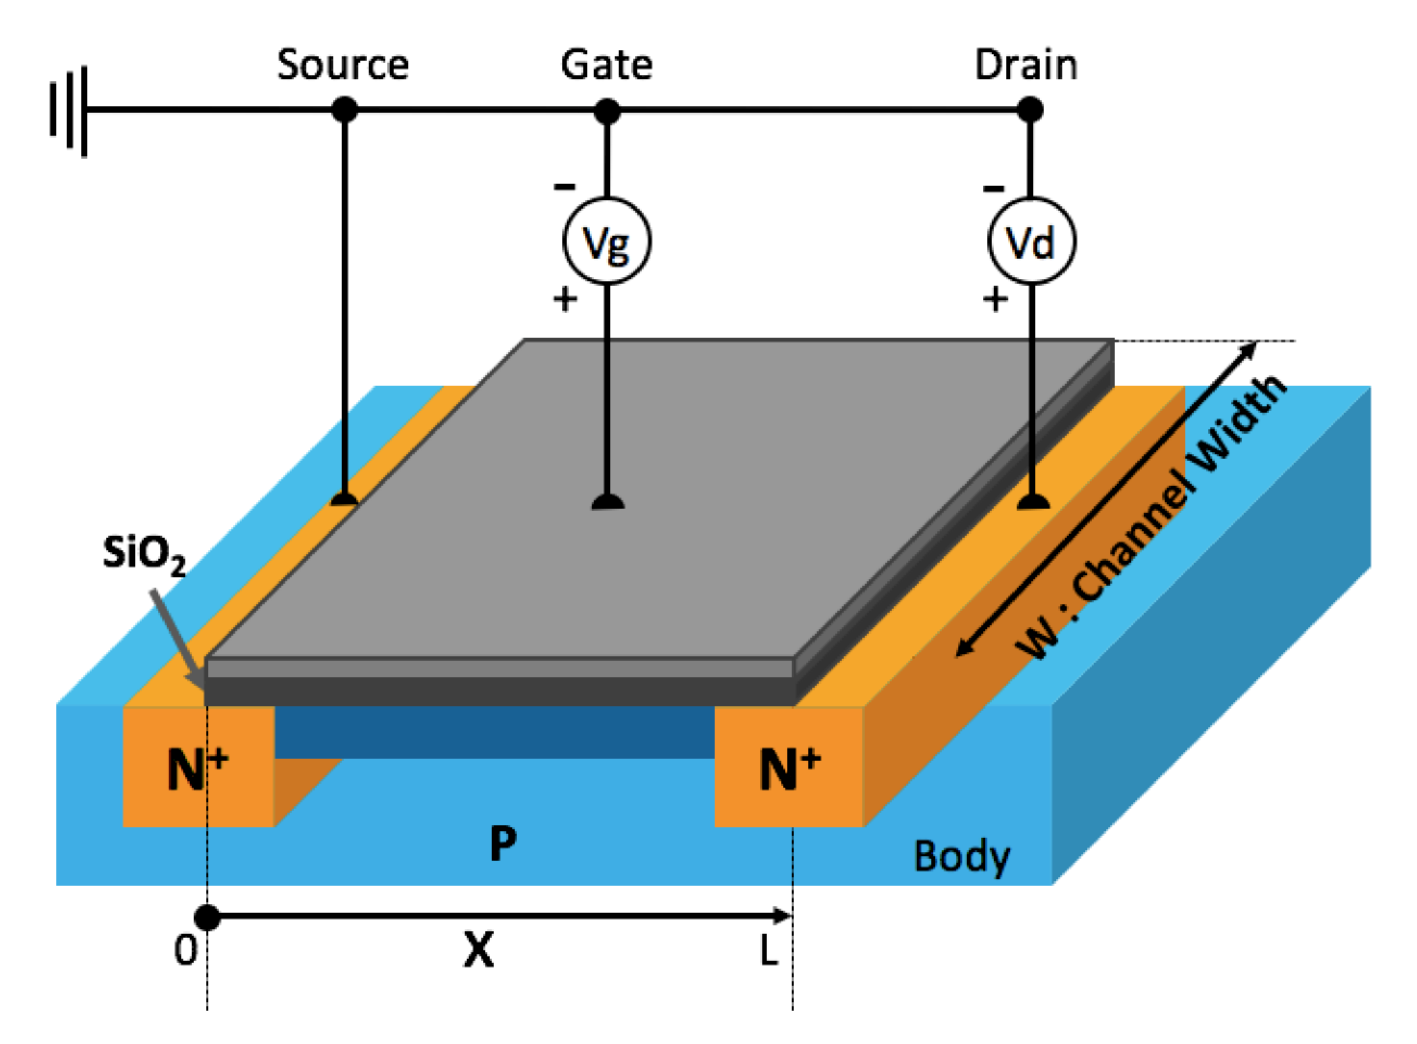
\includegraphics[clip, width=4.5cm]{./Chapter/Chapter3/Picture/MOSFET_accumulation.eps}
							\hspace{1.6cm} [1]蓄積領域
						\end{center}
					\end{minipage}
					\begin{minipage}{0.33\hsize}
						\begin{center}
							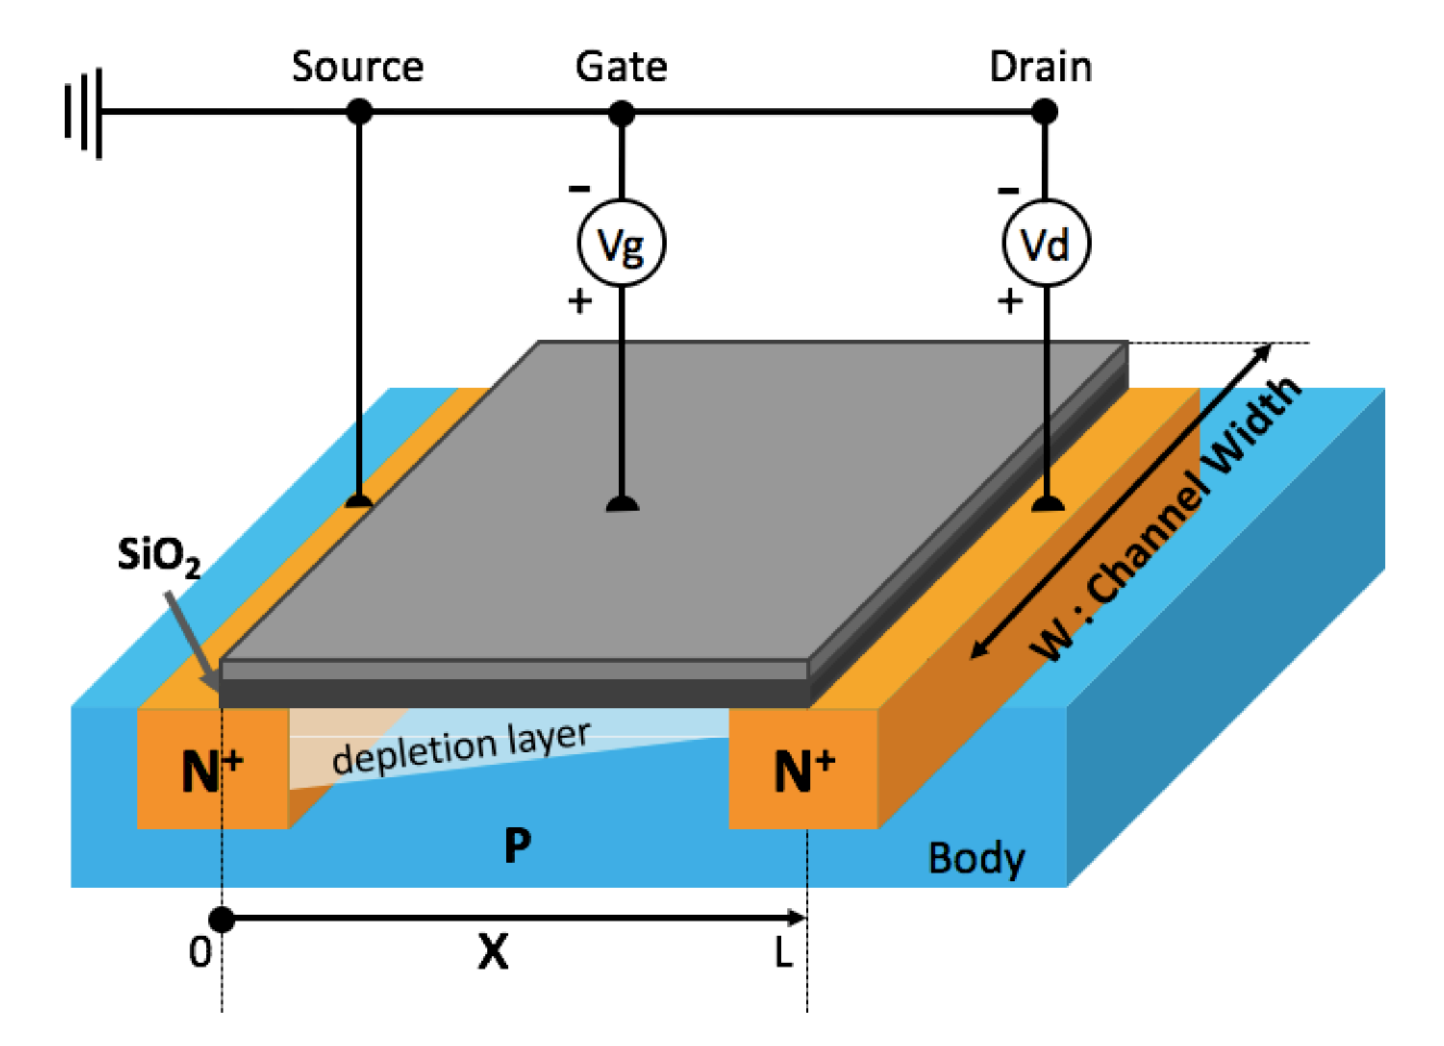
\includegraphics[clip, width=4.5cm]{./Chapter/Chapter3/Picture/MOSFET_depletion.eps}
							\hspace{1.6cm} [2]空乏領域
						\end{center}
					\end{minipage}
					\begin{minipage}{0.33\hsize}
						\begin{center}
							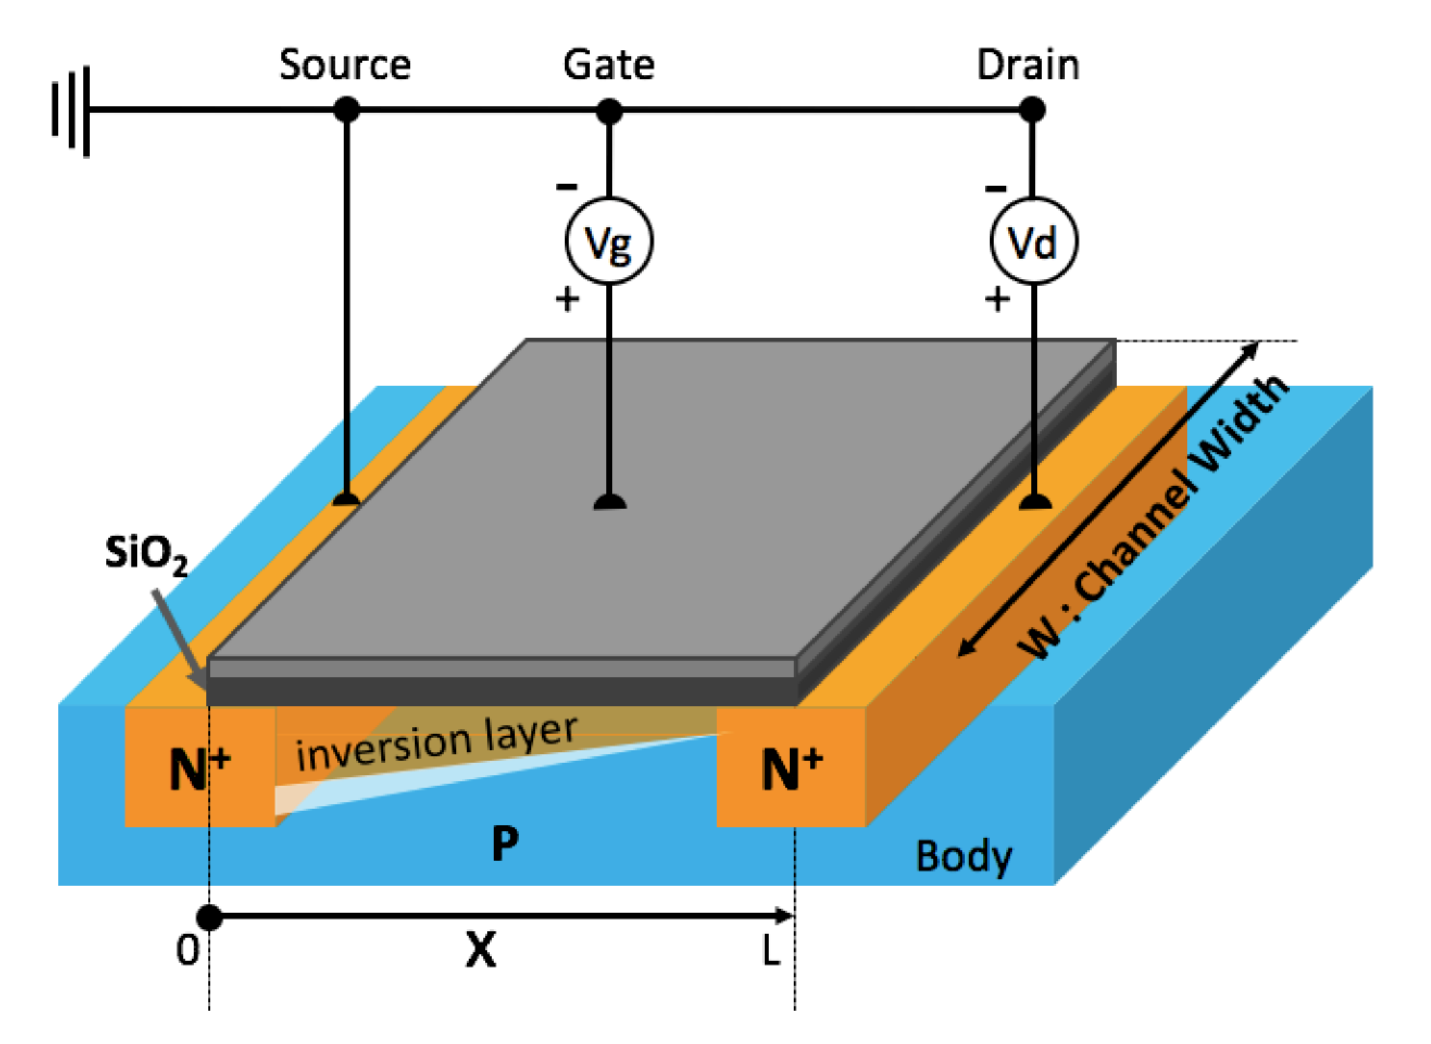
\includegraphics[clip, width=4.5cm]{./Chapter/Chapter3/Picture/MOSFET_inversion.eps}
							\hspace{1.6cm} [3]反転領域
						\end{center}
					\end{minipage}
				\end{tabular}
				\caption{NMOS動作原理概念図}
				\label{fig:MOSFET_N_WorkingPrinciple}
			\end{center}
		\end{figure}
		図\ref{fig:MOSFET_N_WorkingPrinciple}にNMOSの場合の動作原理概念図を示した。
		MOSFETの各端子に電圧を印加した際、MOSFETがどのような振る舞いを示すかを述べる。
		
		ゲート電圧が負の場合、ゲート直下には正孔が誘起される。
		このときの振る舞いは図\ref{fig:MOSFET_N_WorkingPrinciple}[1]のようになり、蓄積領域と呼ばれる。
		このときドレインとソースは強く分離され電流は流れない。
		そして、ゲート電圧が正の場合、ゲート直下には電子が誘起され、誘起された電子はP型基板中の正孔と結合して空乏層が形成される。
		このときの振る舞いは図\ref{fig:MOSFET_N_WorkingPrinciple}[2]のようになり、空乏領域と呼ばれる。
		この領域でもドレイン・ソース間に電流は流れない。
		さらに、ゲート電圧を上昇させると、ゲート直下に誘起される電子密度がP型基板の正孔密度を上回り、その結果ゲート直下の半導体の型がP型からN型へ反転した状態になる。
		この層のことを反転層と呼ぶ。
		このときの振る舞いは図\ref{fig:MOSFET_N_WorkingPrinciple}[3]のようになり、反転領域と呼ばれる。
		このときソースとドレインは反転したN型半導体で繋がれた状態になり、ドレインからソースへ電子の移動が可能になる。このときの電子(キャリア)の通り道のことをチャネルと呼ぶ。
		この結果ソースからドレインへ電流が流れるようになり、このときにMOSFETはONになる。
		そして更にゲート電圧を上昇させると、反転層が厚くなるのでより電流が流れるようになる。
		
		しかし、ゲート電圧を上げ過ぎると、ゲート酸化膜が壊れてしまう危険性がある。このゲート酸化膜は静電気でも壊れてしまう。
		したがって、電圧を印加する際や保管の際は十分注意が必要である。
		MOSFETの保管の際は静電気による絶縁破壊を防ぐために各端子をショートさせて保管する。
		そして実際にMOSFETを動作させるときは静電気バンド等を用いてしっかり静電気対策を行う必要がある。
		本節ではMOSFETのドレイン電流と各端子に印加する電圧依存性について詳しく述べる。
	\subsection{MOSFETの電流電圧特性}
		%=====IdVd plot(NMOS)を載せる=====%
		\begin{figure}[htbp]
			\begin{center}
				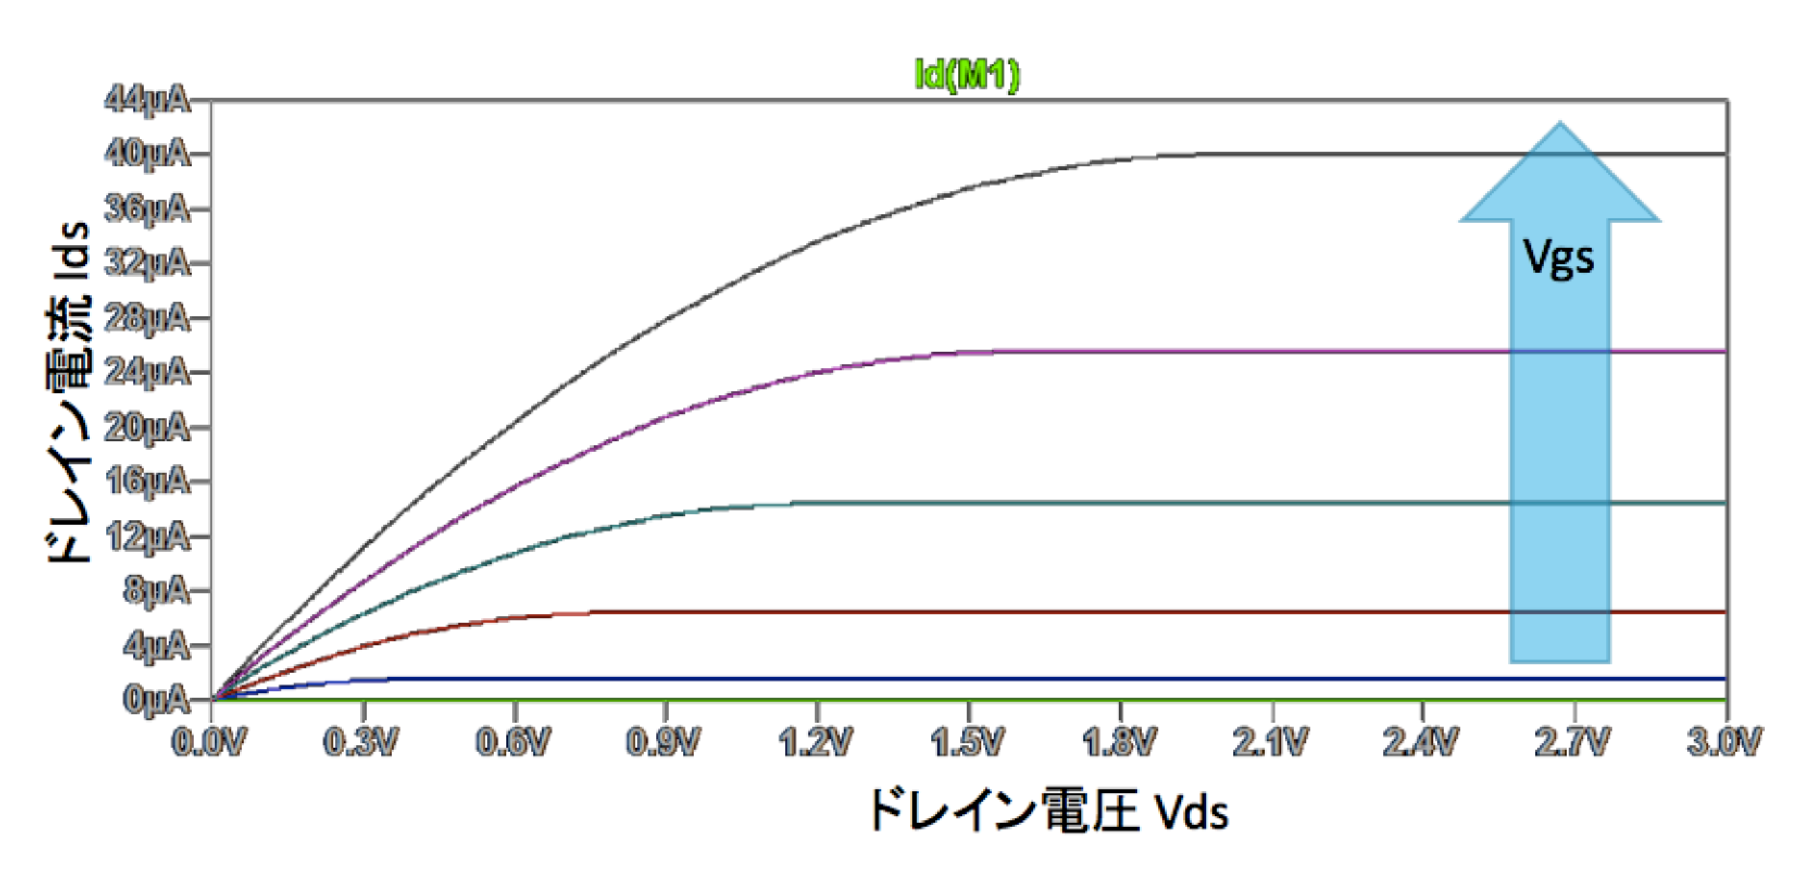
\includegraphics[width=12.0cm]{./Chapter/Chapter3/Picture/MOSFET_N_IdVd.eps}
				\caption{N型MOSFETのドレイン電流のドレイン電圧依存性}
				\label{fig:MOSFET_N_IdVd}
			\end{center}
		\end{figure}
		%=====IdVg plot(NMOS)を載せる (左 : log scale   右 : linear scale)=====%
		\begin{figure}[htbp]
			\begin{minipage}{0.5\hsize}
				\begin{center}
					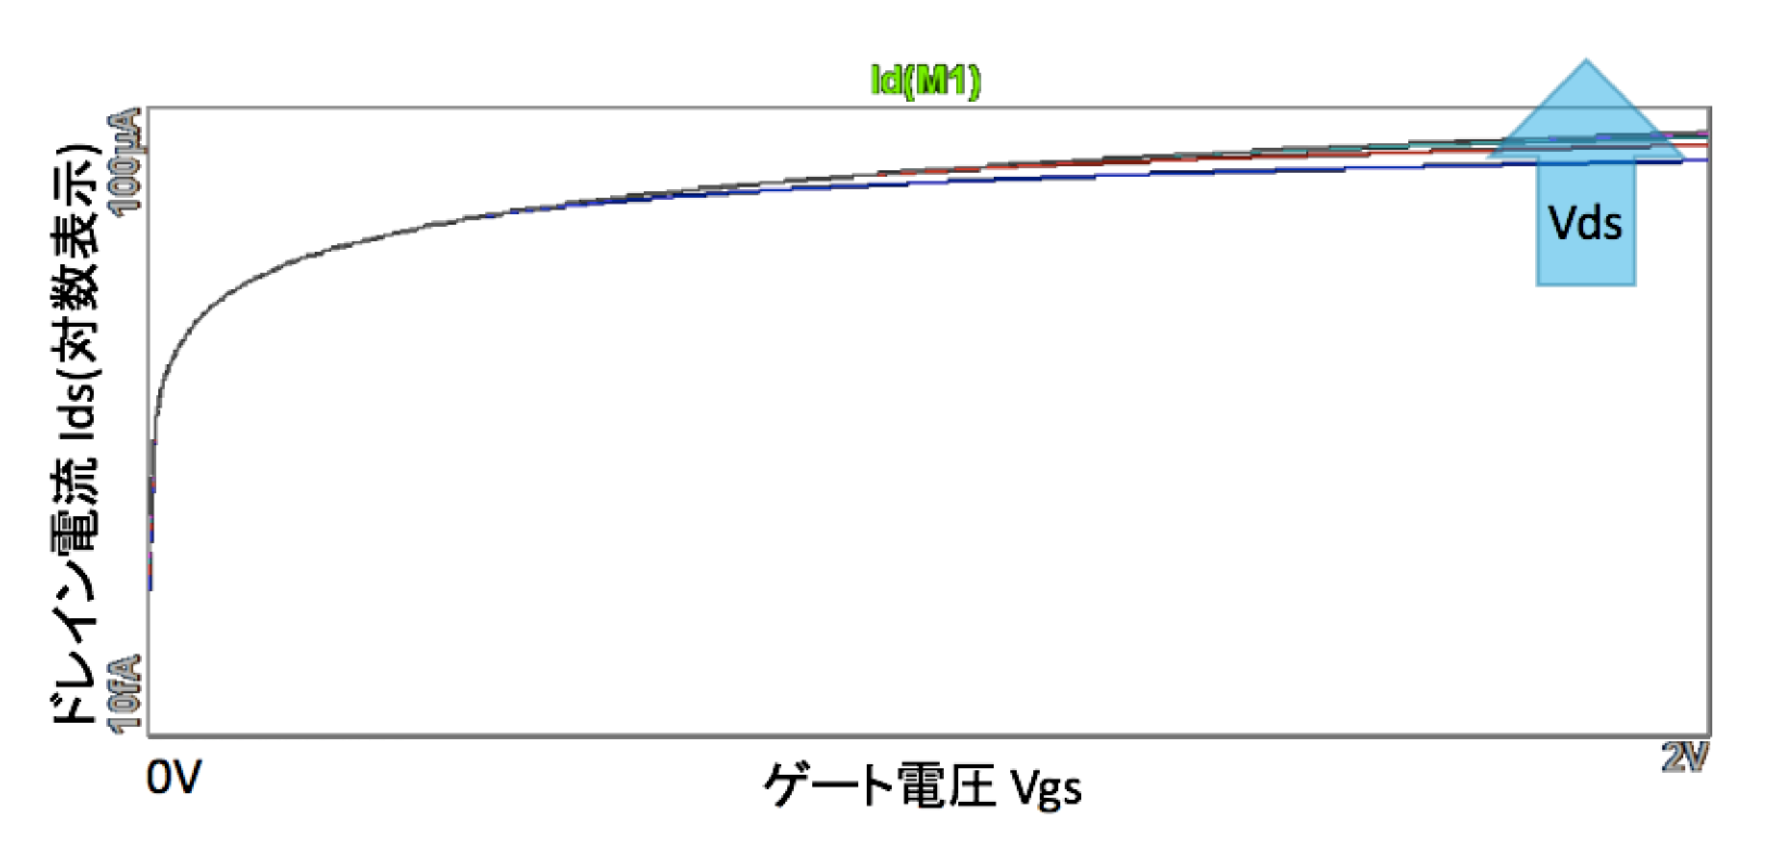
\includegraphics[width=70mm]{./Chapter/Chapter3/Picture/MOSFET_N_IdVg_log.eps}
				\end{center}
				\caption{N型MOSFETのドレイン電流のゲート電圧依存性(縦軸:対数表示)}
				\label{fig:MOSFET_N_IdVg_log}
			\end{minipage}
			\begin{minipage}{0.5\hsize}
				\begin{center}
					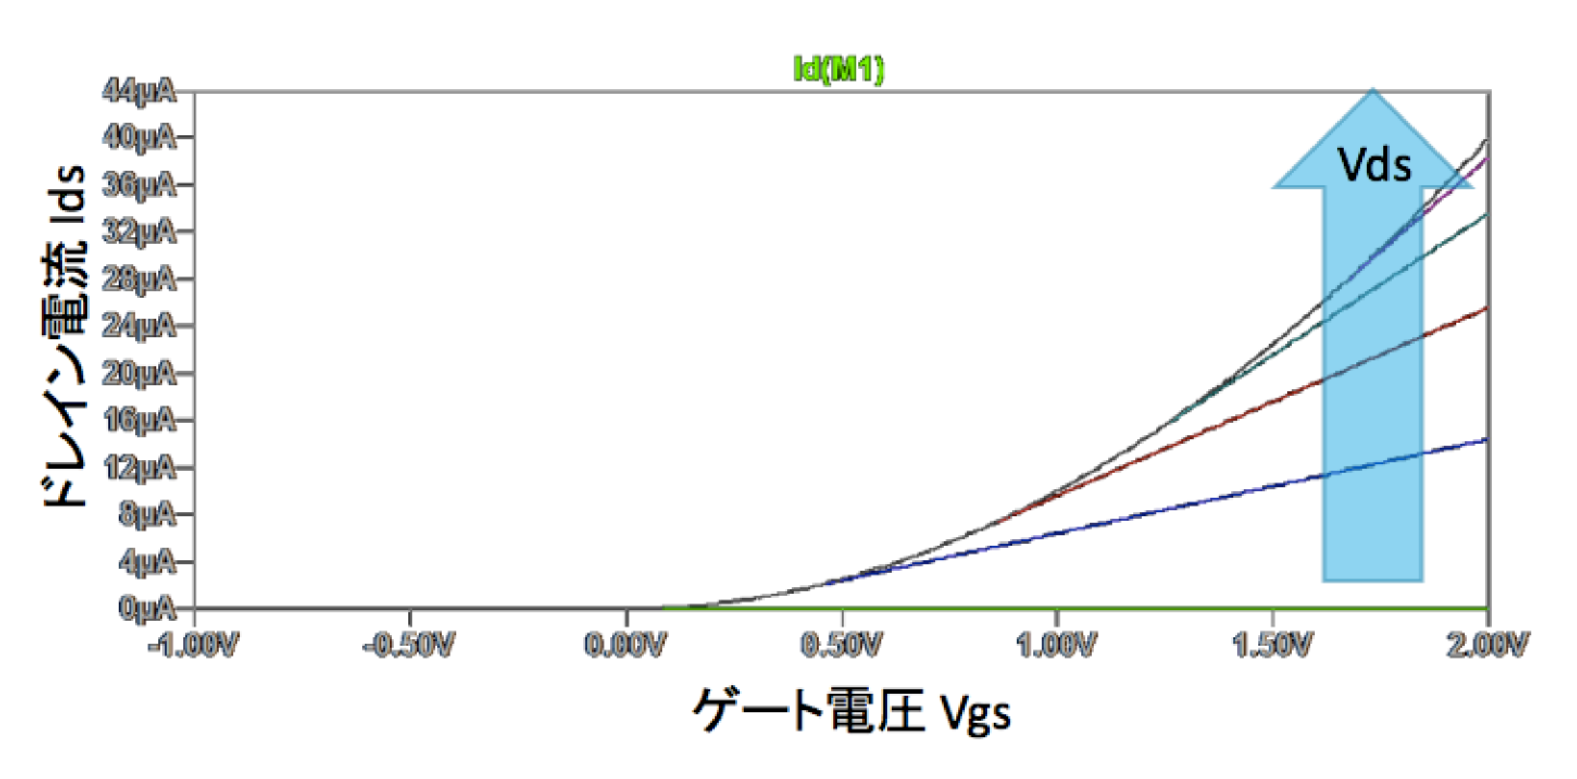
\includegraphics[width=70mm]{./Chapter/Chapter3/Picture/MOSFET_N_IdVg_linear.eps}
				\end{center}
				\caption{N型MOSFETのドレイン電流のゲート電圧依存性(縦軸:線形表示)}
				\label{fig:MOSFET_N_IdVg_linear}
			\end{minipage}
		\end{figure}
		MOSFETの電流電圧特性について、まずドレイン電流の式について述べる。ここでも前節と同様にNMOSについての場合について考える。位置$x$におけるチャネルの電子密度は閾電圧$V_{th}$以上のゲート電圧$V_{gs}$に比例しており、式(\ref{eq:MOSFET_Q})のように書ける。
		\begin{eqnarray}
			Q(x) = W C_{OX}[V_{gs} - V_{th} - V(x)]
			\label{eq:MOSFET_Q}
		\end{eqnarray}
		$W$は図\ref{fig:MOSFET_N_structure}に示したチャネル幅、$C_{OX}$は単位長さ当たりのゲート端子の電気容量、$V(x)$は位置$x$でのチャネル電位のことを指す。
		ここで電子の移動度を$\mu_{e}$とすると、ドレイン電流$I_d$は電子速度$v = \mu_{e}E$の電荷$Q(x)$の流れを表す。
		ソース・ドレイン間、つまりチャネル間の電位$E$は、
		\begin{eqnarray}
			E = \frac{dV(x)}{dx}
		\end{eqnarray}
		と表される。したがって、以上からドレイン電流$I_d$は式(\ref{eq:MOSFET_Id})のように表される。
		\begin{eqnarray}
			I_d = - \mu_e Q(x) E = - \mu_e W C_{OX}[V_{ds} - V_{th} - V(x)] \frac{dV(x)}{dx}
			\label{eq:MOSFET_Id}
		\end{eqnarray}
		以下、ゲート電圧、ドレイン電圧の関係性から2つの領域に分けて、ドレイン電流の表式について詳しく述べる。
		\subsubsection{線形領域}
			ドレイン電圧とゲート電圧の関係性が、$V_{ds} < V_{gs} - V_{th}$のときを「線形領域」と呼ぶ。
			このときチャネルはドレイン・ソース間にまたがっており、$V(L)=V_{ds}$である。
			境界条件として、$V(x=0) = 0$、$V(x=L)=V_{ds}$とする。
			式(\ref{eq:MOSFET_Id})の両辺に$dx$をかけて、積分する。
			\begin{eqnarray}
				\int_{x=0}^{x=L} I_{ds} dx = \int_{V=0}^{V=V_{ds}} W C_{OX} \mu_e [V_{ds} - V_{th} - V(x)] dV
				\label{eq:MOSFET_Id_linear1}
			\end{eqnarray}
			ドレイン電流$I_{ds}$は、位置$x=0$から$x=L$までのどの位置でも同じであることから、式(\ref{eq:MOSFET_Id_linear1})は、式(\ref{eq:MOSFET_Id_linear2})のように書くことができる。
			\begin{eqnarray}
				I_{ds} = \mu_e C_{OX} \frac{W}{L}[(V_{gs} - V_{th})V_{ds} - \frac{1}{2} {V_{ds}}^2 ]
				\label{eq:MOSFET_Id_linear2}
			\end{eqnarray}
			また、ドレイン電圧$V_{ds}$が非常に小さな領域では、ドレイン電流は以下の式(\ref{eq:MOSFET_Id_linear3})のようにドレイン電圧$V_{ds}$に対して線形近似することができる。
			\begin{eqnarray}
				I_{ds} \approx \mu_e C_{OX} \frac{W}{L} (V_{gs} - V_{th}) V_{ds}
				\label{eq:MOSFET_Id_linear3}
			\end{eqnarray}
			さらに、式(\ref{eq:MOSFET_Id_linear2})に着目すると、ドレイン電流$I_{ds}$は、$V_{ds} = V_{ds} - V_{th}$で最大値を取る。
			\begin{eqnarray}
				I_{ds} = \frac{1}{2} \mu_e C_{OX} \frac{W}{L} {(V_{gs} - V_{th})}^2
				\label{eq:MOSFET_Id_linear4}
			\end{eqnarray}
		
		\subsubsection{飽和領域}
			ドレイン電圧とゲート電圧の関係性が、$V_{ds} > V_{gs} - V_{th}$のときを「飽和領域」と呼ぶ。
			このとき、式(\ref{eq:MOSFET_Q})からわかるようにドレイン・ソース間で電荷密度がゼロになりチャネルが途切れてしまう。
			この電荷密度がゼロになってしまうことを「ピンチオフ」と呼ぶ。
			この領域でのドレイン電流$I_{ds}$の式について述べる。
			ピンチオフする位置を$x = L^{'}$とする。$V(L^{'}) = V_{gs} - V_{th}$であることに注意し、式(\ref{eq:MOSFET_Id})の両辺に$dx$をかけた式を、位置$x=0$から$x=L^{'}$まで積分する。すると式(\ref{eq:MOSFET_Id_saturate})のように書ける。
			\begin{eqnarray}
				I_{ds} = \frac{1}{2} \mu_e C_{OX} \frac{W}{L^{'}} {(V_{gs} - V_{th})}^2
				\label{eq:MOSFET_Id_saturate}
			\end{eqnarray}
			式(\ref{eq:MOSFET_Id_saturate})から、この領域においてドレイン電流$I_{ds}$はドレイン電圧$V_{ds}$に対して一定であることがわかる。
			さらに、このドレイン電流値は式(\ref{eq:MOSFET_Id_linear4})からわかるように線形領域でのドレイン電流の最大値を指す。\\
		\subsubsection{チャネル長変調効果}
			前節で、飽和領域においてドレイン電流はドレイン電圧に対して一定であると述べた。
			しかし、実際には一定ではない。\\
			ドレイン電圧$V_{ds}$が上昇すると、ドレインのN型とボディのP型によるP-N接合部分で空乏層が広がる。
			チャネルにはこの空乏層を含まないので、ドレイン側にあるピンチオフする位置がソース側にずれてしまう。
			したがって、実際にはチャネルの長さは短くなる。この効果のことを「チャネル長変調効果」という。\\
			この効果を加味したドレイン電流の式は式(\ref{eq:MOSFET_Id_channel})のようになる。
			\begin{eqnarray}
				I_{ds} \approx \frac{1}{2} \mu_e C_{OX} {(V_{gs} - V_{th})}^{2} (1 + \lambda V_{ds})
				\label{eq:MOSFET_Id_channel}
			\end{eqnarray}
			ここで、$\lambda$はチャネル長変調係数と呼ばれており、チャネル長$L$が短いほど大きくなる。
			このチャネル長変調効果は、チャネル長$L$が短いMOSFETになるほど顕著に現れる。\\
			次節では、このMOSFETを用いたアナログ回路について基礎的な部分のみ述べる。
		
\section{MOSFETを用いた回路の基礎}
	前節までは、MOSFETの各端子に印加する電圧とドレイン電流の関係性について述べた。
	本節では、このMOSFETを用いた増幅回路についての基礎について述べる。
	\subsection{トランスコンダクタンス}
		ドレイン電流はゲート・ソース間のオーバードライブ電圧$V_{\mathrm{OV}} = (V_{gs} - V_{th})$によって決まる。
		したがって、トランジスタが、入力ゲート電圧をどれだけ出力電流に変換できるかを示すことが重要である。
		ゲート電圧$V_{gs}$の変化に対するドレイン電流$I_{ds}$の変化の割合をトランスコンダクタンス($g_m$)と呼ぶ。
		式(\ref{eq:MOSFET_gm})にトランスコンダクタンス$g_m$の定義を示した。
		\begin{eqnarray}
			g_{m} & = & \left. \frac{\partial I_{ds}}{\partial V_{gs}} \right|_{V_{ds} = \mathrm{const.}}
			\label{eq:MOSFET_gm}
		\end{eqnarray}
		ここで、MOSFETの線形領域でのドレイン電流の式を示す式(\ref{eq:MOSFET_Id_linear2})に着目する。
		線形領域でのトランスコンダクタンスを計算すると以下のようになり、ゲート電圧$V_{gs}$に対して一定値を取ることがわかる。
		\begin{eqnarray}
			g_m (\mathrm{linear}) & = & \left. \frac{\partial}{\partial V_{gs}} \{ \mu_e C_{OX} \frac{W}{L} [ (V_{gs} - V_{th}) V_{ds} - \frac{1}{2} {V_{ds}}^2 ] \} \right|_{V_{ds} = \mathrm{const.}} \\
			& = & \mu_e C_{OX} \frac{W}{L} V_{ds}
		\end{eqnarray}
		
	\subsection{ドレインコンダクタンス}
		図\ref{fig:MOSFET_N_IdVd}のドレイン電流のドレイン電圧依存性に着目する。
		ドレイン電圧が低い領域では、ドレイン電流はドレイン電圧に対して一次関数的に増加し、オーバードライブ電圧$V_{OV}$以上になるとドレイン電流はほぼ一定になる。
		しかし、実際はチャネル長変調の効果により、ドレイン電流は僅かながらドレイン電圧に対して一次的に増加する。
		ドレイン電圧$V_{ds}$の変化に対するドレイン電流$I_{ds}$の変化の割合の逆数をドレインコンダクタンス$g_d$と呼ぶ。
		また、ドレインコンダクタンスの逆数のことをドレイン抵抗$r_d$と呼ぶ。
		\begin{eqnarray}
			g_d & = & \left. \frac{\partial I_{ds}}{\partial V_{ds}} \right|_{V_{gs} = \mathrm{const.}} \\
			\label{eq:MOSFET_gd_1}
			r_d & = & \frac{1}{g_d}
			\label{eq:MOSFET_gd_2}
		\end{eqnarray}
		またそれぞれのMOSFETの動作領域ごとにドレイン抵抗について述べる。
		\begin{description}
			\item[線形領域]\mbox{}\\
				線形領域でのドレイン電流の式は式(\ref{eq:MOSFET_Id_linear3})に示した。それを式(\ref{eq:MOSFET_gd_1})と式(\ref{eq:MOSFET_gd_2})に代入する。
				\begin{eqnarray}
					r_d = \frac{1}{\mu_e C_{OX} \frac{W}{L} (V_{gs} - V_{th})}
					\label{eq:MOSFET_rd_linear}
				\end{eqnarray}
				線形領域でのドレイン抵抗はオーバードライブ電圧$V_{OV}$によって制御することができる。
			\item[飽和領域]\mbox{}\\
				飽和領域でのドレイン電流(チャネル長変調効果を含む)の式は式(\ref{eq:MOSFET_Id_channel})に示した。
				前述と同様にそれを式(\ref{eq:MOSFET_gd_1})と式(\ref{eq:MOSFET_gd_2})に代入する。
				\begin{eqnarray}
					r_d = \frac{1}{\frac{1}{2} \mu_e C_{OX} \frac{W}{L} {(V_{gs} - V_{th})}^2 \lambda}
					\label{eq:MOSFET_rd_saturate}
				\end{eqnarray}
				式(\ref{eq:MOSFET_rd_saturate})より、飽和領域においてドレイン抵抗はチャネル長変調係数$\lambda$に反比例していることがわかる。
				チャネル長変調係数$\lambda$はチャネル長が長いほど小さくなるので、つまりチャネル長が長いほどドレイン抵抗は大きくなる。
		\end{description}
		次節では、これまでのMOSFETの電気的特性を踏まえ、MOSFETを用いた増幅回路について述べる。
	\subsection{MOSFETを用いた増幅回路}
		本節ではMOSFETを用いた増幅回路として、「ソース接地回路」と「ソースフォロア」の2種類の基本増幅回路について述べる。
		\subsubsection{ソース接地回路}
			\begin{figure}[htbp]
				 \begin{minipage}{0.5\hsize}
					\begin{center}
						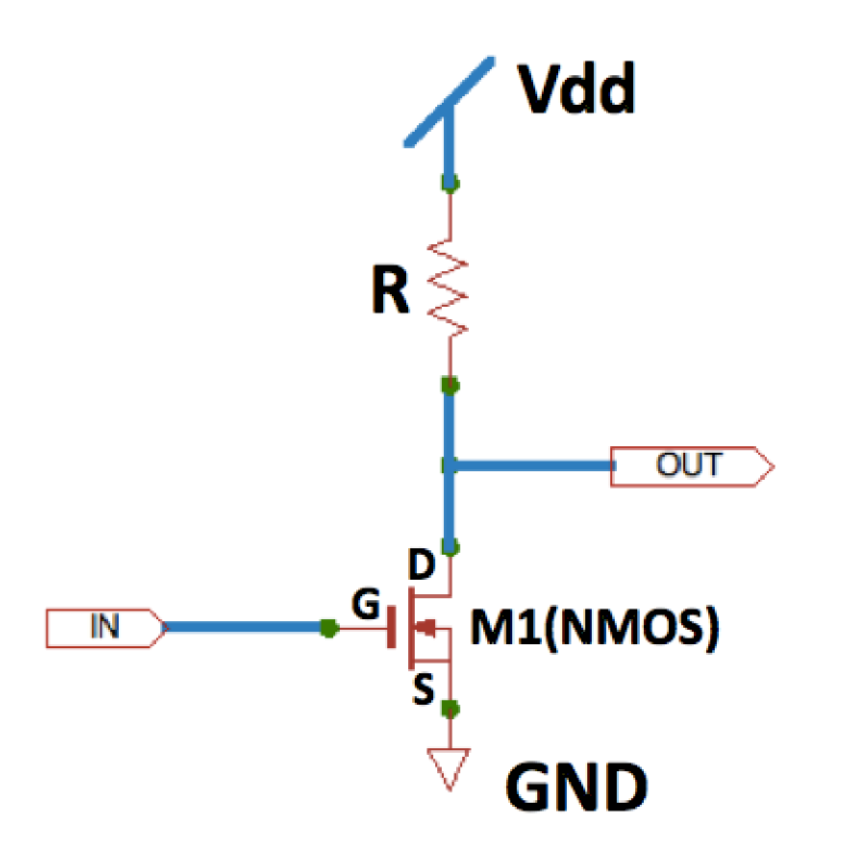
\includegraphics[width=70mm]{./Chapter/Chapter3/Picture/MOSFET_CommonSource_1.eps}
					\end{center}
					\caption{抵抗負荷を有するソース接地回路図}
					\label{fig:MOSFET_CommonSource_1}
				\end{minipage}
				\begin{minipage}{0.5\hsize}
					\begin{center}
						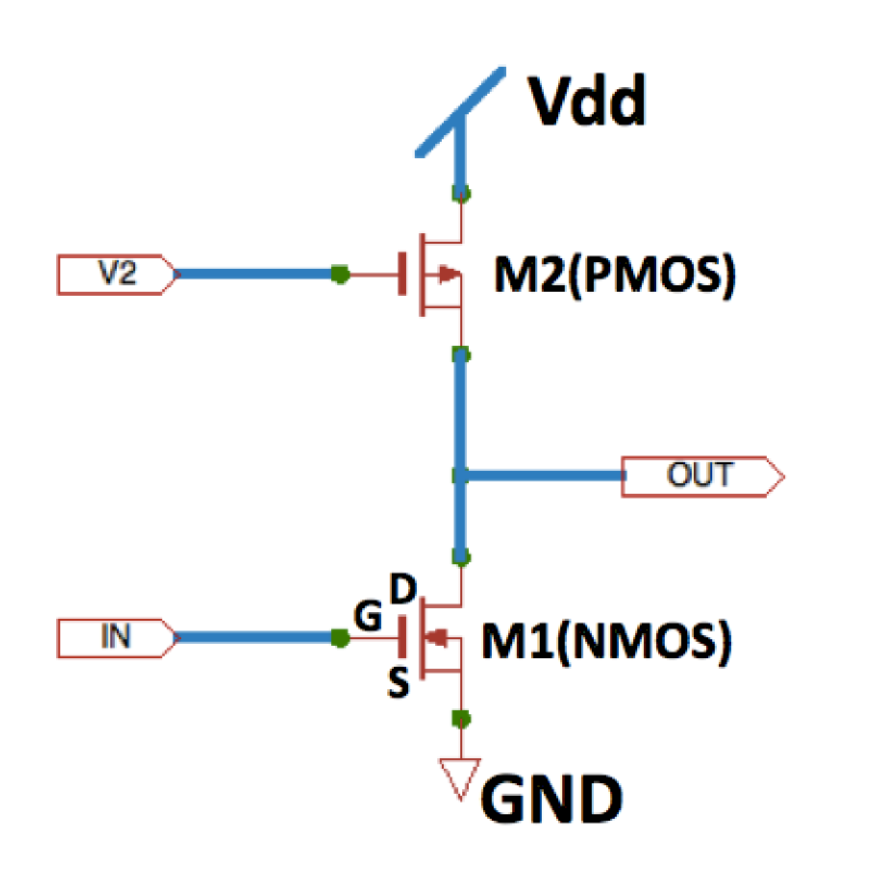
\includegraphics[width=70mm]{./Chapter/Chapter3/Picture/MOSFET_CommonSource_2.eps}
					\end{center}
					\caption{MOSFETを電流源負荷として有するソース接地回路図}
					\label{fig:MOSFET_CommonSource_2}
				\end{minipage}
			\end{figure}	
			MOSFETを用いた基本的な増幅回路として、まず「ソース接地回路」について説明する。
			図\ref{fig:MOSFET_CommonSource_1}と図\ref{fig:MOSFET_CommonSource_2}にソース接地回路図を載せる。
			まず、抵抗負荷を有する場合のソース接地回路についてに着目する。
			入力電圧($V_{IN}$)をゼロから増加させることを考える。
			はじめはM1はオフなので、M1にドレイン電流は流れない。したがって、抵抗Rでの電圧降下はないので、$V_{OUT}=V_{dd}$である。
			入力電圧$V_{IN}$が、$V_{th} + V_{OUT} > V_{IN} > V_{th}$であるとき、M1は飽和領域で動作する。
			したがって、このときの出力電圧は式{\ref{eq:MOSFET_CommonSource_1_1}}のようになる。
			ただし、ここではチャネル長変調効果を無視した。
			\begin{eqnarray}
				V_{OUT} = V_{dd} - R \frac{1}{2} \mu_e C_{OX} \frac{W}{L} {(V_{IN} - V_{th})}^2
				\label{eq:MOSFET_CommonSource_1_1}
			\end{eqnarray}
			さらに、入力電圧$V_{IN}$が、$V_{IN} > V_{OUT} + V_{th}$であるとき、M1は飽和領域を外れて線形領域で動作することになる。
			この領域において、式(\ref{eq:MOSFET_rd_linear})のようにMOSFETは抵抗のように振る舞う。
			したがって、出力電圧$V_{OUT}$は、抵抗RとMOSFETのドレイン抵抗とで抵抗分割した電圧に相当する。
			\begin{eqnarray}
				V_{OUT} = \frac{r_d (\mathrm{linear})}{rd (\mathrm{linear}) + R} V_{dd} = \frac{V_{dd}}{1 + \mu_e C_{OX} \frac{W}{L} R (V_{IN} - V_{th})}
			\end{eqnarray}
			%=====入力電圧と出力電圧の関係を示した図を載せる=====%
			\begin{figure}[htbp]
				\begin{center}
					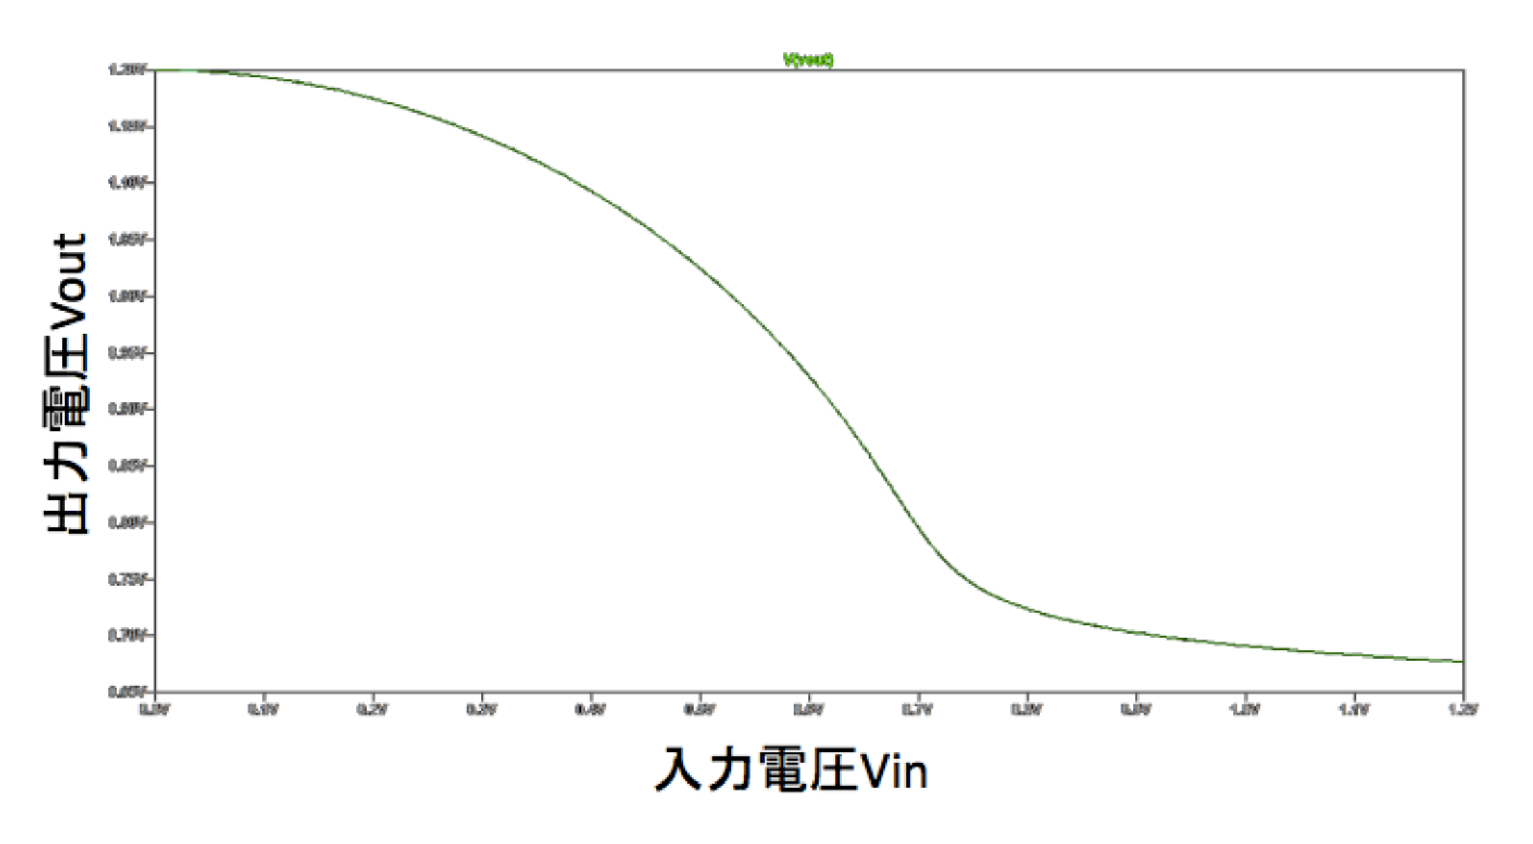
\includegraphics[width=12.0cm]{./Chapter/Chapter3/Picture/MOSFET_CommonSource_InOut.eps}
					\caption{ソース接地回路における入力電圧と出力電圧の特性}
					\label{fig:MOSFET_CommonSource_InOut}
				\end{center}
			\end{figure}
			以上より、ソース接地回路における入力電圧と出力電圧の関係性は図\ref{fig:MOSFET_CommonSource_InOut}のようになる。
			
			次に、利得について述べる。
			M1が飽和領域で動作して、かつMOSFETのチャネル長変調効果を無視しない場合、出力電圧$V_{OUT}$は式(\ref{eq:MOSFET_CommonSource_out_saturate})のように書ける。
			\begin{eqnarray}
				V_{OUT} = V_{dd} - R \frac{1}{2} \mu_e C_{OX} \frac{W}{L} {(V_{IN} - V_{th})}^2 {(1 + \lambda V_{OUT})}
				\label{eq:MOSFET_CommonSource_out_saturate}
			\end{eqnarray}
			式(\ref{eq:MOSFET_CommonSource_out_saturate})の両辺を入力電圧$V_{IN}$で微分する。
			\begin{eqnarray}
				\frac{\partial V_{OUT}}{\partial V_{IN}}
				= -R \mu_e C_{OX} \frac{W}{L} (V_{IN} - V_{th}) (1 + \lambda V_{OUT})
				- R \frac{1}{2} \mu_e C_{OX} \frac{W}{L} {(V_{IN} - V_{th})}^{2} \lambda \frac{\partial V_{OUT}}{\partial V_{IN}}
				\label{eq:MOSFET_CommonSource_out_saturate_2}
			\end{eqnarray}
			そして、$I_{ds} \approx \frac{1}{2} \mu_e C_{OX} \frac{W}{L} {(V_{IN} - V_{th})}^2$という近似を用いて、式(\ref{eq:MOSFET_CommonSource_out_saturate_2})を整理すると、電圧利得$A_{\nu}$は式(\ref{eq:MOSFET_CommonSource_out_saturate_3_1})と式(\ref{eq:MOSFET_CommonSource_out_saturate_3_2})のようになる。
			\begin{eqnarray}
				A_{\nu} & = & \frac{\partial V_{OUT}}{\partial V_{IN}} \\
				\label{eq:MOSFET_CommonSource_out_saturate_3_1}
				A_{\nu} & = & - \frac{g_m R}{1 + R \lambda I_{ds}}
				\label{eq:MOSFET_CommonSource_out_saturate_3_2}
			\end{eqnarray}
			そして、$\lambda I_{ds} = \frac{1}{r_{d} (\mathrm{saturate})}$なので、
			\begin{eqnarray}
				A_{\nu} = - g_{m} \frac{r_{d}(\mathrm{saturate}) R}{r_{d}(\mathrm{saturate}) + R}
				\label{eq:MOSFET_CommonSource_out_saturate_4}
			\end{eqnarray}
			式(\ref{eq:MOSFET_CommonSource_out_saturate_4})から、負荷抵抗Rが大きければ大きいほど電圧利得$A_{\nu}$は大きくなることがわかる。\\
			図\ref{fig:MOSFET_CommmonSource_2}にMOSFETを電流源負荷として用いたソース接地回路図を示した。
			抵抗素子の代わりにMOSFETを電流源として用いることによって、
			\begin{itemize}
				\item 一般的なCMOS技術では高精度・高抵抗な抵抗素子を形成するのは困難だが、MOSFETを用いることで高抵抗負荷を実現できる。
				\item 供給電圧を大きく消費せずに高抵抗を実現できるので、消費電力低減が期待できる。
			\end{itemize}
		\subsubsection{ソースフォロア回路}
			\begin{figure}[htbp]
				 \begin{minipage}{0.5\hsize}
					\begin{center}
						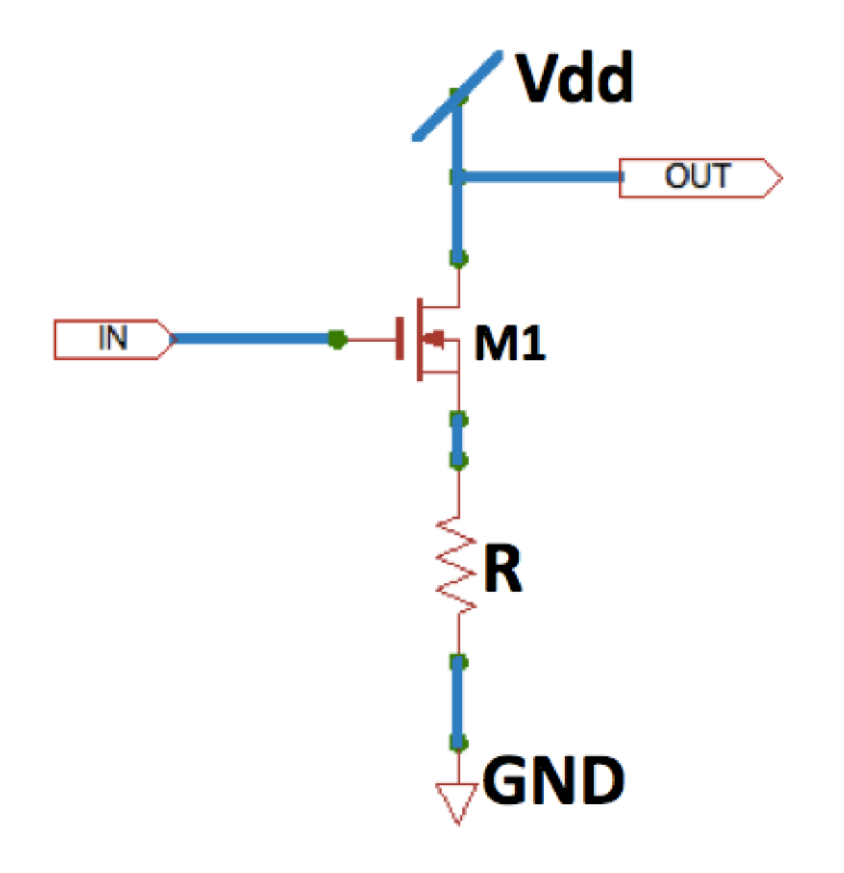
\includegraphics[width=70mm]{./Chapter/Chapter3/Picture/MOSFET_SourceFollower_1.eps}
					\end{center}
					\caption{抵抗負荷を有するソースフォロア(ドレイン接地)回路図}
					\label{fig:MOSFET_SourceFollower_1}
				\end{minipage}
				\begin{minipage}{0.5\hsize}
					\begin{center}
						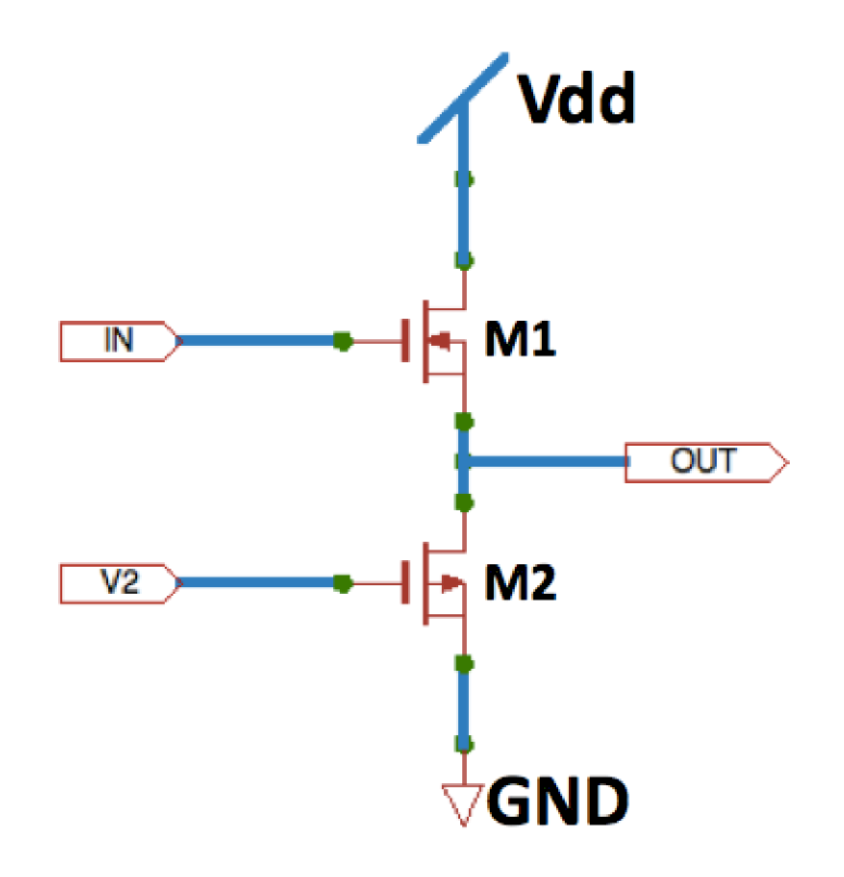
\includegraphics[width=70mm]{./Chapter/Chapter3/Picture/MOSFET_SourceFollower_2.eps}
					\end{center}
					\caption{MOSFETを電流源負荷として有するソースフォロア(ドレイン接地)回路図}
					\label{fig:MOSFET_SourceFollower_2}
				\end{minipage}
			\end{figure}	
			図\ref{fig:MOSFET_SourceFollower_1}と図\ref{fig:MOSFET_SourceFollower_2}のような回路のことをソースフォロア(ドレイン接地)回路と呼ばれる。
			前節で述べたソース接地回路において、高い電圧利得を得るためには負荷インピーダンスを大きくする必要がある。
			このような増幅段が低インピーダンスの負荷を駆動する場合は、信号電圧の損失が無視できるようにバッファを入れる必要がある。
			ソースフォロア回路は、このバッファとしての役割を果たす。\\
			%=====入力電圧と出力電圧の関係を示した図を載せる=====%
			\begin{figure}[htbp]
				\begin{center}
					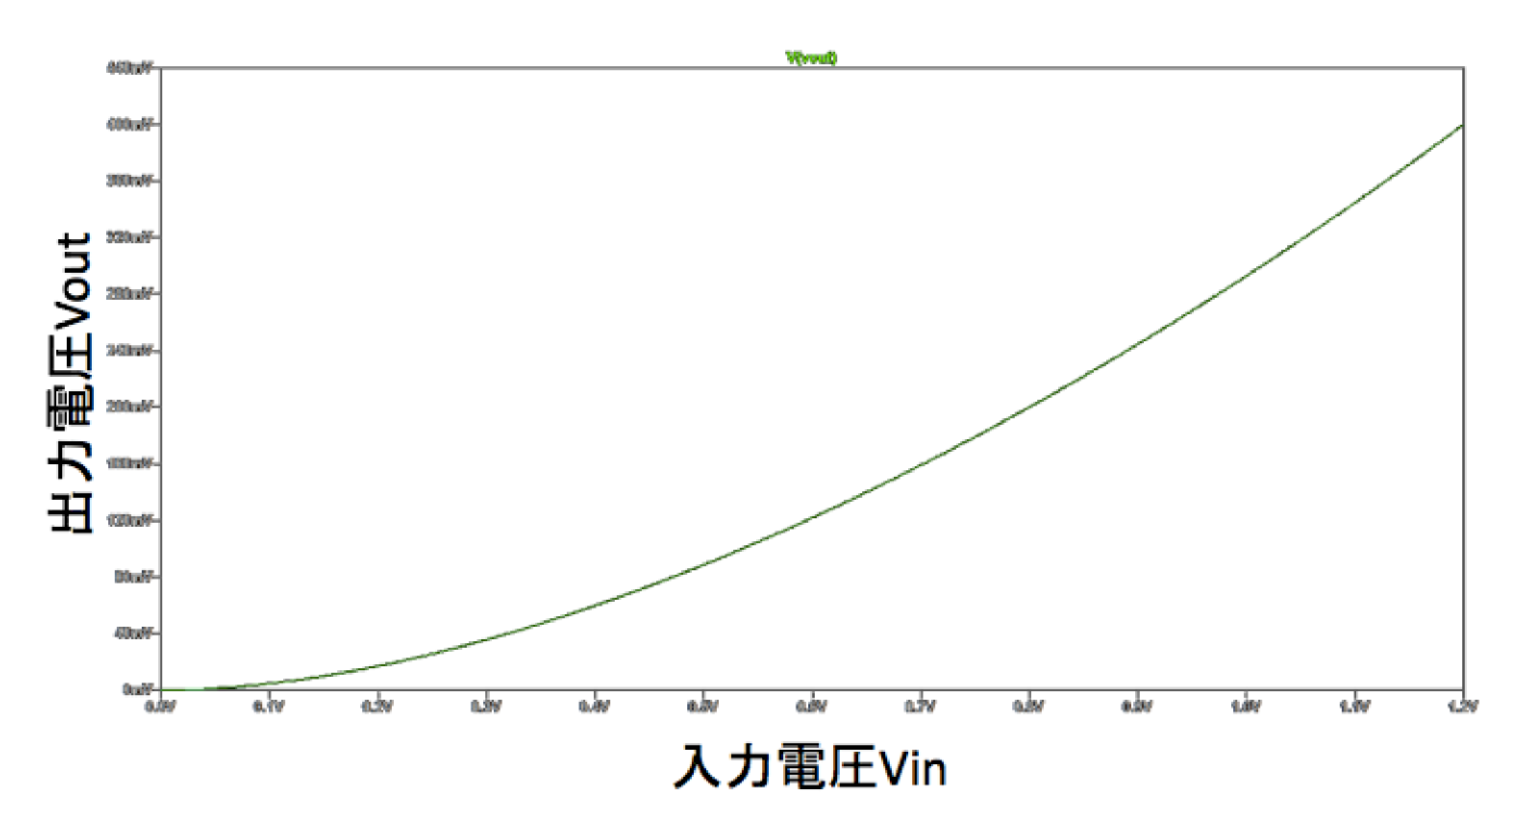
\includegraphics[width=12.0cm]{./Chapter/Chapter3/Picture/MOSFET_SourceFollower_InOut.eps}
					\caption{ソースフォロア回路における入力電圧と出力電圧の特性}
					\label{fig:MOSFET_SourceFollower_InOut}
				\end{center}
			\end{figure}
			次に前節の時と同様に、入力電圧$V_{IN}$をゼロから増加させることを考える。\\
			入力電圧$V_{IN}$が、$V_{IN} < V_{th}$ではM1はオフなので出力電圧$V_{OUT}=0$である。\\
			そして、入力電圧$V_{IN}$が、$V_{IN} > V_{OUT}$になると、M1は飽和領域で動作する
			\footnote{$V_{dd}$の値によってはM1は線形領域で動作することにもなるが、基本的にはM1は飽和領域で動作するよう$V_{dd}$を印加する。}。
			M1が飽和領域で動作していることから、ソースフォロア回路における入出力電圧の特性は式(\ref{eq:MOSFET_SourceFollower_InOut})のように書くことができる。
			\begin{eqnarray}
				V_{OUT} = \frac{1}{2} \mu_e C_{OX} \frac{W}{L} {(V_{IN} - V_{th} - V_{OUT})}^2 R
				\label{eq:MOSFET_SourceFollower_InOut}
			\end{eqnarray}
			これをグラフにすると図\ref{fig:MOSFET_SourceFollower_InOut}のようになる。\\
			次にソースフォロアの電圧利得について考える。
			式(\ref{eq:MOSFET_SourceFollower_InOut})の両辺を出力電圧$V_{IN}$で微分する。
			\begin{eqnarray}
				\frac{\partial V_{OUT}}{\partial V_{IN}} = \frac{1}{2} \mu_e C_{OX} \frac{W}{L} 2 (V_{IN} - V_{th} - V_{OUT}) \left( 1 - \frac{\partial V_{th}}{\partial V_{IN}} \right) R
				\label{eq:MOSFET_SourceFollower_1}
			\end{eqnarray}
			そして、
			\begin{eqnarray}
				\frac{\partial V_{th}}{\partial V_{IN}} = \eta \frac{\partial V_{OUT}}{\partial V_{IN}}
			\end{eqnarray}
			であることから、電圧利得$A_{\nu}$は式(\ref{eq:MOSFET_SourceFollower_2_1})と式(\ref{eq:MOSFET_SourceFollower_2_2})のようになる。
			\begin{eqnarray}
				A_{\nu} & = & \frac{\partial V_{OUT}}{\partial V_{IN}} \\
				\label{eq:MOSFET_SourceFollower_2_1}
				A_{\nu} & = & \frac{\mu_e C_{OX} \frac{W}{L} (V_{IN} - V_{th} - V_{OUT}) R}{1 + \mu_e C_{OX} \frac{W}{L} (V_{IN} - V_{th} - V_{OUT}) R (1 + \eta)}
				\label{eq:MOSFET_SourceFollower_2_2}
			\end{eqnarray}
			トランスコンダクタンス$g_m$は、
			\begin{eqnarray}
				g_m = \mu_e C_{OX} \frac{W}{L} (V_{IN} - V_{th} - V_{OUT})
			\end{eqnarray}
			であることから、トランスコンダクタンスが大きいほど増幅率は1に近づく。
			そしてソースフォロア回路はソース接地回路と同様に負荷抵抗の代わりにMOSFETを電流源として用いる。
			\clearpage
\section{SOI-MOSFET}
	前節まではMOSFETの電気的特性やMOSFETを用いた基本的な増幅回路について述べた。
	本節ではMOSFETの構造について、まず一般的なBulk-CMOSの構造について述べる。
	Bulk-CMOSとはシリコンSiバルク上にMOSFETが形成された構造を呼ぶ。
	
	対して、SOI(Silicon On Insulator)-MOSFETと呼ばれるMOSFETがある。これは$\mathrm{SiO_2}$酸化膜上に形成されたMOSFETである。\\
	このSOI-MOSFETの中でもチャネル層が非常に薄く形成されたFD(Fully Depleted)-SOI-MOSFETは4Kで動作したことが確認されている。\\
	本節ではこのSOI-MOSFETの極低温特性についても詳しく述べる。
	\subsection{CMOS}
		\begin{figure}[htbp]
			\begin{center}
				\includegraphics[width=12.0cm]{./Chapter/Chapter3/Picture/CMOS_structure.eps}
				\caption{Bulk-CMOSの構造}
				\label{fig:CMOS_structure}
			\end{center}
		\end{figure}
		1つの基板上に複数のMOSFETを集積して組み合わせた構造のことをCMOS(Complementary MOS)と呼ばれる。
		通常のBulk CMOSは基板とデバイス同士がPN接合の逆バイアス電圧によって分離される。
		Bulk-CMOSの構造は図\ref{fig:CMOS_structure}に示した。
		
		しかしこれでは素子同士の分離は完全ではない。
		SOIプロセスで形成されたMOSFETでは、より素子同士の分離が完全になる。
		
	\subsection{PD-SOI-FETとFD-SOI-FET}
		\begin{figure}[htbp]
			\begin{center}
				\includegraphics[width=12.0cm]{./Chapter/Chapter3/Picture/SOIFET_structure.eps}
				\caption{SOI-CMOSの構造(左 : FD-SOI-MOSFET    右 : PD-SOI-MOSFET)}
				\label{fig:SOIFET_structure}
			\end{center}
		\end{figure}
		SOIプロセスによって形成されたMOSFETは素子同士を絶縁膜である$\mathrm{SiO_2}$で完全に電気的に分離する。
		
		我々のCOBAND実験において、Bulk-CMOSよりもSOI-CMOSの方が優れている点として以下の3点が挙げられる。
		\begin{description}
			\item[集積化に非常に優れている]\mbox{}\\
				絶縁膜により素子を完全に電気的に分離しているので、素子間のクロストークが非常に小さいので集積化に優れている。
			\item[低消費電力化が可能]\mbox{}\\
				Bulk-CMOSの場合、基板と各端子間との寄生容量が生じてしまう。
				対してSOI-CMOSの場合はそれに起因する寄生容量を抑えることができる。
			\item[回路の高速化が可能]\mbox{}\\
				前述と同様、寄生容量を抑えられるので、低消費電力化と同時に高速化も期待される。
		\end{description}
		そしてSOI-MOSFETは、ゲート直下のチャネル層の厚みにより、
		\begin{description}
		\item[部分空乏型SOI(PD-SOI : Partially Depleted SOI)]\mbox{}\\
			SOI層の厚みはおよそ100nm〜200nm程度。\\
			チャネル層が厚いのでゲート電圧を印加してもゲート直下のみが部分的に空乏化され、電気的に中性な領域(Body)が現れる。
		\item[完全空乏型SOI(FD-SOI : Fully Depleted SOI)]\mbox{}\\
			SOI層の厚みは50nm以下でPD-SOIプロセスで形成されてMOSFETよりも非常に薄い。\\
			チャネル層が薄いのでゲート直下のシリコン層は完全に空乏化する。
		\end{description}
		に大別される。
		
		特にFD-SOIプロセスで形成されたMOSFETは浮遊帯効果を抑制でき、我々が極低温環境下で動作させるのに最大のメリットが発揮される。
		
		浮遊帯効果とはMOSFETが動作している際、そのキャリアの衝突イオン化により生成された正孔がBody部分に蓄積し、結果Body電位が変化するのでMOSFETが誤作動を起こしてしまう効果のことである。
		低温環境下においてキャリア移動度が上昇するので、この衝突イオン化が起こりやすくなる。
		したがって、極低温環境下でMOSFETを用いることを考える場合は浮遊帯効果を抑制できるようなMOSFETを用いる必要がある。
		この浮遊体効果はBulk-CMOSプロセスで形成されたMOSFETはもちろん、PD-SOIプロセスで形成されたMOSFETも浮遊帯効果により低温環境下では動作しない。
		
		しかし、FD-SOI-MOSFETはbody部分が完全に空乏化されるので浮遊帯効果は起こらない。実際、JAXAはFD-SOI-MOSFETが4Kで動作したことを確認した\cite{6}。
	\subsection{極低温特性}
		\begin{figure}[htbp]
			\begin{minipage}{0.5\hsize}
				\begin{center}
					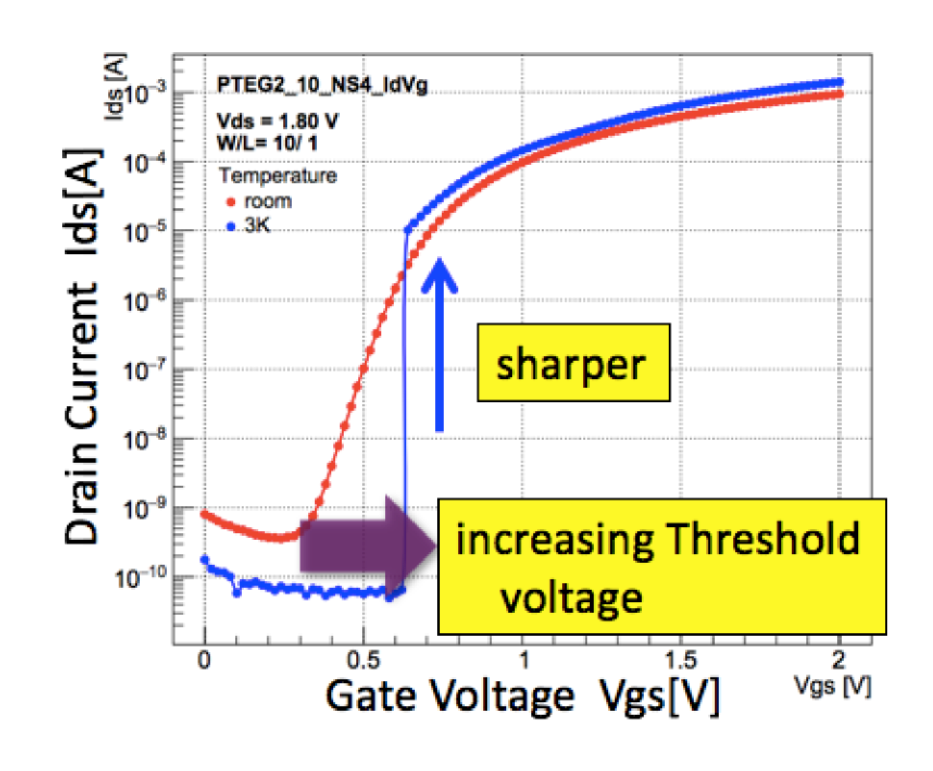
\includegraphics[width=60mm]{./Chapter/Chapter3/Picture/MOSFET_IdVg_temp.eps}
				\end{center}
				\caption{FD-SOI-MOSFETのドレイン電流の温度依存性($I_{ds} - V_{gs}$特性)}
				\label{fig:MOSFET_IdVg_temp}
			\end{minipage}
			\begin{minipage}{0.5\hsize}
				\begin{center}
					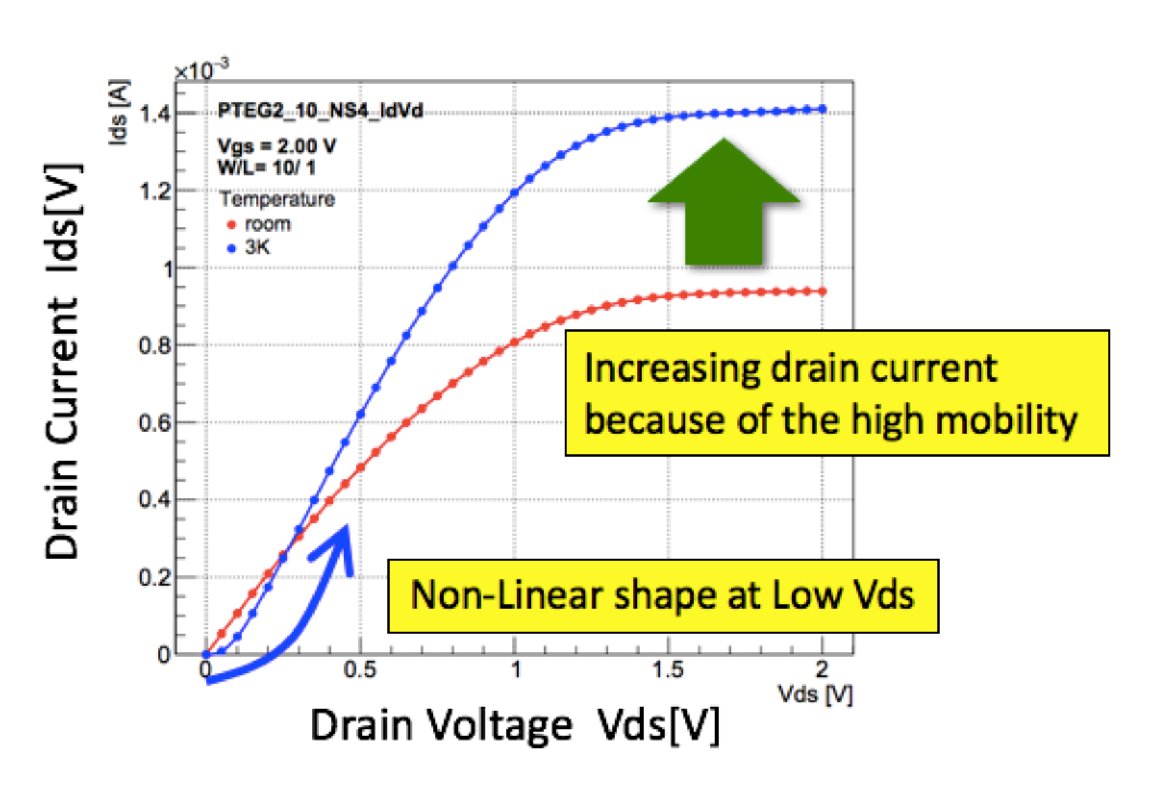
\includegraphics[width=80mm]{./Chapter/Chapter3/Picture/MOSFET_IdVd_temp.eps}
				\end{center}
				\caption{FD-SOI-MOSFETのドレイン電流の温度依存性($I_{ds} - V_{ds}$特性)}
				\label{fig:MOSFET_IdVd_temp}
			\end{minipage}
		\end{figure}
		FD-SOI-MOSFETのドレイン電流の温度依存性について、図\ref{fig:MOSFET_IdVg_temp}と図\ref{fig:MOSFET_IdVd_temp}に示した。
		室温時(赤点)のMOSFETの電流電圧特性と3K時(青点)のMOSFETの電流電圧特性を比較すると、極低温環境下では、
		\begin{itemize}
			\item 閾電圧の上昇
			\item サブスレッショルド領域で立ち上がりがより鋭くなる
			\item キャリア移動度上昇による飽和電流値の上昇
		\end{itemize}
		が見られる。ただし、3K環境下と300mK環境下ではFD-SOI-MOSFETの電流電圧特性の基本動作に変化はない。
		さらに、極低温環境下におけるドレイン電流のドレイン電圧特性($I_{ds}-V_{ds}$特性)に着目すると、以下のような異常特性が確認されている。
		\begin{itemize}
			\item $V_{ds}$が高い領域でドレイン電流の急激な上昇(Kink効果)
			\item $V_{ds}$が低い領域でのドレイン抵抗の異常な上昇
		\end{itemize}
		上記1つ目の異常特性によって、Kink効果が現れない電圧に調整することで異常特性を回避することができる。
		上記2つ目の異常特性に関してはLDD不純物濃度を濃くすることによって改善できることを確認しており、これは次章で詳しく報告する。
		
		以上のように、極低温環境下におけるFD-SOI-MOSFETの電流電圧特性は常温環境下から大きく変化するので、これらの特性変動を踏まえた上で極低温環境用の増幅器開発をする必要がある。
		\clearpage
		
\section{極低温増幅器への要求}
	我々はFD-SOI-MOSFETを用いた極低温環境用前置増幅器でNb/Al-STJ検出器信号の増幅を行う。その前置増幅器には以下の要求が課される。
	\begin{description}
		\item[Nb/Al-STJ検出器信号のような高速な信号でも増幅可能であること]\mbox{}\\
			STJ検出器の信号幅は数$\mathrm{\mu s}$から数百$\mathrm{\mu s}$程度である。
			したがって数十kHzから数MHz帯域の信号に対しても十分増幅できる回路である必要がある。
		\item[冷凍機配線容量を駆動可能]\mbox{}\\
			冷凍機配線は常温環境下からサンプルが設置された極低温環境下へ熱アンカーを取るため非常に長い。
			したがって、冷凍機の配線容量は数百pF程度で非常に大きいことが確認されている。
		\item[極低温環境下でも増幅器として動作可能であること]\mbox{}\\
			現在我々が性能評価を行っているCRAVITY製Nb/Al-STJ検出器のリーク電流は約400mK程度で下げ止まる。
			STJ検出器直近で動作させる場合は400mK以下でも動作可能な増幅器である必要がある。
		\item[400チャンネルに対して消費電力が$0.25\mathrm{W}$以下であること]\mbox{}\\
			次章で述べるが、我々が用いる冷凍機の冷却能力は350mKで100$\mathrm{\mu W}$程度である。
			もし増幅器をSTJ検出器直近で動作させる場合は、増幅器の消費電力は100$\mu W$以下である必要がある。
			しかし、現在極低温環境用前置増幅器の設計において、350mKでの消費電力の要求は非常に厳しいのが現状である。
			もし増幅器をより冷却能力が高い3K環境に設置する場合、400チャンネルに対する消費電力への要求は0.25$\mathrm{W}$に軽減される。
	\end{description}
	以上の要求を満たすように我々はFD-SOI-MOSFETを用いた極低温環境用増幅器(以下、SOI増幅器と呼ぶ)の研究開発を行ってきた。
	次節から、極低温環境用前置増幅器の研究開発の現状について順を追って述べる。
	\clearpage
\section{極低温環境用SOI前置増幅器の研究開発の現状}
	現時点では、極低温環境用SOI-MOSFETのSPICE回路シミュレーターは完成していないので、前置増幅器の設計は常温環境下でのSOI-MOSFETのパラメータで行い、極低温環境下で動作させる時に各MOSFETの極低温特性を考慮し電圧設定を決定した。
	\subsection{SOI前置増幅器一体型STJ検出器}
		\begin{figure}[htbp]
			\begin{center}
				\includegraphics[width=12.0cm]{./Chapter/Chapter3/Picture/SOISTJ_structure.eps}
				\caption{SOI前置増幅器一体型STJ検出器(SOI-STJ)の構造概念図}
				\label{fig:SOISTJ_structure}
			\end{center}
		\end{figure}
		前章で、STJ検出器が動作する極低温環境下においても動作可能な前置増幅器を冷凍機内に設置し、STJ検出器信号が冷凍機の長い配線を経て読み出す際に生じる雑音に埋もれる前に増幅させるようと考えていることを述べた。
		出来るだけSOI増幅器をSTJ検出器に近づければ、冷凍機配線に起因する測定系雑音の影響を回避して増幅することができる。
		究極的にはSOI増幅器回路基板上にSTJ検出器を直接形成した増幅器と検出器が一体型の光検出器にすることで、冷凍機配線を介さずに増幅することが出来るので、SN比がよくなることが期待される。\\
		図\ref{fig:SOISTJ_structure}にSOI前置増幅器とSTJ検出器が一体型となった光検出器(SOI-STJ)の構造概念図を示す。SOI回路基板上に直接STJ検出器を形成している。
		回路との電気的接触はタングステンのビアを介して行われており、また回路基板の表面はCMP研磨によって平坦化を行う。\\
		SOI回路基板は株式会社ラピスセミコンダクタに制作を依頼している。
	\subsection{1号機(SOI-STJ1)}
		\begin{figure}[htbp]
			\begin{center}
				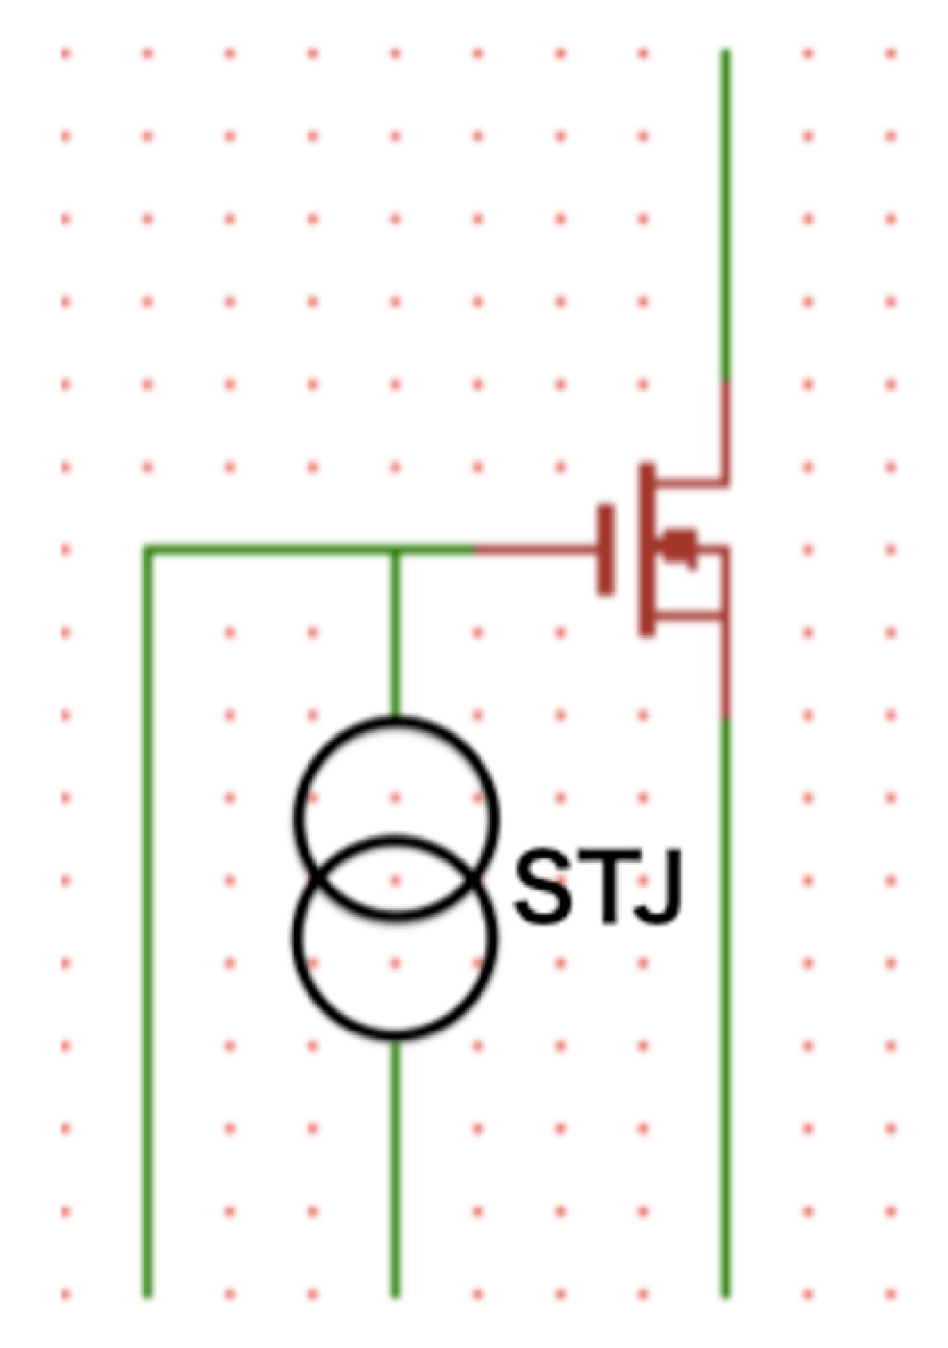
\includegraphics[width=6.0cm]{./Chapter/Chapter3/Picture/SOISTJ1_circuit.eps}
				\caption{極低温環境用SOI前置増幅器1号機(SOI-STJ1)}
				\label{fig:SOISTJ1_circuit}
			\end{center}
		\end{figure}
		試作段階として2013年度にSOI増幅器1号機(以下、SOI-STJ1)が制作された。SOI-STJ1の回路図を図\ref{fig:SOISTJ1_circuit}に示す。
		またSOI-STJ1ではFETの型に応じて2パターンの回路を用意している。それぞれの詳細については表\ref{tab:SOISTJ1_detail}に示す。
		\begin{table}[htb]
			\begin{center}
				\begin{tabular}{| l || c | c | c | c |} \hline
					\  & FET Type & Channel Width & Channel Length & Gate Cap. \\ \hline \hline
					Pattern1 & Nch & $10\mathrm{\mu m} \times 100$ & $1 \mathrm{\mu m}$ & $8 \mathrm{pF}$ \\ \hline
					Pattern2 & Pch & $10\mathrm{\mu m} \times 100$ & $1 \mathrm{\mu m}$ & $8 \mathrm{pF}$ \\ \hline
				\end{tabular}
				\caption{SOI-STJ1の各パターンごとのFETの詳細}
				\label{tab:SOISTJ1_detail}
			\end{center}
		\end{table}
		SOI回路基板上にNb/Al-STJ検出器を形成したSOI-STJ1の性能評価実験によって以下の結果が得られた。
		\begin{enumerate}
			\item SOI回路基板にNb/Al-STJ検出器を形成しても、Nb/Al-STJは損傷はなく正常に動作した。
			\item SOI-MOSFETがNb/Al-STJの動作温度(1K以下)でも正常に動作した。
		\end{enumerate}
	\subsection{2号機(SOI-STJ2)}
		\begin{figure}[htbp]
			\begin{center}
				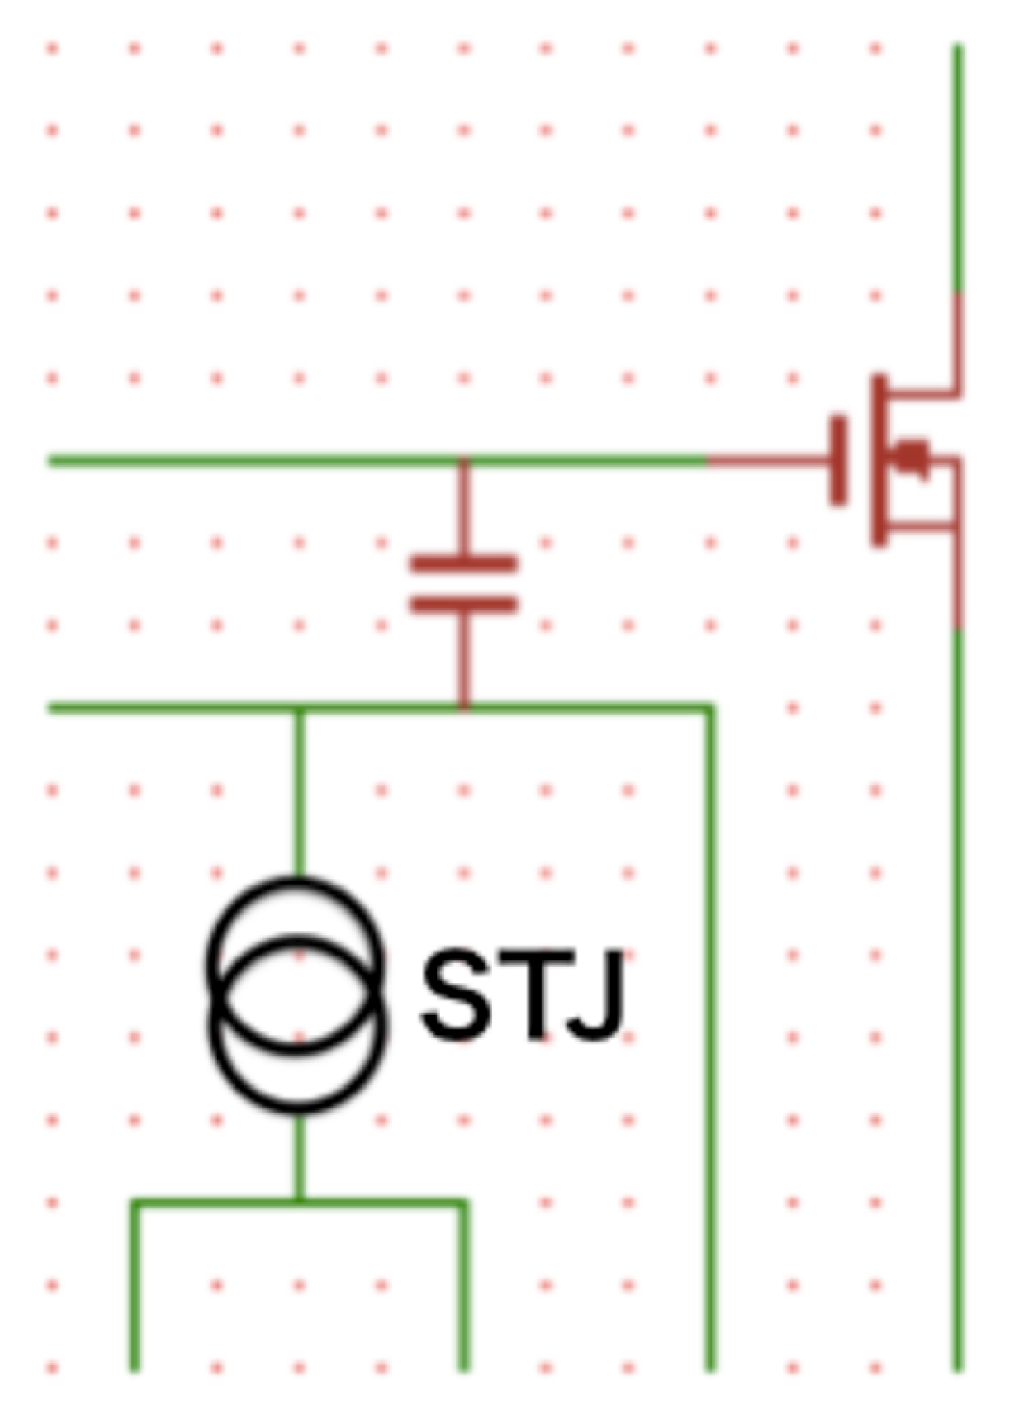
\includegraphics[width=6.0cm]{./Chapter/Chapter3/Picture/SOISTJ2_circuit.eps}
				\caption{極低温環境用SOI前置増幅器2号機(SOI-STJ2)}
				\label{fig:SOISTJ2_circuit}
			\end{center}
		\end{figure}
		SOI-STJ1では、以下のような問題点があった。
		\begin{enumerate}
			\item FETのゲート電圧とSTJ検出器のバイアス電圧を独立に印加することができない。
			\item 形成されているFETのゲートキャパシタンスが非常に大きいのでSTJ信号に対する電圧変動が小さい。
			\item ゲートキャパシタンスが大きいことから、同時に周波数応答も悪化する。
		\end{enumerate}
		以上の問題を解決するために、SOI-STJ2が制作された。\\
		図\ref{fig:SOISTJ2_circuit}にSOI-STJ2の回路図を示す。SOI-STJ1での問題解決のために以下の2つを変更した。
		\begin{enumerate}
			\item キャパシタンスを導入することによって、FETのゲート電圧とSTJ検出器のバイアス電圧を独立に印加できるようにした
			\item ゲートキャパシタンスを小さくするために、FETのサイズを小さくした。
		\end{enumerate}
		SOI-STJ2でもSTJが動作する温度(1K以下)でも正常に動作することを確認した。
		実際SOI-STJ2の性能を図\ref{fig:SOISTJ2_chara}に示す。
		\begin{figure}[htbp]
			\begin{center}
				\begin{tabular}{c}
					\begin{minipage}{0.5\hsize}
						\begin{center}
							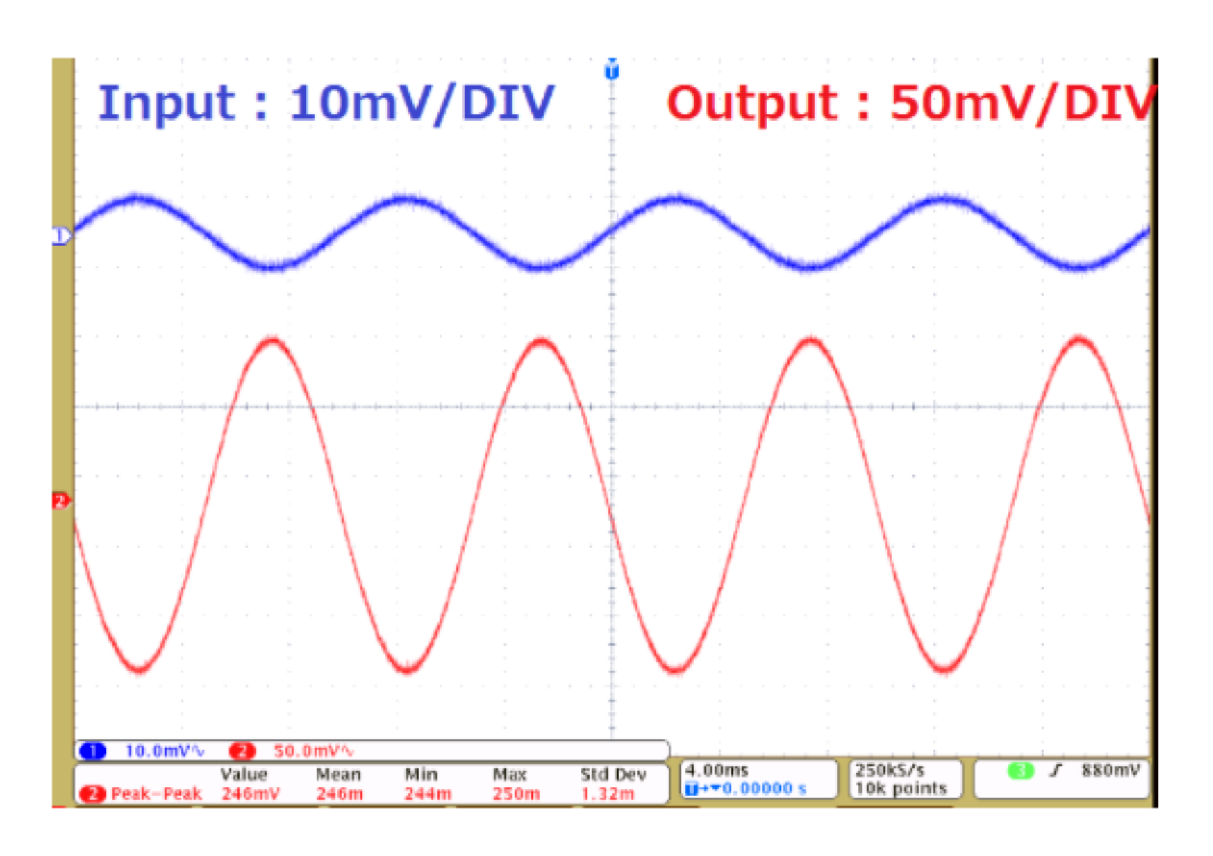
\includegraphics[clip, width=7.0cm]{./Chapter/Chapter3/Picture/SOISTJ2_InOut.eps}
							\hspace{1.6cm} [a] 入出力電圧の関係
						\end{center}
					\end{minipage}
					\begin{minipage}{0.5\hsize}
						\begin{center}
							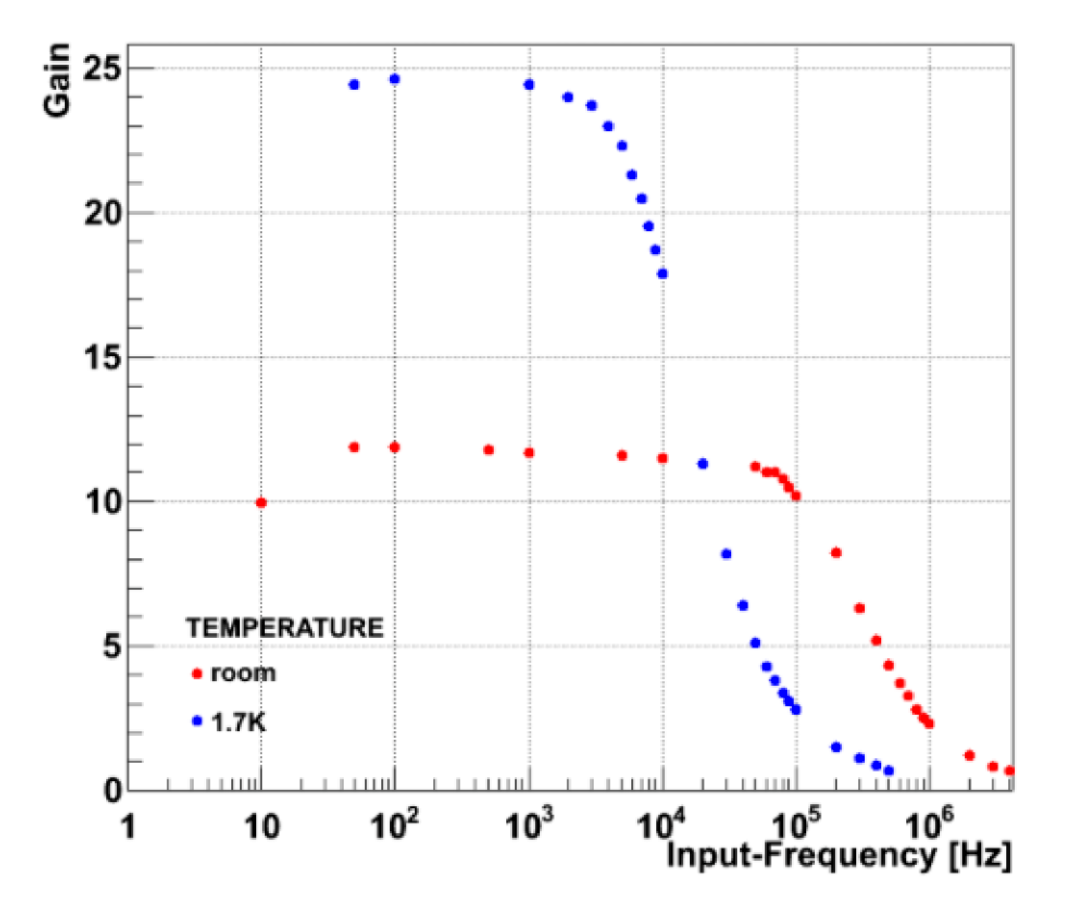
\includegraphics[clip, width=7.0cm]{./Chapter/Chapter3/Picture/SOISTJ2_frequency.eps}
							\hspace{1.6cm} [b] 周波数特性(赤点 : 室温  青点 : 1.7K)
						\end{center}
					\end{minipage}
				\end{tabular}
				\caption{SOI-STJ2の極低温環境下での性能評価}
				\label{fig:SOISTJ2_chara}
			\end{center}
		\end{figure}
		図\ref{fig:SOISTJ2_chara}[a]にSOI-STJ2のソース接地増幅回路における入出力波形を示した。これによると、電圧利得は約25程度獲得できていることが確認できる。
		また図\ref{fig:SOISTJ2_chara}[b]には周波数特性を示した。これによると極低温環境下において入力周波数$1\mathrm{kHz}$程度までは安定して動作していることを確認できる。
		
		これらの結果を踏まえ、SOI-STJ2に新たな問題点が浮上する。
		\begin{description}
			\item[電圧利得が十分ではない]\mbox{}\\
				SOI-STJ2でソース接地増幅回路を組む場合、負荷抵抗を冷凍機配線を介して導入する。
				前述のように電圧利得が十分ではない場合、負荷抵抗を大きくすることでより大きな電圧利得を獲得することができる。
				しかし、それに伴い供給電圧も大きくなり、結果それがMOSFETの耐電圧を超えてしまい素子破壊につながる危険性がある。
			\item[STJ検出器信号速度まで安定して増幅できない]\mbox{}\\
				ソース接地増幅回路のみでは出力インピーダンスが高く、高周波数帯での応答が得られない。
		\end{description}
		
		以上の問題を解決するためにSOI-STJ3の設計が行われた。
		\begin{table}[htb]
			\begin{center}
				\begin{tabular}{| c || c | c | c | c | c |} \hline
					\  & FET Type & Cap. & Channel Width & Channel Length & Gate Cap. \\ \hline \hline
					Pattern1 & Nch & 60pF & $4\mathrm{\mu m} \times 10$ & $1 \mathrm{\mu m}$ & $320 \mathrm{fF}$ \\ \hline
					Pattern2 & Pch & 60pF & $4\mathrm{\mu m} \times 10$ & $1 \mathrm{\mu m}$ & $320 \mathrm{fF}$ \\ \hline
					Pattern3 & Nch & 18pF & $1\mathrm{\mu m} \times 4$ & $1 \mathrm{\mu m}$ & $32 \mathrm{fF}$ \\ \hline
					Pattern4 & Pch & 18pF & $1\mathrm{\mu m} \times 4$ & $1 \mathrm{\mu m}$ & $32 \mathrm{fF}$ \\ \hline
					Pattern5 & Nch & 1.5pF & $1.42\mathrm{\mu m}$ & $0.4 \mathrm{\mu m}$ & $4.5 \mathrm{fF}$ \\ \hline
					Pattern6 & Pch & 1.5pF & $1.42\mathrm{\mu m}$ & $0.4 \mathrm{\mu m}$ & $4.5 \mathrm{fF}$ \\ \hline
				\end{tabular}
				\caption{SOI-STJ2の各パターンごとのFETの詳細}
				\label{tab:SOISTJ2_detail}
			\end{center}
		\end{table}
		\clearpage
	\subsection{3号機(SOISTJ-3)}
		\begin{figure}[htbp]
			\begin{center}
				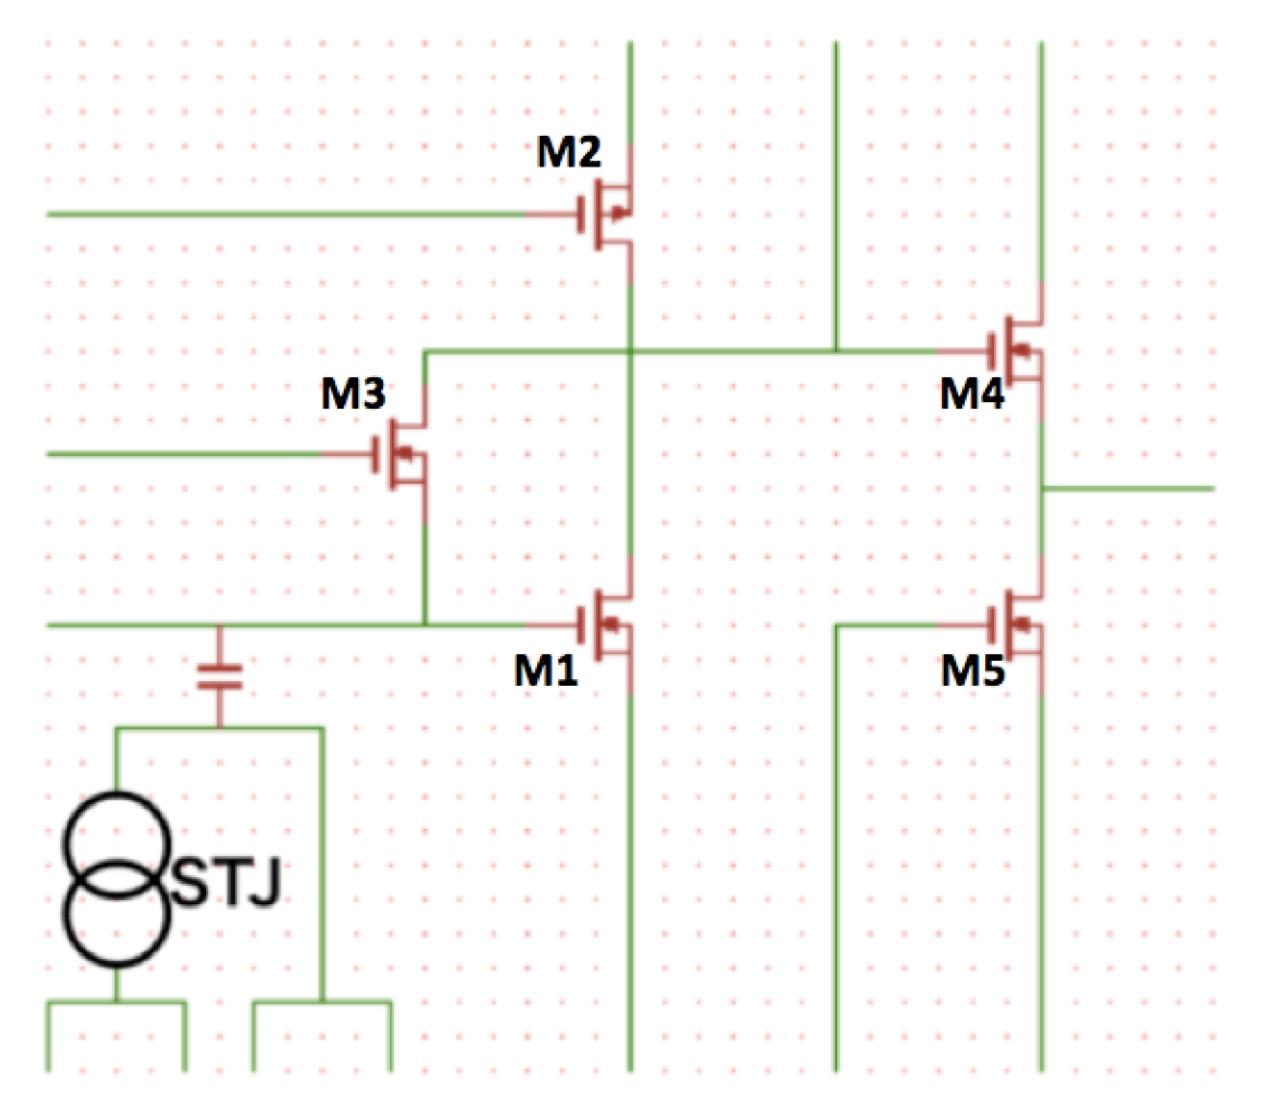
\includegraphics[width=8.0cm]{./Chapter/Chapter3/Picture/SOISTJ3_circuit.eps}
				\caption{極低温環境用SOI前置増幅器3号機(SOI-STJ3)}
				\label{fig:SOISTJ3_circuit}
			\end{center}
		\end{figure}
		\begin{table}[htb]
			\begin{center}
				\begin{tabular}{| c | c | c | c |} \hline
					FET ID & FET Type & Channel Width & Channel Length \\ \hline \hline
					M1 & N\ ch & $2.9 \mathrm{\mu m}$ & $1 \mathrm{\mu m}$ \\ \hline
					M2 & P\ ch & $1 \mathrm{\mu m}$ & $5 \mathrm{\mu m}$ \\ \hline
					M3 & N\ ch & $1 \mathrm{\mu m}$ & $2 \mathrm{\mu m}$ \\ \hline
					M4 & N\ ch & $60 \mathrm{\mu m}$ & $1 \mathrm{\mu m}$ \\ \hline
					M5 & N\ ch & $70 \mathrm{\mu m}$ & $1 \mathrm{\mu m}$ \\ \hline
				\end{tabular}
				\caption{SOI-STJ3に形成されているMOSFETの詳細}
				\label{tab:SOISTJ3_detail}
			\end{center}
		\end{table}
		SOI-STJ2での問題点解決のために、新たにSOI-STJ3を設計した。回路図を図\ref{fig:SOISTJ3_circuit}に示す。
		問題解決のために、以下の変更を行った。
		\begin{enumerate}
			\item NMOS(M3)の導入
			\item PMOS(M2)の導入
			\item ソースフォロアによるバッファ回路(M4とM5)の導入
		\end{enumerate}
		以下、各変更点についての詳細について述べる。
		\begin{description}
			\item[変更点1]\mbox{}\\
				M3を導入することによって、これは増幅段に用いるM1のゲート・ドレイン間の可変抵抗として動作する。
				これによって、M1をソース接地増幅回路として動作させるための適切なゲート電圧とドレイン電圧を設定することができる。
			\item[変更点2]\mbox{}\\
				SOI-STJ2ではソース接地回路としてMOSFETを動作させるために外部から負荷抵抗を導入した。しかし実際には十分な電圧利得を得られていないのが現状である。
				前述の通り負荷抵抗を大きくしすぎると、MOSFETの耐電圧を超える供給電圧が必要になってしまう。
				そこで、負荷抵抗の代わりにMOSFETを電流源負荷として使用するためにM2を導入した。
			\item[変更点3]\mbox{}\\
				SOI-STJ2では出力インピーダンスが非常に大きくなってしまうので、ソースフォロア回路を導入した
		\end{description}
		しかし、今までの増幅器設計の際にSTJ検出器の静電容量を考慮していなかった。
		STJ検出器の静電容量は数十から数百pF程度であるのに対し、SOI-STJ3に形成されたキャパシタンスは数十pF程度である。
		この場合検出器側に比べ増幅回路側のインピーダンスが非常に大きい設計であり、結果図\ref{fig:SOISTJ3_problem}のようにSTJ信号が回路側に伝送されない。\\
		この問題を解決するためにSOI-STJ4の設計を行った。
		\begin{figure}[htbp]
			\begin{center}
				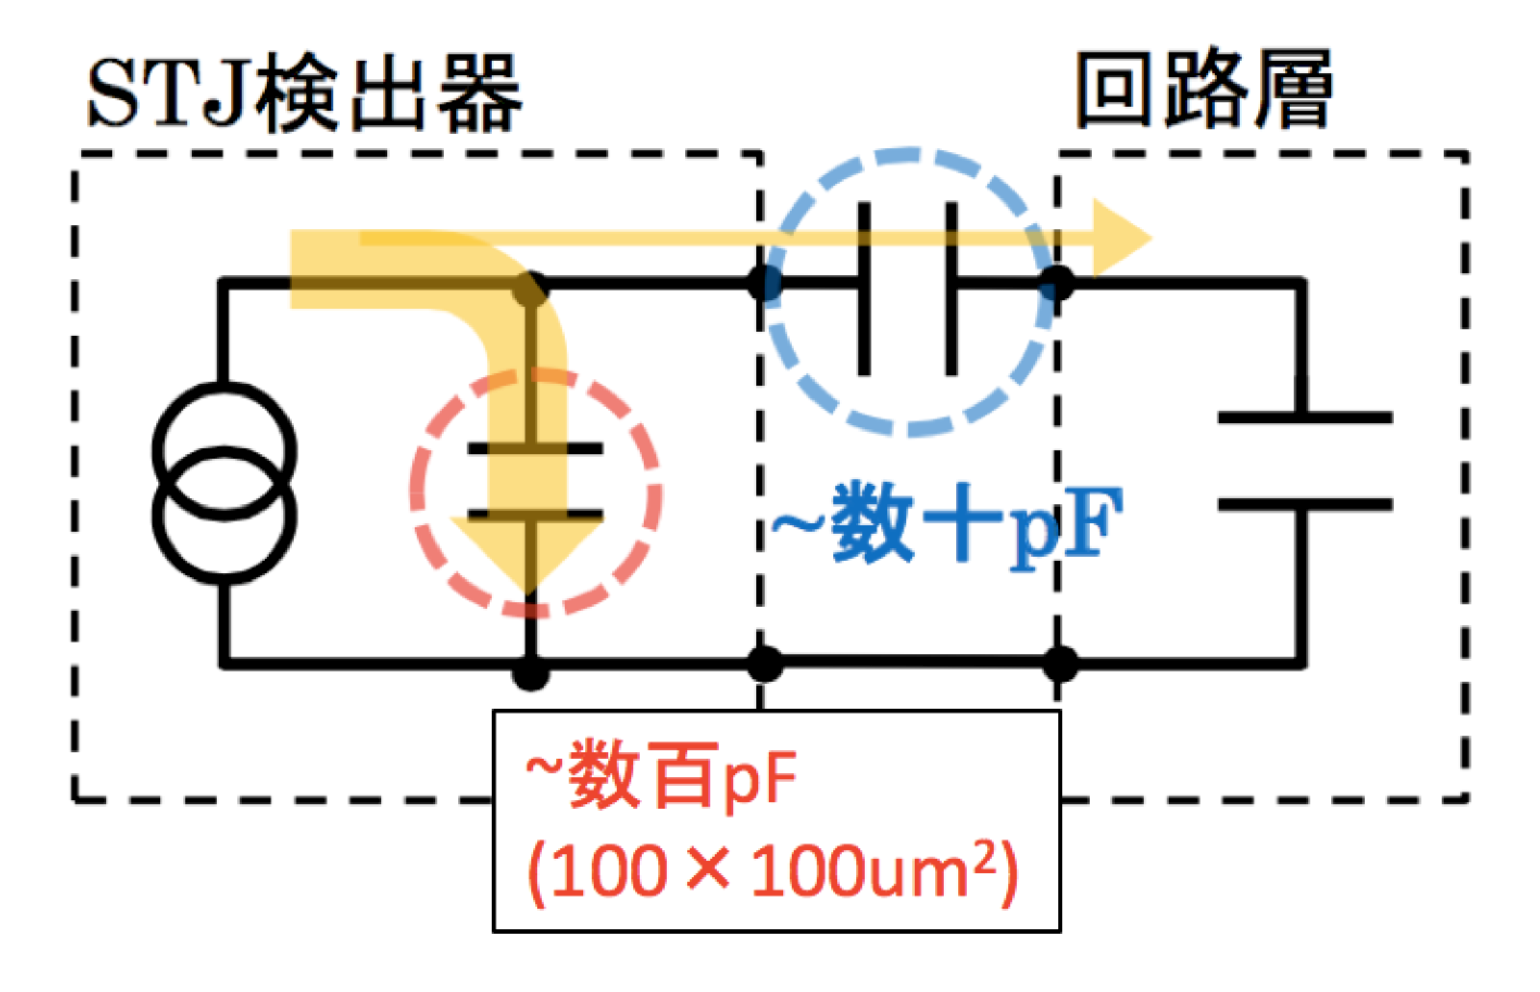
\includegraphics[width=10.0cm]{./Chapter/Chapter3/Picture/SOISTJ3_problem.eps}
				\caption{SOI-STJ3の問題点}
				\label{fig:SOISTJ3_problem}
			\end{center}
		\end{figure}
		\clearpage
	\subsection{4号機(SOI-STJ4)}
		\begin{figure}[htbp]
			\begin{center}
				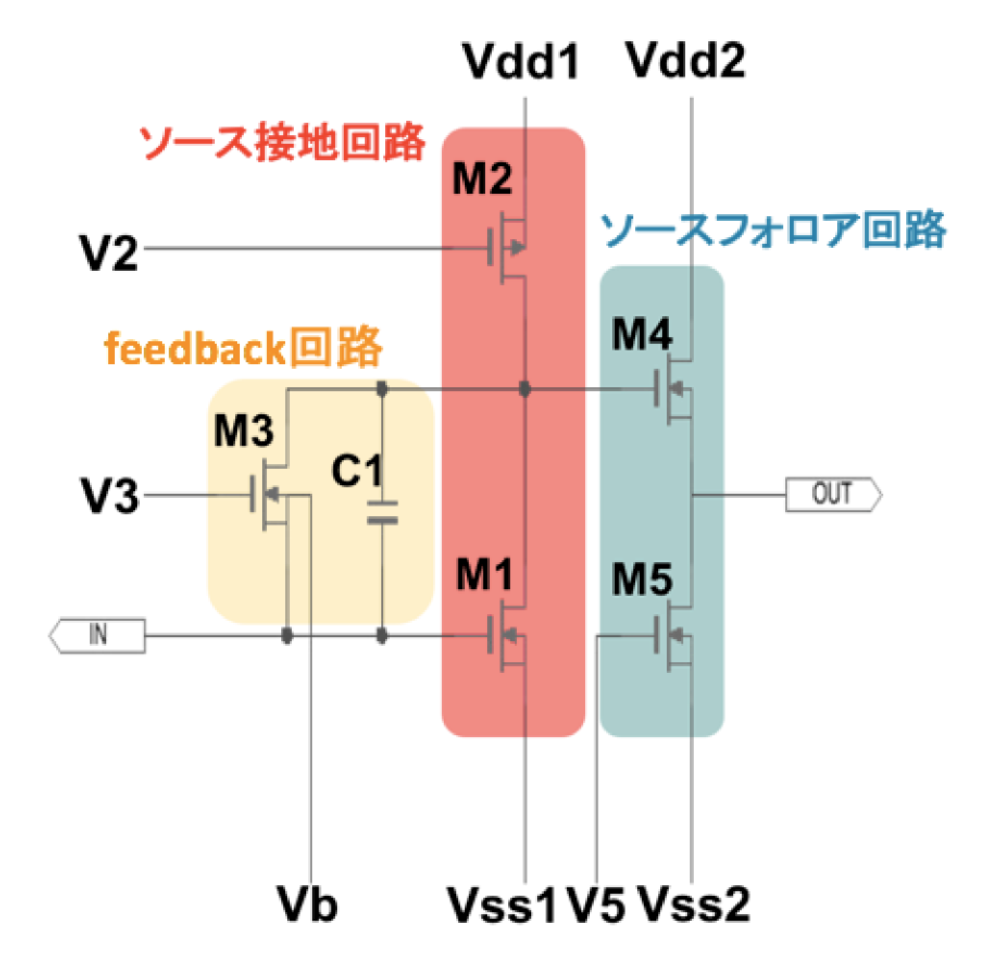
\includegraphics[width=10.0cm]{./Chapter/Chapter3/Picture/SOISTJ4_circuit.eps}
				\caption{極低温環境用SOI前置増幅器4号機(SOI-STJ4)}
				\label{fig:SOISTJ4_circuit}
			\end{center}
		\end{figure}
		\begin{table}[htb]
			\begin{center}
				\begin{tabular}{| c | l | c | c | c |} \hline
					Device ID & Device Type & Channel Width & Channel Length & Cap. \\ \hline \hline
					M1 & core lvt NMOS st2 & $40 \mathrm{\mu m}$ & $1 \mathrm{\mu m}$ & - \\ \hline
					M2 & core lvt PMOS st2 & $1 \mathrm{\mu m}$ & $10 \mathrm{\mu m}$ & - \\ \hline
					M3 & core lvt NMOS bt & $1.6 \mathrm{\mu m}$ & $10 \mathrm{\mu m}$ & - \\ \hline
					M4 & core lvt NMOS st2 & $70 \mathrm{\mu m}$ & $1 \mathrm{\mu m}$ & - \\ \hline
					M5 & core lvt NMOS st2 & $60 \mathrm{\mu m}$ & $1 \mathrm{\mu m}$ & - \\ \hline
					C1 & MIM capacitor & - & - & $100 \mathrm{fF}$ \\ \hline
				\end{tabular}
				\caption{SOI-STJ4に形成されているMOSFETの詳細}
				\label{tab:SOISTJ4_detail}
			\end{center}
		\end{table}
		前述したSOI-STJ3の問題点を解決するために、以下の変更を行った。
		\begin{description}
			\item[フィードバックコンデンサーを加えた]\mbox{}\\
				検出器側から見た入力インピーダンスを下げ、STJ信号を回路側へ伝送しやすくした。
			\item[STJ検出器とSOI-STJ4との間のコンデンサーの除去]\mbox{}\\
				前述の通り、このコンデンサーの静電容量はSTJ検出器の静電容量(数十〜数百pF)よりも十分大きくする必要がある。
				しかし、SOIプロセスで形成できるMIMキャパシタンスは$1.5 \mathrm{fF/{\mu m}^2}$であり、この大容量のキャパシタンスを形成するのは困難である。
				我々はSTJ検出器とSOI-STJ4との間のコンデンサーをSOIプロセスで作製せず、外付けのコンデンサーを用いることにする。
		\end{description}
		そして、SOI-STJ4について極低温環境下での性能評価を行った。
		\begin{figure}[htbp]
			\begin{center}
				\begin{tabular}{c}
					\begin{minipage}{0.5\hsize}
						\begin{center}
							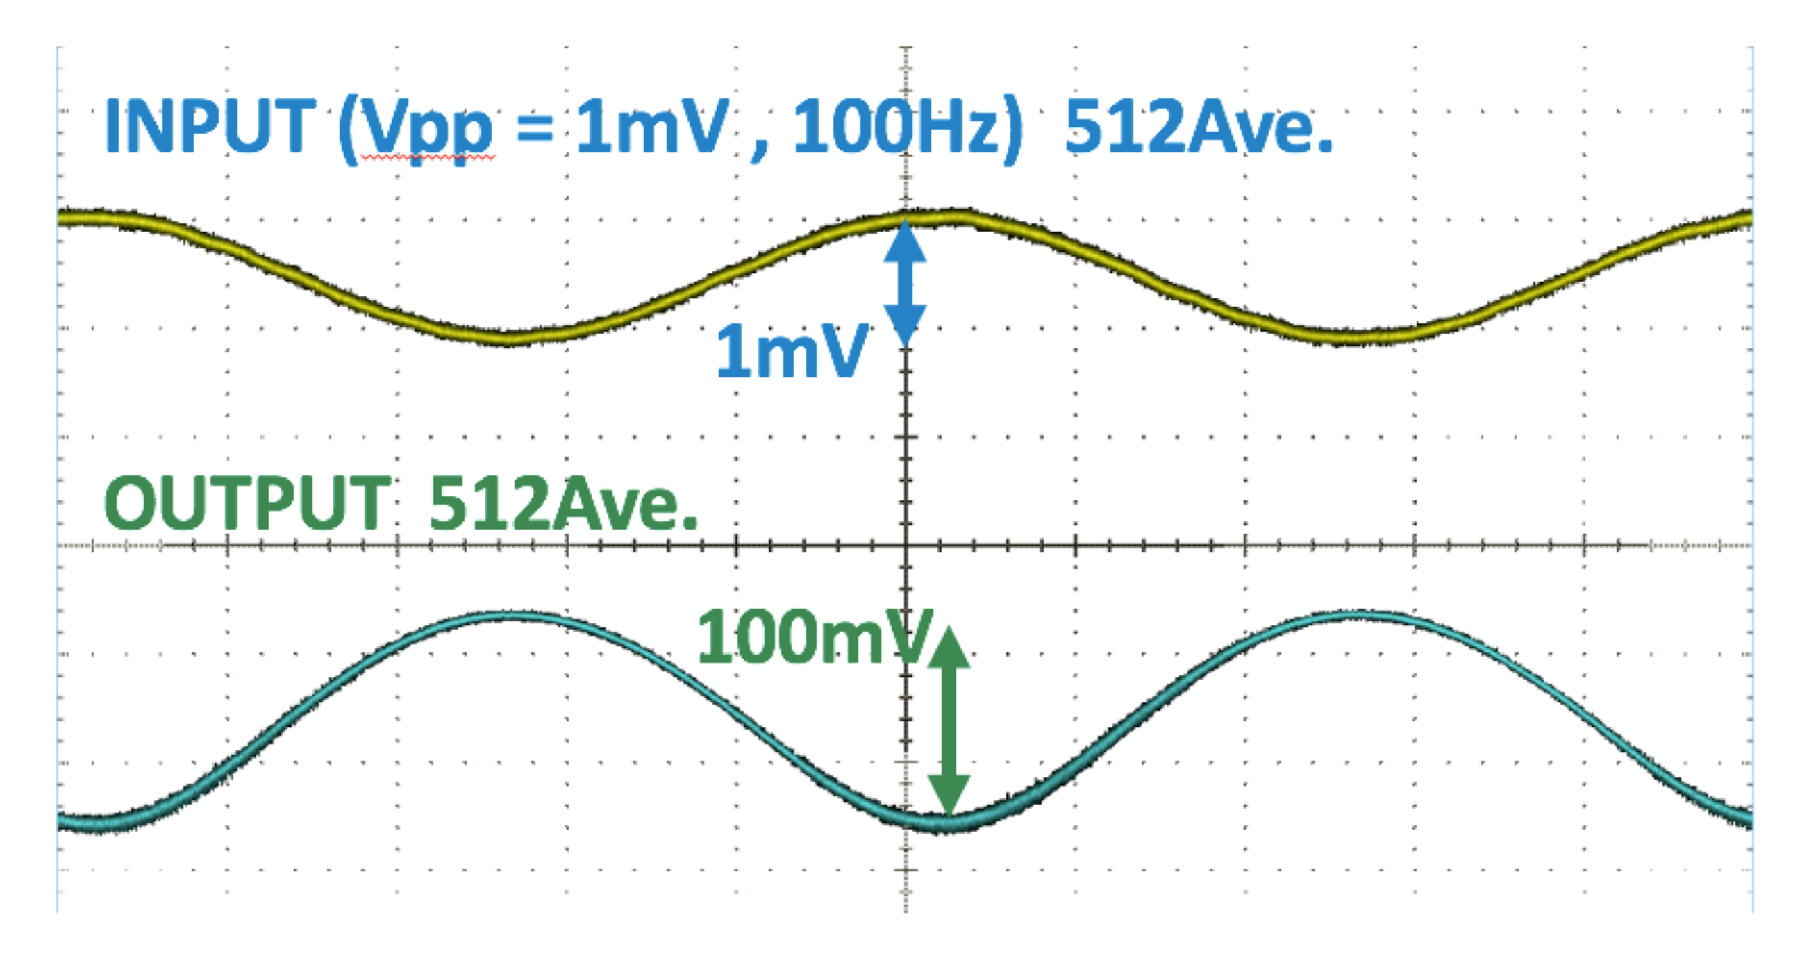
\includegraphics[clip, width=7.0cm]{./Chapter/Chapter3/Picture/SOISTJ4_InOut_100Hz.eps}
							\hspace{1.6cm} [a] 入出力電圧の関係(入力 : sin波(波高 : 1mV  周波数 : 100Hz))
						\end{center}
					\end{minipage}
					\begin{minipage}{0.5\hsize}
						\begin{center}
							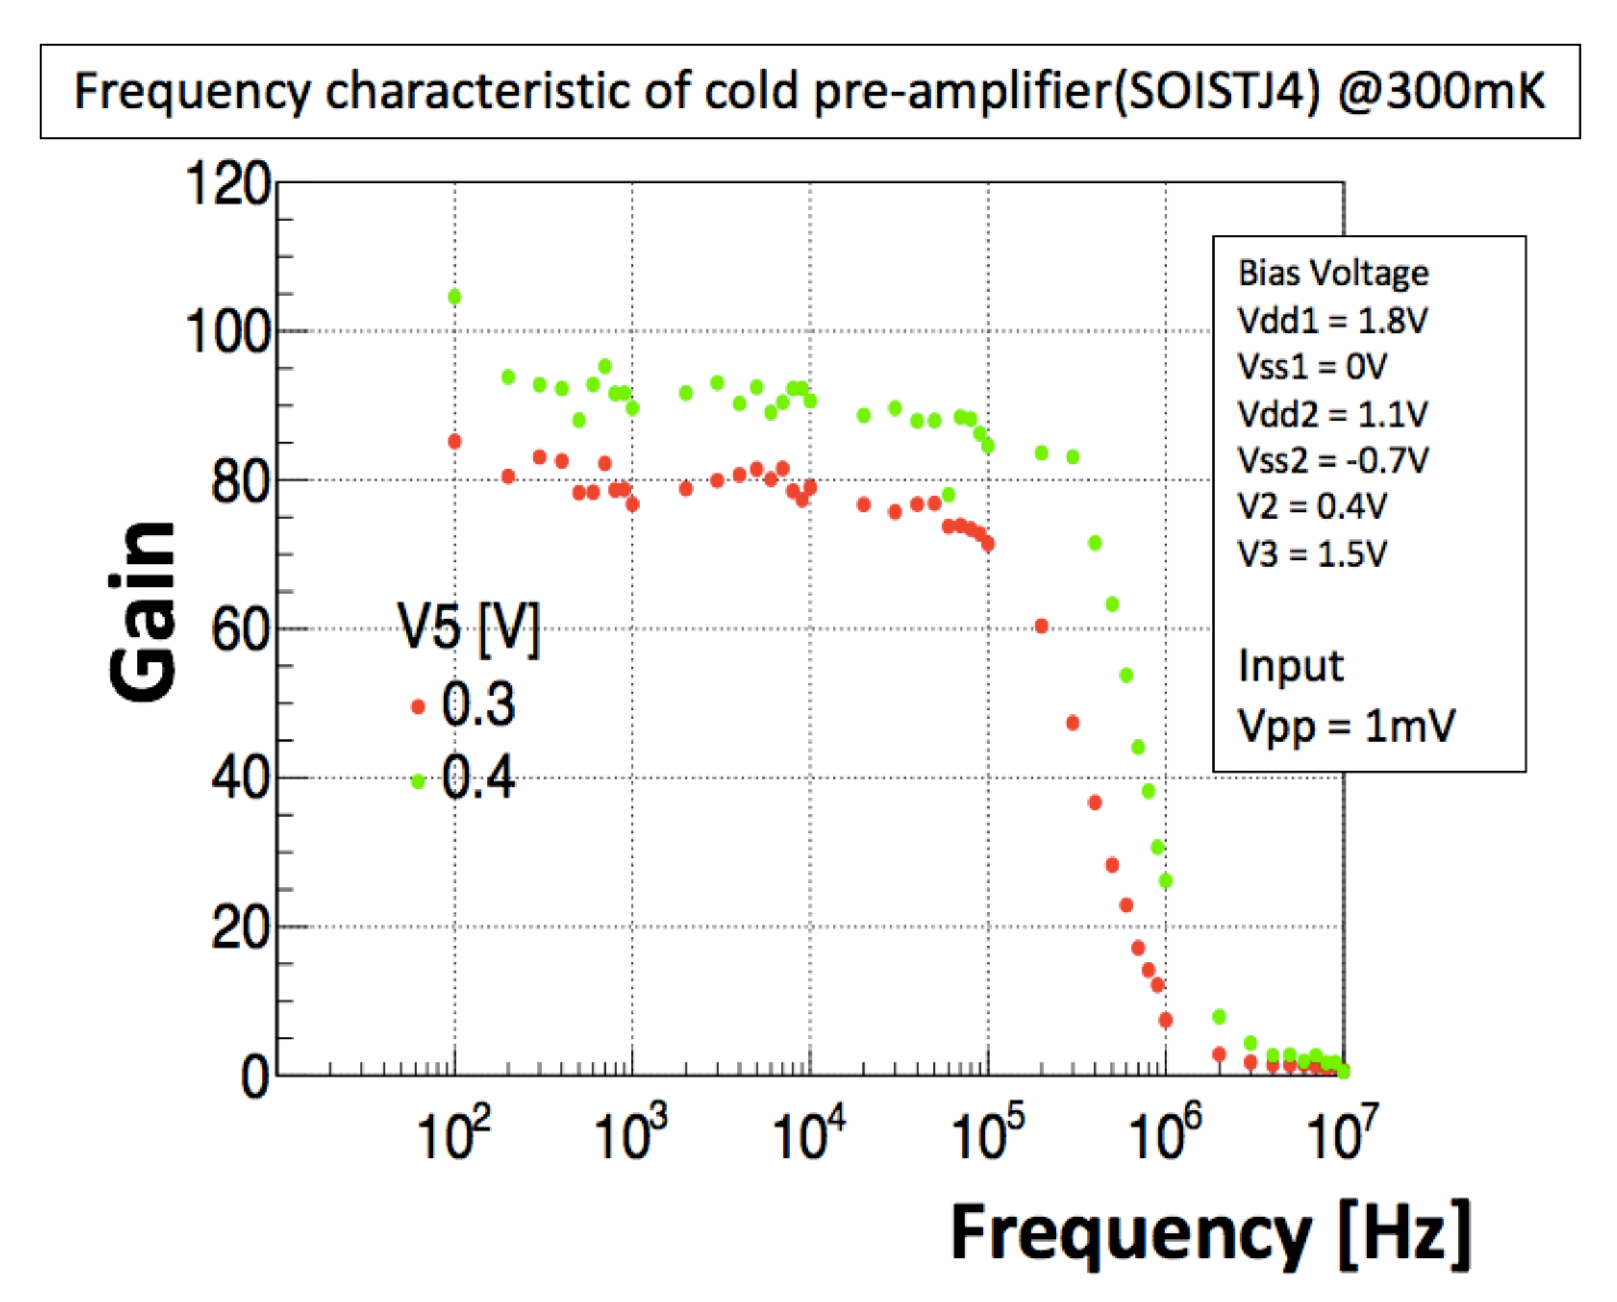
\includegraphics[clip, width=7.0cm]{./Chapter/Chapter3/Picture/SOISTJ4_frequency.eps}
							\hspace{1.6cm} [b] 極低温環境下での周波数特性
						\end{center}
					\end{minipage}
				\end{tabular}
				\caption{SOI-STJ4の極低温環境下での性能評価}
				\label{fig:SOISTJ4_chara}
			\end{center}
		\end{figure}
		\begin{figure}[htbp]
			\begin{center}
				\includegraphics[width=10.0cm]{./Chapter/Chapter3/Picture/SOISTJ4_InOut_1MHz.eps}
				\caption{SOI-STJ4にsin波(波高 : 1mV  周波数 : 1MHz)入力に対する出力}
				\label{fig:SOISTJ4_InOut_1MHz}
			\end{center}
		\end{figure}
		
		図\ref{fig:SOISTJ4_chara}にSOISTJ4の極低温環境下での性能評価を示した。
		図\ref{fig:SOISTJ4_chara}[a]はSOI-STJ4への入出力電圧を示している。黄線はSOI-STJ4への入力sin波(100Hz)であり、青線は出力電圧を示す。
		極低温環境下において、電圧利得は約100程度獲得できていることを確認できた。
		
		また図\ref{fig:SOISTJ4_chara}[b]は極低温環境下での周波数特性を示す。
		これによると、数百kHz程度までは安定して増幅できていることがわかる。
		またSTJ信号速度に対応する1MHzのsin波に対しては電圧利得30〜40を獲得できた。この時の入力と出力の関係を図\ref{fig:SOISTJ4_InOut_1MHz}に示す。
		
		以上より、極低温環境下でもSTJ検出器信号を十分増幅可能な回路が設計されていると考えられる。
		試験的にSTJ検出器に可視光レーザーを照射し、STJ検出器信号をSOI-STJ4に伝送させ増幅させる試験を行った。次章では、その試験結果について報告する。
		
		  %回折格子
	%\chapter{SOI増幅器を用いたSTJ信号増幅試験}
	\section{測定素子}
		\subsection{Nb/Al-STJ検出器}
			本測定では産業技術総合研究所(AIST)のCRAVITY製のNb/Al-STJ検出器を使用した。
			用いたNb/Al-STJ検出器の各層の厚みを表\ref{tab:NbAlSTJ_detail}に示す。
			\begin{table}[htb]
				\begin{center}
					\begin{tabular}{| l | c |} \hline
						\  & 厚さ[$\mathrm{nm}$] \\ \hline \hline
						上部ニオブ層 & 100 \\ \hline
						上部アルミニウム層 & 70 \\ \hline
						アルミナ$\mathrm{Al_{2}O_{3}}$ & 1 \\ \hline
						下部アルミニウム層 & 70 \\ \hline
						下部ニオブ層 & 100 \\ \hline
					\end{tabular}
					\caption{増幅試験に用いたSTJ検出器の厚さ}
					\label{tab:NbAlSTJ_detail}
				\end{center}
			\end{table}
			
			このSTJ検出器のマスクデザインを図\ref{fig:NbAlSTJ_mask}に示す。
			STJ信号増幅に用いたNb/Al-STJ検出器は図\ref{fig:NbAlSTJ_mask}の「Division3」に属する20$\mathrm{\mu m}$角のNb/Al-STJ検出器を用いた。
			
			\begin{figure}[htbp]
				\begin{center}
					\includegraphics[width=12.0cm]{./Chapter/Chapter4/Picture/NbAlSTJ_mask.eps}
					\caption{産総研CRAVITY製Nb/Al-STJ検出器\ マスクデザイン}
					\label{fig:NbAlSTJ_mask}
				\end{center}
			\end{figure}
		
			\clearpage
	\section{測定環境}
		\subsection{$\mathrm{^{3}He}$減圧冷凍機}
			\subsubsection{構造}
				我々はNb/Al-STJ検出器を300mK環境下で動作させるために、$\mathrm{^{3}He}$減圧冷凍機を用いて素子の冷却を行った。
				本研究に使用している$\mathrm{^{3}He}$減圧冷凍機は、Oxford Instruments社 HelioxAC-V $\mathrm{^{3}}$He Refrigeratorである。
				この$\mathrm{^{3}He}$減圧冷凍機は$\mathrm{^{3}He}$を減圧することによって冷却し、約300mK程度までの冷却を行うことができる。
								
				\begin{figure}[htbp]
					\begin{center}
						\begin{tabular}{c}
							%1
							\begin{minipage}{0.6\hsize}
								\begin{center}
									\includegraphics[clip, width=8cm]{./Chapter/Chapter4/Picture/He3_sorption_stage.eps}
									\hspace{1.6cm} [a]外観
								\end{center}
							\end{minipage}
							%2
							\begin{minipage}{0.4\hsize}
								\begin{center}
									\includegraphics[clip, width=4cm]{./Chapter/Chapter4/Picture/He3sorption_structure.eps}
									\hspace{1.6cm} [b]構造概念図
								\end{center}
							\end{minipage}
						\end{tabular}
						\caption{$\mathrm{^{3}He}$減圧冷凍機}
						\label{fig:He3sorption}
					\end{center}
				\end{figure}
				
				この冷凍機の冷却能力について、表\ref{tab:He3_sorption}に各ステージごとにまとめた。
				60Kステージ、3Kステージそれぞれには熱輻射シールドを設置している。
				またNb/Al-STJ検出器に外部から磁場が侵入しないようにパーマロイテープと呼ばれる磁場シールドも設置している。
				\begin{table}[htb]
					\begin{center}
						\begin{tabular}{| l | c | l |} \hline
							ステージ & 到達温度[K] & 冷却能力 \\ \hline
							60K & 60K & 25W\ @65K \\
							3K & 2.8K & 0.7W\ @4.2K \\
							最低温 & 0.3K & 100$\mathrm{\mu W}$\ @350mK \\ \hline
						\end{tabular}
						\caption{$\mathrm{^{3}He}$減圧冷凍機\ 各ステージの到達温度と冷却能力}
						\label{tab:He3_sorption}
					\end{center}
				\end{table}
				
				\clearpage
			
			\subsubsection{動作原理}
				\begin{figure}[htbp]
					\begin{center}
						\includegraphics[width=12.0cm]{./Chapter/Chapter4/Picture/He3sorption.eps}
						\caption{$\mathrm{^{3}He減圧冷凍機\ 動作概念図}$}
						\label{fig:He3sorption}
					\end{center}
				\end{figure}
				図\ref{fig:He3sorption}に$\mathrm{^{3}He}$減圧冷凍機の動作概念図を示した。
				まず、パルスチューブ冷凍機を用いて室温から3K程度まで冷却を行う。
				その後、図\ref{fig:He3sorption}のHeatSwitchを接続(close)することで、SorbとPTC 2nd Plateを熱伝導させることで3Kに冷却される。
				Sorbは冷却されることにより、Sorbには$\mathrm{^{3}He}$が吸着される。
				
				その後、HeatSwitchによる接続を解除(open)し、Sorbに付属しているHeaterで30K程度になるように熱を加える。
				すると、図\ref{fig:He3sorption}の左図のように、Sorbに吸着されていた$\mathrm{^{3}He}$が液化し、それが$\mathrm{^{3}He}$\ potに溜まる。
				そして、$\mathrm{^{3}He}$の液化後、SorbのHeaterの出力を止め、HeatSwitchによる接続(close)を行い、Sorbの冷却を再度行う。
				これにより、図\ref{fig:He3sorption}の右図のように、$\mathrm{^{3}He}$ potに溜まっている$\mathrm{^{3}He}$をSorbに吸着させることで、$\mathrm{^{3}He}$が減圧冷凍され、3Kから300mK程度までの冷凍がスタートする。
				\clearpage
	
	\section{SOI増幅器を用いたsin波増幅試験}
		我々は昨年度SOI-STJ4についての性能評価を行い、極低温環境下でSTJ検出器の信号を十分増幅可能な回路を設計できたと結論付けた。
		この結果を受け、我々は極低温環境下でSOI増幅器を用いたSTJ検出器信号の増幅試験を行った。
		
		そこで、まず我々はSTJ信号増幅の前にSOI-STJ4とNb/Al-STJを接続した回路であっても、SOI-STJ4が動作するかを確認するためにsin波増幅試験を行った。
		\subsection{SOI-STJ4のみのsin波増幅試験}
			\begin{figure}[htbp]
				\begin{center}
					\includegraphics[width=12.0cm]{./Chapter/Chapter4/Picture/SOISTJ4woSTJ_amp_sin.eps}
					\caption{SOI-STJ4のみを用いたsin波増幅試験\ 回路図}
					\label{fig:SOISTJ4woSTJ_amp_sin}
				\end{center}
			\end{figure}
			図\ref{fig:SOISTJ4woSTJ_amp_sin}にSOI-STJ4のみを用いたsin波増幅試験の回路図を示した。
			sin波入力にはFunction Generatorを用いており、周波数を走査させながら、出力波形を測定した。
			出力波形が飽和しないように、入力sin波の波高はpeak\ to\ peakで1mVとした。
			Function GeneratorとSOI-STJ4の入力端子との間には、常温環境下で4.7$\mathrm{\mu F}$の積層型セラミックコンデンサーを介し、AC的に接続をした。
			
			入出力波形はオシロスコープで読み取った。オシロスコープの設定は、
			\begin{itemize}
				\item 入力インピーダンス\ $1\mathrm{M \Omega}$
				\item AC結合
				\item 512回平均
			\end{itemize}
			である。
			入出力それぞれの波高(peak\ to\ peak)を取得し、利得Gainを式(\ref{eq:gain_definition})のように定義した。
			\begin{eqnarray}
				\mathrm{Gain} = \frac{V_{\mathrm{peak\ to\ peak}}(\mathrm{OUTPUT})}{V_{\mathrm{peak\ to\ peak}}(\mathrm{INPUT})}
				\label{eq:gain_definition}
			\end{eqnarray}
			
			\clearpage
			入力周波数が100Hzのとき、1MHzのとき、それぞれの入出力波形を図\ref{fig:SOISTJ4woSTJ_InOut_100Hz}と図\ref{fig:SOISTJ4woSTJ_InOut_1MHz}に示した。
			それぞれ黄線が入力波形、青線が出力波形を示す。
			
			まず$f_{\mathrm{input}=100\mathrm{Hz}}$のときの図\ref{fig:SOISTJ4woSTJ_InOut_100Hz}を見ると、入力に対し出力の位相が180度ずれて反転増幅していることがわかる。
			利得は約100程度である。
			対して、$f_{\mathrm{input}=1\mathrm{MHz}}$のときの図\ref{fig:SOISTJ4woSTJ_InOut_1MHz}を見ると、100Hzのときと比べると位相がずれて増幅されているのがわかる。
			そして利得は約30程度に下がっている。
			
			利得の周波数特性を示した図を図\ref{fig:SOISTJ4woSTJ_frequency}に示す。
			SOI-STJ4は入力周波数100kHz程度までは利得は落ちることなく増幅可能である。
			100kHzを超え始めると次第に利得は減少するが、冷凍機読み出し配線容量0.5nF、1MHz\ sin波に対し利得約30程度を獲得した。
			
			STJ検出器信号の速度が約$1\mathrm{\mu s}$であることからSTJ検出器信号を十分増幅できると示唆する結果を示せた。
			しかし、このときのSOI-STJ4の消費電力は$230\mathrm{\mu W}$で、最低温ステージ環境下での冷凍機の冷却能力を上回ってしまう。
			実際、SOI-STJ4の動作中の最低温ステージの温度は約300mKから約500から600mK程度まで上昇していた。
			この温度領域ではNb/Al-STJ検出器の熱雑音が落ちきらない。
			
			本実験では、SOI-STJ4を用いてのSTJ検出器信号を増幅させることが目的である。
			もしSOI-STJ4の動作によってNb/Al-STJ検出器が600mK程度までの温度上昇しても、Nb/Al-STJ検出器は超伝導検出器として動作する。
			したがって、本実験での200mK程度の温度上昇を問題としないこととする
			\footnote{我々はNb/Al-STJ検出器を熱起因雑音が落ちきる300mK環境下で動作させたいが、最低温ステージの冷却能力以下の消費電力で極低温前置増幅器を動作させるのは現状厳しい。そこで我々はSOI前置増幅器を3Kステージに設置し増幅させることを考えている。}。
			
			\begin{figure}[htbp]
				\begin{center}
					\includegraphics[width=12.0cm]{./Chapter/Chapter4/Picture/SOISTJ4woSTJ_InOut_100Hz.eps}
					\caption{SOI-STJ4のみを用いたsin波増幅試験\ 入出力波形($f_{\mathrm{input}}=100\mathrm{Hz}$)}
					\label{fig:SOISTJ4woSTJ_InOut_100Hz}
				\end{center}
			\end{figure}
			\begin{figure}[htbp]
				\begin{center}
					\includegraphics[width=12.0cm]{./Chapter/Chapter4/Picture/SOISTJ4woSTJ_InOut_1MHz.eps}
					\caption{SOI-STJ4のみを用いたsin波増幅試験\ 入出力波形($f_{\mathrm{input}}=100\mathrm{Hz}$)}
					\label{fig:SOISTJ4woSTJ_InOut_1MHz}
				\end{center}
			\end{figure}
			
			\begin{figure}[htbp]
				\begin{center}
					\includegraphics[width=12.0cm]{./Chapter/Chapter4/Picture/SOISTJ4woSTJ_frequency.eps}
					\caption{SOI-STJ4のみを用いたsin波増幅試験\ 利得の周波数依存性}
					\label{fig:SOISTJ4woSTJ_frequency}
				\end{center}
			\end{figure}
			\clearpage
			
		
		\subsection{Nb/Al-STJ検出器と組み合わせた回路でのSOI-STJ4を用いたsin波増幅試験}
			\begin{figure}[htbp]
				\begin{center}
					\includegraphics[width=12.0cm]{./Chapter/Chapter4/Picture/SOISTJ4wSTJ_amp_sin.eps}
					\caption{Nb/Al-STJ検出器と組み合わせた回路でのSOI-STJ4を用いたsin波増幅試験\ }
					\label{fig:SOISTJ4wSTJ_amp_sin}
				\end{center}
			\end{figure}
			300mK環境下におけるSOI-STJ4単体でのsin波増幅試験の結果、読み出し配線容量0.5nF、1MHz\ sin波に対して利得約30程度を観測した。
			次に、我々はNb/Al-STJ検出器と組み合わせた回路でSOI-STJ4のsin波増幅試験を行い、SOI-STJ4が前節と同様の性能を示すかを確かめる。
			図\ref{fig:SOISTJ4wSTJ_amp_sin}はNb/Al-STJ検出器と組み合わせた回路でのSOI-STJ4を用いたsin波増幅試験の回路図を示す。
			極低温環境下においてSTJ検出器の両端電圧を印加しなくてもジョセフソン電流が回路に流れてしまう。
			本測定ではジョセフソン電流を抑制するために磁場を印加しながら測定した。
			
			入力sin波、オシロスコープの設定は前節と同様の設定で行い、sin波の周波数を走査させながら入出力波形をオシロスコープで読み取った。
			
			入力sin波周波数$f_{\mathrm{input}}=100\mathrm{Hz}$のときの入出力波形を図\ref{fig:SOISTJ4wSTJ_InOut_100Hz}に示す。
			このときSOI-STJ4単体の場合と同様に利得97の反転増幅を観測した。
			そして、入力sin波周波数$f_{\mathrm{input}}=1\mathrm{MHz}$のときの入出力波形を図\ref{fig:SOISTJ4wSTJ_InOut_1MHz}に示す。
			この場合もSOI-STJ4単体の場合と同様に、入力波形と出力波形の位相はずれており、利得40程度の反転増幅を観測した。
			
			Nb/Al-STJ検出器を組み合わせた回路での利得の周波数特性を図\ref{fig:SOISTJ4wSTJ_frequency}に示す。
			SOI-STJ4単体の場合の利得の周波数依存性を示した図\ref{fig:SOISTJ4woSTJ_frequency}と同様の周波数特性を示していた。
			このことから、Nb/Al-STJ検出器と組み合わせてもSOI-STJ4は単体と同様の性能を示したことになる。
			
			\begin{figure}[htbp]
				\begin{center}
					\includegraphics[width=12.0cm]{./Chapter/Chapter4/Picture/SOISTJ4wSTJ_InOut_100Hz.eps}
					\caption{Nb/Al-STJ検出器と組み合わせた回路でのSOI-STJ4を用いたsin波増幅試験\ 入出力波形($f_{\mathrm{input}}=100\mathrm{Hz}$)}
					\label{fig:SOISTJ4wSTJ_InOut_100Hz}
				\end{center}
			\end{figure}
			\begin{figure}[htbp]
				\begin{center}
					\includegraphics[width=12.0cm]{./Chapter/Chapter4/Picture/SOISTJ4wSTJ_InOut_1MHz.eps}
					\caption{Nb/Al-STJ検出器と組み合わせた回路でのSOI-STJ4を用いたsin波増幅試験\ 入出力波形($f_{\mathrm{input}}=1\mathrm{MHz}$)}
					\label{fig:SOISTJ4wSTJ_InOut_1MHz}
				\end{center}
			\end{figure}
			\begin{figure}[htbp]
				\begin{center}
					\includegraphics[width=12.0cm]{./Chapter/Chapter4/Picture/SOISTJ4wSTJ_frequency.eps}
					\caption{Nb/Al-STJ検出器と組み合わせた回路でのSOI-STJ4を用いたsin波増幅試験\ 利得の周波数依存性}
					\label{fig:SOISTJ4wSTJ_frequency}
				\end{center}
			\end{figure}
			\clearpage
			
	\section{SOI増幅器とNb/Al-STJ検出器を組み合わせた回路での \newline Nb/Al-STJ検出器の電流電圧特性の測定}
		\begin{figure}[htbp]
			\begin{center}
				\includegraphics[width=8.0cm]{./Chapter/Chapter4/Picture/NbAlSTJwSOI_IV_circuit.eps}
				\caption{SOI-STJ4と組み合わせた回路でのNb/Al-STJ検出器の電流電圧特性\ 回路図}
				\label{fig:NbAlSTJwSOI_IV_circuit}
			\end{center}
		\end{figure}
		前節ではSOI-STJ4の性能評価について述べた。
		本節では、SOI-STJ4と組み合わせた回路上でNb/Al-STJ検出器の電流電圧特性について述べる。
		この測定の結果を用いて、SOI-STJ4を用いたNb/Al-STJ検出器信号増幅試験において、STJ検出器に流す定電流値を決める。
		
		本測定回路図を図\ref{fig:NbAlSTJwSOI_IV_circuit}に示す。
		Nb/Al-STJ検出器の電流電圧特性を基本的には4端子法で測定する。
		図\ref{fig:NbAlSTJwSOI_IV_circuit}中のCH1でSTJ検出器の両端電圧を読み出す。
		一方、図\ref{fig:NbAlSTJwSOI_IV_circuit}中のCH2では基準抵抗$\mathrm{R_{ref}}$間の両端の電圧を読み出すことで、Ohmの法則を用いてSTJ検出器に流れる電流値を計算する。
		
		注意すべきことは、SOI-STJ4とNb/Al-STJ検出器は$4.7\mathrm{\mu F}$のキャパシタンスでAC的に区切っている。
		しかし、SOI-STJ4が動作してしまうとSTJ検出器の電流電圧特性が変化して観測されてしまうので、SOI-STJ4の全ての端子をGNDに落として動作しないようにした。
		
		電流電圧特性の測定結果を図\ref{fig:NbAlSTJwSOI_IV_chara}に示す。
		本測定では0V付近でヒステリシス構造を持ち、図\ref{fig:STJ_IV}のような一般的なSTJ検出器の電流電圧特性と異なる構造を持つ。
		この原因として、我々が使う$\mathrm{^{3}He}$減圧冷凍機に搭載されている超電導コイルの不調でジョセフソン電流を抑制しきれなかったのが原因だと考えている。
		本節では超電導コイルが不調のままSOI-STJ4を用いたSTJ検出器信号増幅試験を行い、超電導コイル修理後にジョセフソン電流を十分抑制しきった状態で再試験を行う。
		\clearpage
		\begin{figure}[htbp]
			\begin{center}
				\includegraphics[width=10.0cm]{./Chapter/Chapter4/Picture/NbAlSTJwSOI_IV_chara.eps}
				\caption{SOI-STJ4と組み合わせた回路でのNb/Al-STJ検出器の電流電圧特性}
				\label{fig:NbAlSTJwSOI_IV_chara}
			\end{center}
		\end{figure}
		\begin{figure}[htbp]
			\begin{center}
				\includegraphics[width=10.0cm]{./Chapter/Chapter4/Picture/STJ_IV.eps}
				\caption{一般的なSTJ検出器の電流電圧特性}
				\label{fig:STJ_IV}
			\end{center}
		\end{figure}
		\clearpage
		
		次に、図\ref{fig:NbAlSTJwSOI_IV_circuit}の回路のまま、STJ検出器に可視光レーザーを照射したときに電流電圧特性がどのように変化するかを評価した。
		照射に用いた可視光レーザー(HAMAMATSU PICOSECOND LIGHT PULSER)の性能については表\ref{tab:lazer}に記した。
		\begin{table}[htb]
			\begin{center}
				\begin{tabular}{| l | l |} \hline
					レーザー & HAMAMATSU PICOSECOND LIGHT PULSER \\ \hline
					波長 & $465 \mathrm{nm}$ \\ \hline
					パルス幅 & $59$ps \\ \hline
					最大ピーク出力 & $149$mW \\ \hline \hline
					備考 & 1Hz〜100MHzの周波数で連続的に照射可能 \\ \hline
				\end{tabular}
				\caption{レーザーコントローラーの性能表}
				\label{tab:lazer}
			\end{center}
		\end{table}
		
		レーザー周波数を変化させたときのSTJ検出器の電流電圧特性を図\ref{fig:NbAlSTJwSOI_IV_chara_lazer}に示した。
		$-30 \mathrm{\mu A}$〜$30 \mathrm{nA}$でヒステリシス構造がある。
		本来この領域でSTJ検出器を動作させるが、このヒステリシス構造のため光応答試験においてこの領域は使えない。
		$30\mathrm{\mu A}$〜$50\mathrm{nA}$の領域において、レーザー照射「あり」の場合と「なし」の場合で0.1mV程度の応答が見える。
		SOI増幅器を用いたSTJ検出器信号増幅試験では、この領域でSTJ検出器を動作させる。
		\begin{figure}[htbp]
			\begin{center}
				\includegraphics[width=10.0cm]{./Chapter/Chapter4/Picture/NbAlSTJwSOI_IV_chara_lazer.eps}
				\caption{SOI-STJ4と組み合わせた回路でのNb/Al-STJ検出器の電流電圧特性\ レーザーを照射しながら測定した}
				\label{fig:NbAlSTJwSOI_IV_chara_lazer}
			\end{center}
		\end{figure}
		
		\clearpage
	\section{SOI増幅器を用いたSTJ検出器信号増幅試験}
		\begin{figure}[htbp]
			\begin{center}
				\includegraphics[width=10.0cm]{./Chapter/Chapter4/Picture/STJamp_circuit.eps}
				\caption{SOI-STJ4を用いたSTJ検出器信号増幅試験\ 回路図}
				\label{fig:STJamp_circuit}
			\end{center}
		\end{figure}
		本節ではSOI-STJ4を用いたNb/Al-STJ検出器信号増幅試験について述べる。
		増幅試験での回路図を図\ref{fig:STJamp_circuit}に示す。
		直流電源$\mathrm{V_{dc}}$と基準抵抗$10\mathrm{M\Omega}$をSTJ検出器に対して直列に接続する。
		Dynamic resistance領域でのSTJ検出器の抵抗は約$1\mathrm{M\Omega}$程度である。
		前節で述べたようにSTJ検出器には約$40\mathrm{nA}$程度の定電流を流しながら動作させたいので、直流電源$\mathrm{V_{dc}}$には0.4V程度印加する。
		もしSTJ検出器信号の波高が小さすぎる場合はこの直流電源を微調整する。
		レーザーは前節で述べた可視光レーザーを使用した。

		レーザー照射することでSTJ検出器の両端電圧が変化し、その信号をSOI-STJ4へ伝送することを考えている。
		SOI-STJ4の入力インピーダンスは約$200\mathrm{k\Omega}$程度であり、さらに1MHz帯域の信号に対して$4.7\mathrm{\mu F}$のキャパシタンスのインピーダンスは非常に小さい。
		このことから、STJ検出器信号はほぼSOI-STJ4側へ伝送される。
		
		本測定で我々は以下の2点について検証する。
		\begin{itemize}
			\item STJ検出器信号がSOI-STJ4へ伝送されるか
			\item 伝送されたSTJ検出器信号がSOI-STJ4を用いて増幅できるか
		\end{itemize}
		
		SOI-STJ4の入出力波形は差動増幅器とオシロスコープを用いて読み出された。
		オシロスコープの設定は、前節と同様
		\begin{itemize}
			\item 入力インピーダンス\ $1\mathrm{M \Omega}$
			\item AC結合
			\item 512回平均
		\end{itemize}
		である。
		
		\clearpage
		
		\subsection{測定結果}
			\begin{figure}[htbp]
				\begin{center}
					\includegraphics[width=10.0cm]{./Chapter/Chapter4/Picture/STJamp_lazer20k_raw.eps}
					\caption{SOI-STJ4を用いたSTJ検出器信号増幅試験(レーザー周波数$f_{\mathrm{lazer}=20\mathrm{kHz}}$\ 直流電源$V_{\mathrm{dc}}=0.43\mathrm{V}$)}
					\label{fig:STJamp_lazer20k_raw}
				\end{center}
			\end{figure}
		
			\begin{figure}[htbp]
				\begin{center}
					\includegraphics[width=10.0cm]{./Chapter/Chapter4/Picture/STJamp_lazer50k_raw.eps}
					\caption{SOI-STJ4を用いたSTJ検出器信号増幅試験(レーザー周波数$f_{\mathrm{lazer}=50\mathrm{kHz}}$\ 直流電源$V_{\mathrm{dc}}=0.43\mathrm{V}$)}
					\label{fig:STJamp_lazer50k_raw}
				\end{center}
			\end{figure}
			レーザー周波数を20kHzにした場合のSOI-STJ4への入力と出力の結果を図\ref{fig:STJamp_lazer20k_raw}に示した。
			同様に50kHzにした場合の結果を図\ref{fig:STJamp_lazer50k_raw}に示した。
			各図の黄線はSOI-STJ4への入力波形を示し、青線はSOI-STJ4の出力波形を示す。
			
			各図入力波形を見るとレーザーと同期して非常に小さなスパイクを観測できた。
			同様に出力波形を見るとレーザーと同期して正のピークを観測した。
			
			図\ref{fig:STJamp_lazer20k_raw_kakudai}と図\ref{fig:STJamp_lazer50k_raw_kakudai}入力波形の波高がかなり小さいので拡大した図である。
			各図の青線はSOI-STJ4への入力波形、橙線はSOI-STJ4の出力波形を示す。
			これらを見るとSOI-STJ4への入力波形は負のピークを持つことがわかる。
			各レーザー周波数ごとに入出力の波高を表\ref{tab:STJamp_vpp}に示した。
			\begin{table}[htb]
				\begin{center}
					\begin{tabular}{| l || l | l |} \hline
						レーザー周波数 & 入力波高 & 出力波高 \\ \hline \hline
						$20\mathrm{kHz}$ & $35 \mathrm{\mu V}$ & $1.4\mathrm{mV}$ \\ \hline
						$50\mathrm{kHz}$ & $33 \mathrm{\mu V}$ & $1.3\mathrm{mV}$ \\ \hline
					\end{tabular}
					\caption{レーザー周波数ごとの入出力波高}
					\label{tab:STJamp_vpp}
				\end{center}
			\end{table}
			
			SOI-STJ4への入力波形が、レーザーと同期して負にピークを持っている。
			レーザーを照射しながらSTJ検出器の電流電圧特性を測定した際、本測定で動作させる領域においてIVカーブが電圧が負の方向にシフトしていた。
			これらから、STJ検出器信号がSOI-STJ4に伝送されていたことがわかる。
			
			一方、SOI-STJ4の出力波形は入力波形とは逆に正のピークを持っている。
			SOI-STJ4のsin波増幅試験の結果の通り、SOI-STJ4回路には増幅段にソース接地増幅回路が入っているので入力に対して反転して増幅する。
			これらから、SOI-STJ4へ伝送されたSTJ検出器信号がSOI-STJ4で増幅されたことが実証された。
			
			FD-SOI-MOSFETを用いた前置増幅器が極低温環境下(300mK環境下)で信号読み出し可能であることから、我々が関わる素粒子実験分野に留まらず、低温読み出しを行う他分野への応用も期待される。
			
			今後としては、本実験でのSOI-STJ4に伝送された信号は何光子相当であったかなど、より定量的な解析を行う必要がある。
			\begin{figure}[htbp]
				\begin{center}
					\includegraphics[width=10.0cm]{./Chapter/Chapter4/Picture/STJamp_lazer20k_raw_kakudai.eps}
					\caption{SOI-STJ4を用いたSTJ検出器信号増幅試験(レーザー周波数$f_{\mathrm{lazer}=20\mathrm{kHz}}$\ 直流電源$V_{\mathrm{dc}}=0.43\mathrm{V}$)}
					\label{fig:STJamp_lazer20k_raw_kakudai}
				\end{center}
			\end{figure}
		
			\begin{figure}[htbp]
				\begin{center}
					\includegraphics[width=10.0cm]{./Chapter/Chapter4/Picture/STJamp_lazer50k_raw_kakudai.eps}
					\caption{SOI-STJ4を用いたSTJ検出器信号増幅試験(レーザー周波数$f_{\mathrm{lazer}=50\mathrm{kHz}}$\ 直流電源$V_{\mathrm{dc}}=0.43\mathrm{V}$)}
					\label{fig:STJamp_lazer50k_raw_kakudai}
				\end{center}
			\end{figure}
			
			
	
	
	  %SOI増幅器を用いたSTJ信号増幅試験
	%\chapter{極低温環境用SOI-FETの \newline SPICE回路シミュレーター構築}
	SPICE(Simulation Program with Integrated Circuit Emphasis)とは電子回路をシミュレーションするソフトウェアであり、1972年アメリカのカリフォルニア大学バークレイ校で開発された。
	以後、回路図エディタ、波形表示機能など様々な改良や機能拡張を加えたSPICEは回路シミュレータ業界では業界標準となっており、回路設計のために全世界で使われている。
	
	回路シミュレーションのメリットとしては、
	\begin{itemize}
		\item シミュレーションの際に測定系をわざわざ構築せずに済むのでコストを抑えられる
		\item 上記から、同時に時間短縮もでき、素子破壊の危険などを回避することもできる
		\item 実測不可の測定系でも、シミュレーター上の理想的な測定環境を考察することが可能
	\end{itemize}
	などが挙げられる。
	
	我々研究グループはSTJ検出器信号を増幅するための極低温環境用SOI前置増幅器の研究開発を行っており、回路設計の際には入念な回路シミュレーションが必要不可欠である。
	しかし、現在極低温環境用SPICE回路シミュレータは存在していないのが現状である。
	そのため、我々は極低温環境下でのSPICE回路シミュレーター構築を行った。
	
	シミュレーター構築の流れは、
	\begin{enumerate}
		\item 常温環境下で様々なサイズのFD-SOI-MOSFETについての電流電圧特性を測定
		\item 極低温環境下において、常温環境下と同様に電流電圧特性を測定
		\item 得られた電流電圧特性から、モデリングに必要なパラメーターを抽出
	\end{enumerate}
	である。我々筑波大はKEK\ 倉地氏のご助力を頂きながら電流電圧特性の測定の方を行い、JAXA\ 馬場氏にパラメーター抽出をしていただいた。
	我々が設計する増幅器はNb/Al-STJ検出器が動作する環境での動作を想定しており、よって300mK環境用のSPICE回路シミュレーターを構築する必要がある。
	我々の今までの測定において、3K環境下、300mK環境下でのFD-SOI-MOSFETの電流電圧特性に違いはほぼないことがわかっている。
	したがって、本構築では便宜上3K環境用SPICE回路シミュレーターを構築することとする。
	
	以後、我々が測定したサンプルの性能評価についての結果、並びに馬場氏に抽出していただいたパラメータを元に構築された極低温環境用SPICEパラメーターと実測の比較について述べる。
	\clearpage
	\section{測定サンプル}
		我々が測定したサンプルは、MOSFETの構造の違いからBody-Tie(BT)型とSource-Tie2(ST2)型の2種類に大別できる。
		このBT型とST2型についての構造上の違いについて以下述べる。
		\begin{description}
			\item[Body-Tie型]\mbox{}\\
				Body部の接続端子が外部まで配線されているMOSFETのこと。
			\item[Source-Tie2型]\mbox{}\\
				Source-Tie型とは、Body部がSourceと電気的に接続されている構造を持つ。
				BodyとSourceが電気的に接続されているため浮遊容量を抑えることができる。\\
				このSource-Tie型にはSource-Tie(ST)型とSource-Tie2(ST2)型に大別でき、これはBodyとSourceが電気的に接続される場所と面積が異なる。
		\end{description}
		各MOSFETのIDとサイズについての詳細を表\ref{tab:BT_detail}と表\ref{tab:ST_detail}に示す。
		\begin{table}[htb]
			\begin{center}
				\begin{tabular}{| c | l | c | c |} \hline
					Device ID & Device Type & Channel Length & Channel Width \\ \hline \hline
					B1 & core nvt NMOS bt & $0.2 \mathrm{\mu m}$ & $0.4 \mathrm{\mu m}$ \\ \hline
					B2 & core nvt NMOS bt & $0.2 \mathrm{\mu m}$ & $5 \mathrm{\mu m}$ \\ \hline
					B3 & core nvt NMOS bt & $10 \mathrm{\mu m}$ & $5 \mathrm{\mu m}$ \\ \hline
					B4 & core nvt NMOS bt & $10 \mathrm{\mu m}$ & $0.4 \mathrm{\mu m}$ \\ \hline \hline
					B5 & core nvt PMOS bt & $0.2 \mathrm{\mu m}$ & $0.5 \mathrm{\mu m}$ \\ \hline
					B6 & core nvt PMOS bt & $0.2 \mathrm{\mu m}$ & $5 \mathrm{\mu m}$ \\ \hline
					B7 & core nvt PMOS bt & $10 \mathrm{\mu m}$ & $5 \mathrm{\mu m}$ \\ \hline
					B8 & core nvt PMOS bt & $10 \mathrm{\mu m}$ & $0.63 \mathrm{\mu m}$ \\ \hline
				\end{tabular}
				\caption{測定したBody-Tie型FD-SOI-MOSFETの詳細}
				\label{tab:BT_detail}
			\end{center}
		\end{table}
		
		\begin{table}[htb]
			\begin{center}
				\begin{tabular}{| c | l | c | c |} \hline
					Device ID & Device Type & Channel Length & Channel Width \\ \hline \hline
					NS1 & core lvt NMOS st2 & $0.4 \mathrm{\mu m}$ & $1 \mathrm{\mu m}$ \\ \hline
					NS2 & core lvt NMOS st2 & $0.4 \mathrm{\mu m}$ & $2 \mathrm{\mu m}$ \\ \hline
					NS3 & core lvt NMOS st2 & $0.4 \mathrm{\mu m}$ & $10 \mathrm{\mu m}$ \\ \hline
					NS4 & core lvt NMOS st2 & $1 \mathrm{\mu m}$ & $10 \mathrm{\mu m}$ \\ \hline
					NS5 & core lvt NMOS st2 & $5 \mathrm{\mu m}$ & $10 \mathrm{\mu m}$ \\ \hline
					NS6 & core lvt NMOS st2 & $1 \mathrm{\mu m}$ & $1 \mathrm{\mu m}$ \\ \hline
					NS7 & core lvt NMOS st2 & $5 \mathrm{\mu m}$ & $1 \mathrm{\mu m}$ \\ \hline
					NS8 & core lvt NMOS st2 & $1 \mathrm{\mu m}$ & $2 \mathrm{\mu m}$ \\ \hline \hline
					PS1 & core lvt PMOS st2 & $0.4 \mathrm{\mu m}$ & $1 \mathrm{\mu m}$ \\ \hline
					PS2 & core lvt PMOS st2 & $0.4 \mathrm{\mu m}$ & $2 \mathrm{\mu m}$ \\ \hline
					PS3 & core lvt PMOS st2 & $0.4 \mathrm{\mu m}$ & $10 \mathrm{\mu m}$ \\ \hline
					PS4 & core lvt PMOS st2 & $1 \mathrm{\mu m}$ & $10 \mathrm{\mu m}$ \\ \hline
					PS5 & core lvt PMOS st2 & $5 \mathrm{\mu m}$ & $10 \mathrm{\mu m}$ \\ \hline
					PS6 & core lvt PMOS st2 & $1 \mathrm{\mu m}$ & $1 \mathrm{\mu m}$ \\ \hline
					PS7 & core lvt PMOS st2 & $5 \mathrm{\mu m}$ & $1 \mathrm{\mu m}$ \\ \hline
					PS8 & core lvt PMOS st2 & $1 \mathrm{\mu m}$ & $2 \mathrm{\mu m}$ \\ \hline
				\end{tabular}
				\caption{測定したSource-Tie型FD-SOI-MOSFETの詳細}
				\label{tab:ST_detail}
			\end{center}
		\end{table}
		\clearpage

	\section{電流電圧特性\ 測定環境}
		\subsection{測定系}
			\begin{figure}[htbp]
				\begin{center}
					\includegraphics[width=12.0cm]{./Chapter/Chapter5/Picture/IVmeasurement_circuit.eps}
					\caption{MOSFETの電流電圧特性の測定回路図(NMOSFETの場合)}
					\label{fig:IVmeasurement_circuit}
				\end{center}
			\end{figure}
			\begin{table}[htb]
				\begin{center}
					\begin{tabular}{| c | c | c |} \hline
						材質 & 配線抵抗$R_{refregerator}$ & 配線容量$C_{refregerator}$ \\ \hline \hline
						コンスタンタン & 約$70 \mathrm{\Omega}$程度 & 約$0.5 \mathrm{nF}$程度 \\ \hline
					\end{tabular}
					\caption{$\mathrm{^{3}He}$減圧冷凍機 読み出し配線の詳細}
					\label{tab:refregerator_wire}
				\end{center}
			\end{table}
			MOSFETの電流電圧特性の測定回路図を図\ref{fig:IVmeasurement_circuit}に示す。
			MOSFETを冷凍機内に設置し、長い冷凍機配線を経て室温に読み出し線を出す。この読み出し配線の詳細についてを表\ref{tab:refregerator_wire}にまとめた。\\
			電流電圧特性の測定にはソースメータ(KEITHLEY 2401)を用いた。
			PC上で各端子に印加する電圧を設定し、GPIBを介して各ソースメーターがMOSFETの各端子に電圧を印加し、そのときの電流値を測定するように命令を送る。
			そのときの測定値をPC上に保存するようにした。
		\subsection{測定項目}
			各デバイスごとに測定した電流電圧特性は、
			\begin{itemize}
				\item ドレイン電流のゲート電圧依存性($I_{ds}-V_{gs}$特性)
				\item ドレイン電流のドレイン電圧依存性($I_{ds}-V_{ds}$特性)
			\end{itemize}
			の2種類である。それぞれの依存性について常温環境下、3K環境下それぞれ測定した。\\
			以下2つのドレイン電流のバイアス電圧依存性の測定の際に印加した電圧について、MOSFETのタイプごとに表に示した。
			\begin{table}[htb]
				\begin{center}
					\begin{tabular}{| l c |} \hline \hline
						{\bf $I_{ds}-V_{gs}$特性} & \ \\ \hline
						$V_{body}\ =\  0\ \mathrm{V}$ & \ \\
						$V_{source}\ =\ 0\ \mathrm{V}$ & \ \\
						$V_{d}\ =\ 0.05\ /\ 1.8\ \mathrm{V}$ & 2\ points \\
						$V_{g}\ =\ 0\ \mathrm{V}\ \mathrm{to}\ 2\ \mathrm{V}$\ \ Step\ $0.02\ \mathrm{V}$ & 101\ points \\ \hline \hline
						{\bf $I_{ds}-V_{ds}$特性} & \ \\ \hline
						$V_{body}\ =\  0\ \mathrm{V}$ & \ \\
						$V_{source}\ =\ 0\ \mathrm{V}$ & \ \\
						$V_{g}\ =\ 0\ /\ 0.4\ /\ 0.8\ /\ 1.2\ /\ 1.6\ /\ 2.0\ \mathrm{V}$ & 6\ points \\
						$V_{d}\ =\ 0\ \mathrm{V}\ \mathrm{to}\ 2\ \mathrm{V}$\ \ Step\ $0.1\ \mathrm{V}$ & 21\ points \\ \hline
					\end{tabular}
					\caption{MOSFET(Device Type : core nvt NMOS Body-Tie)の電流電圧特性測定\\各電圧のパラメータ}
					\label{tab:NBT_bias}
				\end{center}
			\end{table}

			\begin{table}[htb]
				\begin{center}
					\begin{tabular}{| l c |} \hline \hline
						{\bf $I_{ds}-V_{gs}$特性} & \ \\ \hline
						$V_{body}\ =\  1.8\ \mathrm{V}$ & \ \\
						$V_{source}\ =\ 1.8\ \mathrm{V}$ & \ \\
						$V_{d}\ =\ 1.75\ /\ 0\ \mathrm{V}$ & 2\ points \\
						$V_{g}\ =\ 1.8\ \mathrm{V}\ \mathrm{to}\ -0.2\ \mathrm{V}$\ \ Step\ $-0.02\ \mathrm{V}$ & 101\ points \\ \hline \hline
						{\bf $I_{ds}-V_{ds}$特性} & \ \\ \hline
						$V_{body}\ =\  1.8\ \mathrm{V}$ & \ \\
						$V_{source}\ =\ 1.8\ \mathrm{V}$ & \ \\
						$V_{g}\ =\ 1.8\ /\ 1.4\ /\ 1.0\ /\ 0.6\ /\ 0.2\ /\ -0.2\ \mathrm{V}$ & 6\ points \\
						$V_{d}\ =\ 1.8\ \mathrm{V}\ \mathrm{to}\ -0.2\ \mathrm{V}$\ \ Step\ $-0.1\ \mathrm{V}$ & 21\ points \\ \hline
					\end{tabular}
					\caption{MOSFET(Device Type : core nvt PMOS Body-Tie)の電流電圧特性測定\\各電圧のパラメータ}
					\label{tab:PBT_bias}
				\end{center}
			\end{table}
			
			\begin{table}[htb]
				\begin{center}
					\begin{tabular}{| l c |} \hline \hline
						{\bf $I_{ds}-V_{gs}$特性} & \ \\ \hline
						$V_{source}\ =\ 0\ \mathrm{V}$ & \ \\
						$V_{d}\ =\ 0.05\ /\ 1.8\ \mathrm{V}$ & 2\ points \\
						$V_{g}\ =\ 0\ \mathrm{V}\ \mathrm{to}\ 2\ \mathrm{V}$\ \ Step\ $0.02\ \mathrm{V}$ & 101\ points \\ \hline \hline
						{\bf $I_{ds}-V_{ds}$特性} & \ \\ \hline
						$V_{source}\ =\ 0\ \mathrm{V}$ & \ \\
						$V_{g}\ =\ 0\ /\ 0.4\ /\ 0.8\ /\ 1.2\ /\ 1.6\ /\ 2.0\ \mathrm{V}$ & 6\ points \\
						$V_{d}\ =\ 0\ \mathrm{V}\ \mathrm{to}\ 2\ \mathrm{V}$\ \ Step\ $0.1\ \mathrm{V}$ & 21\ points \\ \hline
					\end{tabular}
					\caption{MOSFET(Device Type : core lvt NMOS Source-Tie)の電流電圧特性測定\\各電圧のパラメータ}
					\label{tab:NST_bias}
				\end{center}
			\end{table}

			\begin{table}[htb]
				\begin{center}
					\begin{tabular}{| l c |} \hline \hline
						{\bf $I_{ds}-V_{gs}$特性} & \ \\ \hline
						$V_{source}\ =\ 1.8\ \mathrm{V}$ & \ \\
						$V_{d}\ =\ 1.75\ /\ 0\ \mathrm{V}$ & 2\ points \\
						$V_{g}\ =\ 1.8\ \mathrm{V}\ \mathrm{to}\ -0.2\ \mathrm{V}$\ \ Step\ $-0.02\ \mathrm{V}$ & 101\ points \\ \hline \hline
						{\bf $I_{ds}-V_{ds}$特性} & \ \\ \hline
						$V_{source}\ =\ 1.8\ \mathrm{V}$ & \ \\
						$V_{g}\ =\ 1.8\ /\ 1.4\ /\ 1.0\ /\ 0.6\ /\ 0.2\ /\ -0.2\ \mathrm{V}$ & 6\ points \\
						$V_{d}\ =\ 1.8\ \mathrm{V}\ \mathrm{to}\ -0.2\ \mathrm{V}$\ \ Step\ $-0.1\ \mathrm{V}$ & 21\ points \\ \hline
					\end{tabular}
					\caption{MOSFET(Device Type : core lvt PMOS Source-Tie)の電流電圧特性測定\\各電圧のパラメータ}
					\label{tab:PST_bias}
				\end{center}
			\end{table}
			\clearpage 

	\section{電流電圧特性\ 測定結果}
		まず常温環境下でMOSFETの電流電圧特性の測定を行った。
		MOSFETの各端子に印加する電圧のパラメータはDevice Typeごとに表\ref{tab:NBT_bias}〜表\ref{tab:PST_bias}に記した。
		本節では、FD-SOI-MOSFETの型ごとに測定結果を述べる。
		\subsection{Body Tie型}
			Body Tie型のMOSFETの電流電圧特性を図\ref{fig:BT_N_IdVg}と図\ref{fig:BT_N_IdVd}に示す。
			
			図\ref{fig:BT_N_IdVg}は$I_{ds}-V_{gs}$特性を示す。図\ref{fig:BT_N_IdVg}[a]は常温環境下、図\ref{fig:BT_N_IdVg}[b]は3K環境下での特性を示す。
			両者を比較すると、
			\begin{itemize}
				\item 低温になるほど閾電圧の上昇
				\item サブスレッショルド領域でのドレイン電流の急激な上昇
			\end{itemize}
			を確認できた。
			
			また、図\ref{fig:BT_N_IdVd}は$I_{ds}-V_{ds}$特性を示す。図\ref{fig:BT_N_IdVd}[a]は常温環境下、図\ref{fig:BT_N_IdVd}[b]は3K環境下での特性を示す。
			先程と同様に両者を比較すると、
			\begin{itemize}
				\item 低温になるほど、飽和電流値の上昇
				\item 3K環境下において、ドレイン電圧が低い領域においてドレイン電流の立ち上がりの鈍化
				\item 3K環境下において、ドレイン電圧が高い領域においてドレイン電流の急な上昇
			\end{itemize}
			を確認できた。

			%=====Ids-Vgs特性=====%
			\begin{figure}[htbp]
				\begin{center}
					\begin{tabular}{c}
						%1
						\begin{minipage}{0.5\hsize}
							\begin{center}
								\includegraphics[clip, width=6cm]{./Chapter/Appendix/Picture/NBT/B3/PTEG2_8_B3_IdVg_room.eps}
								\hspace{1.6cm} [a]常温環境下
							\end{center}
						\end{minipage}
						%2
						\begin{minipage}{0.5\hsize}
							\begin{center}
								\includegraphics[clip, width=6cm]{./Chapter/Appendix/Picture/NBT/B3/PTEG2_8_B3_IdVg_3K.eps}
								\hspace{1.6cm} [b]3K環境下
							\end{center}
						\end{minipage}
					\end{tabular}
					\caption{Body Tie型(NMOS)の$I_{ds}-V_{gs}$特性\ Device ID : B3($W/L = 0.4\mathrm{\mu m} / 0.2\mathrm{\mu m}$)}
					\label{fig:BT_N_IdVg}
				\end{center}
			\end{figure}
			%=====Ids-Vds特性=====%
			\begin{figure}[htbp]
				\begin{center}
					\begin{tabular}{c}
						%1
						\begin{minipage}{0.5\hsize}
							\begin{center}
								\includegraphics[clip, width=6cm]{./Chapter/Appendix/Picture/NBT/B3/PTEG2_8_B3_IdVd_room.eps}
								\hspace{1.6cm} [a]常温環境下
							\end{center}
						\end{minipage}
						%2
						\begin{minipage}{0.5\hsize}
							\begin{center}
								\includegraphics[clip, width=6cm]{./Chapter/Appendix/Picture/NBT/B3/PTEG2_8_B3_IdVd_3K.eps}
								\hspace{1.6cm} [b]3K環境下
							\end{center}
						\end{minipage}
					\end{tabular}
					\caption{Body Tie型(NMOS)の$I_{ds}-V_{ds}$特性\ Device ID : B3($W/L = 0.4\mathrm{\mu m} / 0.2\mathrm{\mu m}$)}
					\label{fig:BT_N_IdVd}
				\end{center}
			\end{figure}
			
			\clearpage
			
		\subsection{Source-Tie2型}
		ST2型の電流電圧測定結果を図\ref{fig:ST_N_IdVg}と図\ref{fig:ST_N_IdVd}に示す。
		BT型と構造の異なるMOSFETでも、同様の電流電圧特性が現れていることを確認できた。
		
		また、全サンプルに対して、BT型と同様の電流電圧特性が現れていることを確認した。
		各Device Typeごとの全電流電圧特性の測定結果については、付録A章に示した。
		
		以上の結果をもとに我々は極低温環境下でのMOSFETの振る舞いについて調べた。
		我々が極低温環境下で用いるFD-SOI-MOSFETはST2型なので、以降の解析ではST2型についての解析のみ触れることにする。
			%=====Ids-Vgs特性=====%
			\begin{figure}[htbp]
				\begin{center}
					\begin{tabular}{c}
						%1
						\begin{minipage}{0.5\hsize}
							\begin{center}
								\includegraphics[clip, width=6cm]{./Chapter/Appendix/Picture/NST/NS6/PTEG2_10_NS6_IdVg_rmsetFL.eps}
								\hspace{1.6cm} [a]常温環境下
							\end{center}
						\end{minipage}
						%2
						\begin{minipage}{0.5\hsize}
							\begin{center}
								\includegraphics[clip, width=6cm]{./Chapter/Appendix/Picture/NST/NS6/PTEG2_10_NS6_IdVg_3K.eps}
								\hspace{1.6cm} [b]3K環境下
							\end{center}
						\end{minipage}
					\end{tabular}
					\caption{Source Tie型(NMOS)の$I_{ds}-V_{gs}$特性\ Device ID : NS6($W/L = 1\mathrm{\mu m} / 1\mathrm{\mu m}$)}
					\label{fig:ST_N_IdVg}
				\end{center}
			\end{figure}
			%=====Ids-Vds特性=====%
			\begin{figure}[htbp]
				\begin{center}
					\begin{tabular}{c}
						%1
						\begin{minipage}{0.5\hsize}
							\begin{center}
								\includegraphics[clip, width=6cm]{./Chapter/Appendix/Picture/NST/NS6/PTEG2_10_NS6_IdVd_rmsetFL.eps}
								\hspace{1.6cm} [a]常温環境下
							\end{center}
						\end{minipage}
						%2
						\begin{minipage}{0.5\hsize}
							\begin{center}
								\includegraphics[clip, width=6cm]{./Chapter/Appendix/Picture/NST/NS6/PTEG2_10_NS6_IdVd_3K.eps}
								\hspace{1.6cm} [b]3K環境下
							\end{center}
						\end{minipage}
					\end{tabular}
					\caption{Source Tie型(NMOS)の$I_{ds}-V_{ds}$特性\ Device ID : NS6($W/L = 1\mathrm{\mu m} / 1\mathrm{\mu m}$)}
					\label{fig:ST_N_IdVd}
				\end{center}
			\end{figure}

		
	\section{解析}
		\subsection{閾値電圧の温度依存性}
			ゲート界面の電位が高くなると、ゲート直下のボディ部の半導体の型が反転する。
			それに伴いドレイン電流が流れ始め、トランジスタとしては「オン」の状態になる。
			
			しかし、実際にはゲート電圧が高くなるに従ってMOSFETは徐々にオンの状態になるので、閾値電圧を明確に定義するのは非常に困難である。
			そこで我々はゲート電圧が閾値電圧になるときのドレイン電流を式(\ref{eq:Vth_definition})のように定義した。
			\begin{eqnarray}
				I_{ds} = 0.1[\mathrm{\mu A}] \times \frac{W}{L}
				\label{eq:Vth_definition}
			\end{eqnarray}
			
			この式(\ref{eq:Vth_definition})に従って、常温環境下と極低温環境下において閾値電圧の変動を検証した。
			検証した結果の各サンプルごとの閾値電圧を表\ref{tab:Vth_temp}にまとめた。
			どのサンプルも閾値電圧は室温時と比較して、3K時の閾値電圧の方が約0.2V程度高くなることがわかる。
			例として、図\ref{fig:ST_N_IdVg_Vth}に$I_{ds}-V_{gs}$特性を常温環境下と3K環境下で比較したサンプルを例として示す。
			%=====
			\begin{table}[htb]
			\centering
				\begin{tabular}{|c|cc|c|cc|cc|}
					\hline
					\multirow{3}{*}{ID} & \multirow{3}{*}{L[$\mathrm{\mu m}$]} & \multirow{3}{*}{W[$\mathrm{\mu m}$]} & \multirow{3}{*}{$I_{ds}(V_{gs}=V_{th})$A} & \multicolumn{2}{c|}{Room} & \multicolumn{2}{c|}{3K} \\ \cline{5-8} 
					 &  &  &  & \multicolumn{1}{c|}{$V_{ds} = 0.05V$} & $V_{ds} = 1.80V$ & \multicolumn{1}{c|}{$V_{ds} = 0.05$V} & $V_{ds} = 1.80$V \\
					 &  &  &  & \multicolumn{1}{c|}{$V_{th}$} & $V_{th}$ & \multicolumn{1}{c|}{$V_{th}$} & $V_{th}$ \\ \hline
					NS1 & 0.4 & 1 & $4 \times 10^{-8}$ & 0.64 & 0.59 & 0.97 & 0.77 \\
					NS2 & 0.4 & 2 & $2 \times 10^{-8}$ & 0.58 & 0.53 & 0.91 & 0.61 \\
					NS3 & 0.4 & 10 & $4 \times 10^{-9}$ & 0.59 & 0.55 & 0.95 & 0.63 \\
					NS4 & 1 & 10 & $1 \times 10^{-8}$ & 0.61 & 0.59 & 0.85 & 0.63 \\
					NS5 & 5 & 10 & $5 \times 10^{-8}$ & 0.61 & 0.61 & 0.81 & 0.69 \\
					NS6 & 1 & 1 & $1 \times 10^{-7}$ & 0.56 & 0.53 & 0.89 & 0.69 \\
					NS7 & 5 & 1 & $5 \times 10^{-7}$ & 0.60 & 0.57 & 0.93 & 0.79 \\
					NS8 & 1 & 2 & $5 \times 10^{-8}$ & 0.59 & 0.51 & 0.87 & 0.69 \\ \hline
				\end{tabular}
				\caption{各サイズごとの閾値電圧$V_{th}$の温度依存性(NMOS Source Tie2型)}
				\label{tab:Vth_temp}
			\end{table}
			\clearpage
			
			\begin{figure}[htbp]
				\begin{center}
					\begin{tabular}{c}
						%1
						\begin{minipage}{0.5\hsize}
							\begin{center}
								\includegraphics[clip, width=6.5cm]{./Chapter/Appendix/Picture/NST/NS6/PTEG10_NS6_IdVg_0.05_.log_.eps}
								\hspace{1.6cm} [a]ドレイン電圧$V_{ds}=0.05\mathrm{V}$
							\end{center}
						\end{minipage}
						%2
						\begin{minipage}{0.5\hsize}
							\begin{center}
								\includegraphics[clip, width=6.5cm]{./Chapter/Appendix/Picture/NST/NS6/PTEG10_NS6_IdVg_1.80_.log_.eps}
								\hspace{1.6cm} [b]ドレイン電圧$V_{ds}=1.80\mathrm{V}$
							\end{center}
						\end{minipage}
					\end{tabular}
					\caption{Source Tie型(NMOS)の$I_{ds}-V_{gs}$特性(縦軸 : 対数表示)\ Device ID : NS6($W/L = 1\mathrm{\mu m} / 1\mathrm{\mu m}$)}
					\label{fig:ST_N_IdVg_Vth}
				\end{center}
			\end{figure}
			
			\begin{figure}[htbp]
				\begin{center}
					\begin{tabular}{c}
						%1
						\begin{minipage}{0.5\hsize}
							\begin{center}
								\includegraphics[clip, width=6.5cm]{./Chapter/Appendix/Picture/NST/NS6/PTEG10_NS6_IdVg_0.05_.linear_.eps}
								\hspace{1.6cm} [a]ドレイン電圧$V_{ds}=0.05\mathrm{V}$
							\end{center}
						\end{minipage}
						%2
						\begin{minipage}{0.5\hsize}
							\begin{center}
								\includegraphics[clip, width=6.5cm]{./Chapter/Appendix/Picture/NST/NS6/PTEG10_NS6_IdVg_1.80_.linear_.eps}
								\hspace{1.6cm} [b]ドレイン電圧$V_{ds}=1.80\mathrm{V}$
							\end{center}
						\end{minipage}
					\end{tabular}
					\caption{Source Tie型(NMOS)の$I_{ds}-V_{gs}$特性(縦軸 : 線形表示)\ Device ID : NS6($W/L = 1\mathrm{\mu m} / 1\mathrm{\mu m}$)}
					\label{fig:ST_N_IdVg_Vth}
				\end{center}
			\end{figure}
			\clearpage

		\subsection{飽和電流値の温度依存性}
			飽和領域での飽和電流値はチャネル長変調効果を無視すると、式(\ref{eq:Ids_saturate})のように書くことができる。
			\begin{eqnarray}
				I_{ds} = \frac{1}{2} \mu(T) C_{OX} \frac{W}{L} {(V_{gs} - V_{th})}^2
				\label{eq:Ids_saturate}
			\end{eqnarray}
			ゲートキャパシタンス$C_{OX}$、MOSFETのサイズ$\frac{W}{L}$の温度変化を無視すると、ドレイン電流$I_{ds}$は、
			\begin{eqnarray}
				I_{ds} \propto \mu(T)
				\label{eq:Ids_saturate_2}
			\end{eqnarray}
			となる。移動度$\mu$は式(\ref{eq:Ids_saturate})では唯一温度に依存する項であり、ドレイン電流とは比例関係にある。
			一般的に極低温環境下においてキャリア移動度は、常温環境下と比べて大きくなる。したがって、極低温環境下での飽和電流値の方がドレイン電流は大きくなると予想できる。
			
			$V_{gs} = V_{ds} = 2V$でのドレイン電流値を飽和電流値として、常温環境下と3K環境下で比較した。
			比較した結果を表\ref{tab:Ids_saturate_temp}に示す。
			%=====表 飽和電流値の温度依存性=====%
			\begin{table}[htb]
				\centering
				\begin{tabular}{|c|cc|c|c|c|}
					\hline
					\multirow{2}{*}{ID} & \multirow{2}{*}{L[$\mathrm{\mu m}$]} & \multirow{2}{*}{W[$\mathrm{\mu m}$]} & Room & 3K & \multirow{2}{*}{Ratio($I_{ds}(3K)/I_{ds}(Room)$)} \\
					 &  &  & $I_{ds}(\mathrm{saturate})$[A] & $I_{ds}(\mathrm{saturate})$[A] &  \\ \hline
					NS1 & 0.4 & 1 & $2.05 \times 10^{-4}$ & $2.57 \times10^{-4}$ & 1.3 \\
					NS2 & 0.4 & 2 & $4.21 \times 10^{-4}$ & $5.47 \times 10^{-4}$ & 1.3 \\
					NS3 & 0.4 & 10 & $1.61 \times 10^{-3}$ & $2.06 \times 10^{-3}$ & 1.3 \\
					NS4 & 1 & 10 & $9.39 \times 10^{-4}$ & $1.41 \times 10^{-3}$ & 1.5 \\
					NS5 & 5 & 10 & $2.72 \times 10^{-4}$ & $6.01 \times 10^{-4}$ & 2.2 \\
					NS6 & 1 & 1 & $1.32 \times 10^{-4}$ & $1.89 \times 10^{-4}$ & 1.4 \\
					NS7 & 5 & 1 & $3.09 \times 10^{-5}$ & $5.97 \times 10^{-5}$ & 1.9 \\
					NS8 & 1 & 2 & $2.28 \times 10^{-4}$ & $3.46 \times 10^{-4}$ & 1.5 \\ \hline
				\end{tabular}
				\caption{各サイズごとの飽和電流値$I_{ds}(\mathrm{saturate})$の温度依存性(NMOS Source Tie2型)}
				\label{tab:Ids_saturate_temp}
			\end{table}
			%================================%
			
			表\ref{tab:Ids_saturate_temp}から、ドレイン電流の比は1.3以上2.2以下でバラついている。
			MOSFETのサイズ($W \times L$)が大きければ大きいほど、その比が大きくなる傾向にあるのが表からわかる。
			各MOSFETの電流電圧特性を見ると、MOSFETのサイズが大きければ大きいほど、Kink効果の影響が顕著に見えているのがわかる。
			この理由から、サイズが大きければ、その分飽和電流値の比が大きくなる。
			
			また、式(\ref{eq:Ids_saturate_2})から、常温と極低温環境下でのドレイン電流の比は、そのままキャリア移動度の比に相当する。
			したがって、もし2次効果など諸々を無視した理想的な飽和電流を仮定すると、キャリア移動度は極低温環境下では約1.5倍程度上昇することがわかる。
			しかし、実際には特にチャネル長変調効果は無視できないので、以後キャリア移動度比についての検証について議論することにする。
			\clearpage
		\subsection{常温・極低温環境下でのキャリア移動度の比較}
			極低温環境下でのキャリア移動度は常温環境下でのキャリア移動度に比べて大きくなることが前節までの解析で明らかになった。
			では、実際にどれだけ大きくなるのかを定量的に考察することにする。
			
			まず、線形領域、飽和領域でMOSFETを動作させたときのドレイン電流の式は以下のように書くことができる。
			\begin{eqnarray}
				I_{ds}(\mathrm{linear}) & = & \mu C_{OX} \frac{W}{L} \{ (V_{gs} - V_{th})V_{ds} - \frac{1}{2}{V_{ds}}^2 \} \\
				I_{ds}(\mathrm{saturate}) & = & \mu C_{OX} \frac{W}{L} {(V_{gs} - V_{th})}^2
			\end{eqnarray}
			上式では、チャネル長変調効果を無視した。これらの式を変形すると、式(\ref{eq:mu_linear})、式(\ref{eq:mu_saturate})のようになる。
			\begin{eqnarray}
				\mu C_{OX} \frac{W}{L} & = & -\frac{{\partial}^2 I_{ds}}{\partial {V_{gs}}^2} \ \mathrm{(線形領域)}
				\label{eq:mu_linear} \\
				\mu C_{OX} \frac{W}{L} & = & 2 {(\frac{\partial \sqrt{I_{ds}}}{\partial V_{gs}})}^2 \ \mathrm{(飽和領域)}
				\label{eq:mu_saturate} \\
			\end{eqnarray}
			各式の左辺に着目すると、温度に依存する項はキャリア移動度$\mu$のみである。
			したがって、常温環境下と極低温環境下のそれぞれで右辺の値を計算し比をとることで、常温環境下と極低温環境下のキャリア移動度の比を求めたことになる。
			
			しかし、極低温環境下でドレイン電圧$V_{ds}$が低い領域において、MOSFETの電流電圧特性モデルとは異なるドレイン抵抗の異常な上昇が見られている。
			この効果を回避した領域での解析を行うため、本解析では飽和領域でのみの解析、検証を行った。
			
			\begin{figure}[htbp]
				\begin{center}
					\begin{tabular}{c}
						%1
						\begin{minipage}{0.5\hsize}
							\begin{center}
								\includegraphics[clip, width=6.5cm]{./Chapter/Appendix/Picture/NST/mu_analysis/mu_NS6.eps}
								\hspace{1.6cm} [a]NS6($W/L = 1\mathrm{\mu m}/1\mathrm{\mu m}$)
							\end{center}
						\end{minipage}
						%2
						\begin{minipage}{0.5\hsize}
							\begin{center}
								\includegraphics[clip, width=6.5cm]{./Chapter/Appendix/Picture/NST/mu_analysis/mu_NS5.eps}
								\hspace{1.6cm} [b]NS5($W/L = 10\mathrm{\mu m}/5\mathrm{\mu m}$)
							\end{center}
						\end{minipage}
					\end{tabular}
					\caption{飽和領域におけるキャリア移動度温度依存性の検証 \newline 
						(縦軸:$\mu C_{OX} \frac{W}{L}$ 横軸 : ゲート電圧$V_{gs}$)  (赤線:常温環境 緑線:3K環境下)}
					\label{fig:mu_analysis}
				\end{center}
			\end{figure}
			
			図\ref{fig:mu_analysis}にその解析結果として、NMOS-ST2型のNS6($W/L = 1\mathrm{\mu m}/1\mathrm{\mu m}$)とNS5($W/L = 10\mathrm{\mu m}/5\mathrm{\mu m}$)の結果を例として示す。
			
			赤線が常温環境下、緑線が3K環境下での結果である。それぞれの結果を見比べると、常温環境下では大きなピークは一つしか見られないのに対し、3K環境下では2つの大きなピークがみえる。
			3K環境下のVgsが低い方の大きな鋭いピークの位置は、$I_{ds}-V_{gs}$特性でのドレイン電流が指数関数的に上昇するサブスレッショルド領域に相当する。
			電流電圧特性測定の結果のサブスレッショルド領域を見ると常温環境に比べ、3Kでは非常に立ち上がりが早い。
			本解析でのこの鋭いピークはこの影響が見れていると推測される。
			
			次に、3K環境下のプロットにおいてゲート電圧$V_{gs}$が高い領域でのピークの最大値$\mu(\mathrm{3K}) C_{OX} \frac{W}{L}$と、常温環境下での$\mu(\mathrm{3K}) C_{OX} \frac{W}{L}$の最大値の最大値を求める。
			そして、Wで規格化してLの長さが同じサンプル同士で移動度を比較する。比較した結果を図\ref{fig:mu_analysis_size}に示す。
			全てのサンプルは、常温環境下の$\mu C_{OX} \frac{1}{L}$値に比べて3K環境下での$\mu C_{OX} \frac{1}{L}$値の方が大きいことがわかる。
			
			前述の通り、もしゲートキャパシタンス$C_{OX}$やMOSFETのサイズが温度依存しないとすると、$\mu C_{OX} \frac{1}{L}$に温度依存する項はキャリア移動度$\mu$のみであり、$\mu C_{OX} \frac{1}{L}$値の比が室温環境下でのキャリア移動度と極低温環境下でのキャリア移動度の比に相当するはずである。
			したがって、この仮定が正しければチャネル長Lが同じサンプル同士で$\mu C_{OX} \frac{1}{L}$値を比べた場合、全てのサンプルに対して$\mu C_{OX} \frac{1}{L}$比は同じはずである。
			しかし、実際はサンプルごとにその比はかなり異なっており、結果としてキャリア移動度比の検証を行うことができなかった。
			
			まとめると、前節の飽和電流値の温度依存性の結果、本節の解析結果はキャリア移動度は上昇していることを示唆する結果であるが、極低温環境下におけるキャリア移動度を定量的に求めることはできなかった。
			
			\begin{figure}[htbp]
				\begin{center}
					\includegraphics[clip,width=15.0cm]{./Chapter/Appendix/Picture/NST/mu_analysis/mu_analysis_size.eps}
					\caption{各サイズごとの$\mu C_{OX} \frac{1}{L}$値(縦軸:$\mu C_{OX} \frac{1}{L}$ 横:MOSFETのサイズ)}
					\label{fig:mu_analysis_size}
				\end{center}
			\end{figure}
			\clearpage
			
	\section{シミュレーション構築}
		\subsection{シミュレーション}
			我々研究グループが測定したFD-SOI-MOSFETの電流電圧特性の測定結果をもとにJAXA\ 馬場氏にモデリングに必要なパラメータ抽出をしていただいた。
			抽出していただいたパラメータを筑波大PC環境のもとhspice回路シミュレーター、及びngspice回路シミュレーターにて適応させ、シミュレーションを行った。
			
			極低温環境下において、ドレイン電圧$V_{ds}$が低い領域においてドレイン抵抗が異常に大きくなる現象が確認されている。
			この極低温環境特有の特性を現在のMOSFETの電流電圧特性モデルで表現することは不可なので、パラメータ抽出のためのフィッティング領域は飽和領域のみに限定する。
			
			パラメータ抽出を行うトランジスタを表\ref{tab:extract_transistor}にまとめた。
			
			抽出したパラメータをもとにhspiceとngspiceを用いてMOSFETの電流電圧特性のシミュレーションを行い、実測と比較した。
			次節では、その結果について述べる。
			\begin{table}[htb]
				\begin{center}
					\begin{tabular}{| c | c | c |} \hline
						Device Type & Channel Length L & Channel Width \\ \hline \hline
						Body Tie(Nch/Pch) & 0.2$\mathrm{\mu m}$ & 5.0$\mathrm{\mu m}$ \\ \hline
						Source Tie2(Nch/Pch) & 0.4$\mathrm{\mu m}$ & 10$\mathrm{\mu m}$ \\
						\ & 1.0$\mathrm{\mu m}$ & 10$\mathrm{\mu m}$ \\
						\ & 5.0$\mathrm{\mu m}$ & 10$\mathrm{\mu m}$ \\ \hline
					\end{tabular}
					\caption{パラメータ抽出をするトランジスタの一覧}
					\label{tab:extract_transistor}
				\end{center}
			\end{table}
			
		\subsection{シミュレーションと実測の比較}
			\begin{figure}[htbp]
				\begin{center}
					\includegraphics[clip,width=15.0cm]{./Chapter/Chapter5/Picture/simulation_circuit.eps}
					\caption{MOSFETの電流電圧特性シミュレーション回路図}
					\label{fig:simulation_circuit}
				\end{center}
			\end{figure}
			電流電圧特性のシミュレーションの際の回路図を図\ref{fig:simulation_circuit}に示す。そして電流電圧特性についてシミュレーションを行った。
			$I_{ds}-V_{ds}$特性について、極低温環境下での実測とシミュレーションの比較を図\ref{fig:simVSmea_N}と図\ref{fig:simVSmea_P}に示す。
			
			比較すると、NchでもPchでもシミュレーション結果と実測では、
			\begin{itemize}
				\item ドレイン電圧$V_{ds}$が低い領域でのドレイン抵抗異常
				\item 極低温環境下でのキャリア移動度上昇によるKink効果
			\end{itemize}
			について表現できていない。しかし、それを避けた領域での飽和電流値は概ね表現できていることは確認出来る。
			
			以後の設計において、上記のことを踏まえシミュレーションを扱う時には注意を払う必要がある。
			しかし、より精密な設計をするためには、やはり上記の極低温環境下特有の異常特性を抑制し、そしてより精密なシミュレーション構築を行う必要がある。
			
			これら2つの異常特性のうちドレイン抵抗異常特性の抑制について、ドレインとソース間にある低濃度の不純物領域が形成されたLDD(Lightly Doped Drain)構造の不純物濃度を変更することによって、この異常特性を解消することができた。
			次節では、その結果を報告する。
			
			%=====Nch=====%
			\begin{figure}[htbp]
				\begin{center}
					\includegraphics[clip,width=15.0cm]{./Chapter/Chapter5/Picture/simVSmea_N.eps}
					\caption{極低温環境下でのシミュレーションと実測の比較 \newline (Nch-ST2\ W/L=$10\mathrm{\mu m}/0.4 \mathrm{\mu m}$ \ ゲート電圧$V_{gs}=2.0\mathrm{V}$)}
					\label{fig:simVSmea_N}
				\end{center}
			\end{figure}
			%=====Pch=====%
			\begin{figure}[htbp]
				\begin{center}
					\includegraphics[clip,width=15.0cm]{./Chapter/Chapter5/Picture/simVSmea_P.eps}
					\caption{極低温環境下でのシミュレーションと実測の比較 \newline (Pch-ST2\ W/L=$10\mathrm{\mu m}/0.4 \mathrm{\mu m}$ \ ゲート電圧$V_{gs}=-2.0\mathrm{V}$)}
					\label{fig:simVSmea_P}
				\end{center}
			\end{figure}
			\clearpage
			
	\section{LDD不純物濃度改良によるドレイン抵抗異常特性の改善}
		\begin{figure}[htbp]
			\begin{center}
				\includegraphics[clip,width=7.5cm]{./Chapter/Chapter5/Picture/LDD_structure.eps}
				\caption{LDD構造を持つMOSFETの概念図}
				\label{fig:LDD_structure}
			\end{center}
		\end{figure}
		ドレインとソース間にある低濃度の不純物領域のことをLDD(Lightly Doped Drain)構造と呼ぶ。
		この構造は、トランジスタの微細化に伴い、PN接合近傍での電界勾配を緩和するために、ドレイン拡散層の不純物密度分布の勾配も緩やかにするプロセスされている。
		図\ref{fig:LDD_structure}にLDD構造を持つMOSFETの概念図を示した。		
		LDD不純物濃度を濃くしたFD-SOI-MOSFETは、極低温環境下においてのドレイン抵抗異常を抑制することが出来ることが測定で確認できた。
		
		図\ref{fig:LDD_IdVd_P}にLDD不純物濃度を濃くしたPch-ST2型のFD-SOI-MOSFETの$I_{ds}-V_{ds}$特性についての測定結果を示す。
		\begin{figure}[htbp]
			\begin{center}
				\includegraphics[clip,width=15.0cm]{./Chapter/Chapter5/Picture/LDD_Pch_IdVd_m2.0_W10L1.eps}
				\caption{LDD不純物濃度を改良したPMOSFETの$I_{ds}-V_{ds}$特性(ゲート電圧$V_{gs}=-2.0V$)
					\newline 赤点:不純物濃度改良前\ 緑点:不純物濃度改良後(Pch-ST2型\ $W/L=10\mathrm{\mu m}/1\mathrm{\mu m}$)}
				\label{fig:LDD_IdVd_P}
			\end{center}
		\end{figure}
		
		ドレイン電圧が低い領域を拡大すると、LDD不純物濃度を改良することによってドレイン電流の立ち上がりが線形に回復することがわかる。
		しかし、LDD不純物濃度の変更に伴い、実効的なチャネル長が変動するのでドレイン電流も変動する。
		次回以降のSOI-STJのプロセスにLDD不純物濃度を改良したFD-SOI-MOSFETをプロセスする場合には、LDD不純物濃度変更後の電流電圧特性を知る必要がある。
		
  %極低温環境用SOI-FETの回路シミュレーター構築
	%\chapter{結論}
	ニュートリノは荷電レプトンと弱アイソスピン二重項をなし三世代で構成されている。
	ニュートリノはニュートリノ振動実験による質量を持つことが証明されているが、未だその絶対質量を決定するには至っていない。
	そこで、我々はニュートリノ崩壊で放出される光子のエネルギーを精密に測定することで、ニュートリノの絶対質量を求めることを考える。
	
	ニュートリノの寿命は非常に長いため、観測には大量のニュートリノ源が必要となる。
	そこで宇宙初期に大量に生成されたと予言される宇宙背景ニュートリノを測定に用いる。
	シミュレーションの結果、検出器には25meVの光子に対して2\%以上のエネルギー分解能が要求されていることが判明し、この要求を満たす検出器として我々はNb/Al-超伝導トンネル接合素子光検出器(Nb/Al-STJ)検出器を用いる。将来的には、Nb/Al-STJ検出器と$\mathrm{^{3}He}$減圧冷凍機とその他光学系を搭載したロケットを宇宙空間へ飛ばし、宇宙背景ニュートリノ崩壊探査実験(COBAND実験)を行う予定である。
	
	我々はCOBAND実験に用いるNb/Al-STJ検出器の研究開発を行ってきた。
	産総研CRAVITY製Nb/Al-STJ検出器のリーク電流は、崩壊光1光子検出に必要な100pA以下を達成している。
	しかし、STJ検出器信号が冷凍機外への長い信号読み出し配線系での雑音に埋もれてしまい、遠赤外光1光子検出には至っていない。
	そこで我々は極低温環境下で動作するSOI前置増幅器を導入し、STJ検出器直近で信号増幅し、冷凍機外へ読み出す。
	
	STJ検出器信号増幅のためのSOI前置増幅器への設計要求は、
	\begin{itemize}
		\item Nb/Al-STJ検出器信号帯域(数$\mathrm{\mu s}$〜数百$\mathrm{\mu s}$程度)の高速な信号でも増幅可能である
		\item 冷凍機配線容量(約0.5nF)を駆動可能である
		\item 極低温環境下でも増幅器として動作可能である
		\item 消費電力が$100\mathrm{\mu W}$〜$0.25\mathrm{W}$である
	\end{itemize}
	ことが要求される。
	これら要求を満たすためには入念な回路シミュレーションが必要不可欠であるが、現在極低温環境下のSOI回路シミュレーターが存在しない。
	そこで、我々が前置増幅器に用いるFD-SOI-MOSFETトランジスタのSPICE回路シミュレーターを構築し成功した。
	しかし、
	\begin{itemize}
		\item ドレイン電圧が低い線形領域におけるドレイン抵抗異常
		\item ドレイン電圧が高い領域でのkink効果
	\end{itemize}
	という極低温環境特有の電流電圧特性をシミュレーターで表現することができず、それらの領域を除いた領域でのみシミュレーションは有効である。

	本研究で、LDD不純物濃度を濃くすることで線形領域でのドレイン抵抗異常を抑制することに成功した。
	これにより、より精度の高い極低温環境用SPICE回路シミュレーターを構築できると期待される。
	今後、LDD不純物濃度を改良したSOI-MOSFETで様々なサイズのSOI-MOSFETの電流電圧特性を測定し、サイズ依存性、温度依存性などを検証する予定である。
	
	次に、SOI-STJ4を用いたSTJ信号増幅試験を行った。
	その結果、レーザー照射によるSTJ検出器信号はSOI-STJ4に伝送され、伝送された信号がSOI-STJ4で反転増幅されたことを観測した。
	極低温環境下(300mK)において、SOI-STJ4はSTJ検出器信号増幅可能であることが実証された。
	FD-SOI-MOSFETを用いた前置増幅器が極低温環境下(300mK環境下)で信号読み出し可能であることから、我々が関わる素粒子実験分野に留まらず、他分野への応用も期待される。
	
	今後は、本実験でのSOI-STJ4に伝送された信号が何光子相当であったか等、より定量的な解析を行い、性能評価をする必要がある。
	  %結論

	%\appendix
\chapter{極低温環境用SPICE回路シミュレーター構築のためのSOI-FETの電流電圧特性測定結果}
	我々は極低温環境用SPICE回路シミュレーター構築のために、様々なサイズのFD-SOI-MOSFETを測定した。
	測定した全MOSFETの電流電圧特性をこの章内で示す。
		\section{NMOS-BT(常温環境下)}
				%=====B1=====%
				\begin{figure}[htbp]
					\begin{minipage}{0.5\hsize}
						\begin{center}
							\includegraphics[width=70mm]{./Chapter/Appendix/Picture/NBT/B1/PTEG2_12_B1_IdVg_roomset.eps}
						\end{center}
						\caption{B1(W/L=$0.2\mathrm{\mu m}/0.4\mathrm{\mu m}$)の$I_{ds}-V_{gs}$特性(常温)}
						\label{fig:B1_IdVg_room}
					\end{minipage}
					\begin{minipage}{0.5\hsize}
						\begin{center}
							\includegraphics[width=70mm]{./Chapter/Appendix/Picture/NBT/B1/PTEG2_12_B1_IdVd_roomset.eps}
						\end{center}
						\caption{B1(W/L=$0.2\mathrm{\mu m}/0.4\mathrm{\mu m}$)の$I_{ds}-V_{ds}$特性(常温)}
						\label{fig:B1_IdVd_room}
					\end{minipage}
				\end{figure}
				%=====B2=====%
				\begin{figure}[htbp]
					\begin{minipage}{0.5\hsize}
						\begin{center}
							\includegraphics[width=70mm]{./Chapter/Appendix/Picture/NBT/B2/PTEG2_8_B2_IdVg_room.eps}
						\end{center}
						\caption{B2(W/L=$0.2\mathrm{\mu m}/5\mathrm{\mu m}$)の$I_{ds}-V_{gs}$特性(常温)}
						\label{fig:B2_IdVg_room}
					\end{minipage}
					\begin{minipage}{0.5\hsize}
						\begin{center}
							\includegraphics[width=70mm]{./Chapter/Appendix/Picture/NBT/B2/PTEG2_8_B2_IdVd_room.eps}
						\end{center}
						\caption{B2(W/L=$0.2\mathrm{\mu m}/5\mathrm{\mu m}$)の$I_{ds}-V_{ds}$特性(常温)}
						\label{fig:B2_IdVd_room}
					\end{minipage}
				\end{figure}
				%=====B3=====%
				\begin{figure}[htbp]
					\begin{minipage}{0.5\hsize}
						\begin{center}
							\includegraphics[width=70mm]{./Chapter/Appendix/Picture/NBT/B3/PTEG2_8_B3_IdVg_room.eps}
						\end{center}
						\caption{B3(W/L=$10\mathrm{\mu m}/5\mathrm{\mu m}$)の$I_{ds}-V_{gs}$特性(常温)}
						\label{fig:B3_IdVg_room}
					\end{minipage}
					\begin{minipage}{0.5\hsize}
						\begin{center}
							\includegraphics[width=70mm]{./Chapter/Appendix/Picture/NBT/B3/PTEG2_8_B3_IdVd_room.eps}
						\end{center}
						\caption{B3(W/L=$10\mathrm{\mu m}/5\mathrm{\mu m}$)の$I_{ds}-V_{ds}$特性(常温)}
						\label{fig:B3_IdVd_room}
					\end{minipage}
				\end{figure}
				%=====B4=====%
				\begin{figure}[htbp]
					\begin{minipage}{0.5\hsize}
						\begin{center}
							\includegraphics[width=70mm]{./Chapter/Appendix/Picture/NBT/B4/PTEG2_12_B4_IdVg_room.eps}
						\end{center}
						\caption{B4(W/L=$10\mathrm{\mu m}/0.4\mathrm{\mu m}$)の$I_{ds}-V_{gs}$特性(常温)}
						\label{fig:B4_IdVg_room}
					\end{minipage}
					\begin{minipage}{0.5\hsize}
						\begin{center}
							\includegraphics[width=70mm]{./Chapter/Appendix/Picture/NBT/B4/PTEG2_12_B4_IdVd_room.eps}
						\end{center}
						\caption{B4(W/L=$10\mathrm{\mu m}/0.4\mathrm{\mu m}$)の$I_{ds}-V_{ds}$特性(常温)}
						\label{fig:B4_IdVd_room}
					\end{minipage}
				\end{figure}
				\clearpage
		\section{NMOS-BT(3K環境下)}
				%=====B1=====%
				\begin{figure}[htbp]
					\begin{minipage}{0.5\hsize}
						\begin{center}
							\includegraphics[width=70mm]{./Chapter/Appendix/Picture/NBT/B1/PTEG2_12_B1_IdVg_3K.eps}
						\end{center}
						\caption{B1(W/L=$0.2\mathrm{\mu m}/0.4\mathrm{\mu m}$)の$I_{ds}-V_{gs}$特性(3K)}
						\label{fig:B1_IdVg_3K}
					\end{minipage}
					\begin{minipage}{0.5\hsize}
						\begin{center}
							\includegraphics[width=70mm]{./Chapter/Appendix/Picture/NBT/B1/PTEG2_12_B1_IdVd_3K.eps}
						\end{center}
						\caption{B1(W/L=$0.2\mathrm{\mu m}/0.4\mathrm{\mu m}$)の$I_{ds}-V_{ds}$特性(3K)}
						\label{fig:B1_IdVd_3K}
					\end{minipage}
				\end{figure}
				%=====B2=====%
				\begin{figure}[htbp]
					\begin{minipage}{0.5\hsize}
						\begin{center}
							\includegraphics[width=70mm]{./Chapter/Appendix/Picture/NBT/B2/PTEG2_8_B2_IdVg_3K.eps}
						\end{center}
						\caption{B2(W/L=$0.2\mathrm{\mu m}/5\mathrm{\mu m}$)の$I_{ds}-V_{gs}$特性(3K)}
						\label{fig:B2_IdVg_3K}
					\end{minipage}
					\begin{minipage}{0.5\hsize}
						\begin{center}
							\includegraphics[width=70mm]{./Chapter/Appendix/Picture/NBT/B2/PTEG2_8_B2_IdVd_3K.eps}
						\end{center}
						\caption{B2(W/L=$0.2\mathrm{\mu m}/5\mathrm{\mu m}$)の$I_{ds}-V_{ds}$特性(3K)}
						\label{fig:B2_IdVd_3K}
					\end{minipage}
				\end{figure}
				%=====B3=====%
				\begin{figure}[htbp]
					\begin{minipage}{0.5\hsize}
						\begin{center}
							\includegraphics[width=70mm]{./Chapter/Appendix/Picture/NBT/B3/PTEG2_8_B3_IdVg_3K.eps}
						\end{center}
						\caption{B3(W/L=$10\mathrm{\mu m}/5\mathrm{\mu m}$)の$I_{ds}-V_{gs}$特性(3K)}
						\label{fig:B3_IdVg_3K}
					\end{minipage}
					\begin{minipage}{0.5\hsize}
						\begin{center}
							\includegraphics[width=70mm]{./Chapter/Appendix/Picture/NBT/B3/PTEG2_8_B3_IdVd_3K.eps}
						\end{center}
						\caption{B3(W/L=$10\mathrm{\mu m}/5\mathrm{\mu m}$)の$I_{ds}-V_{ds}$特性(3K)}
						\label{fig:B3_IdVd_3K}
					\end{minipage}
				\end{figure}
				%=====B4=====%
				\begin{figure}[htbp]
					\begin{minipage}{0.5\hsize}
						\begin{center}
							\includegraphics[width=70mm]{./Chapter/Appendix/Picture/NBT/B4/PTEG2_12_B4_IdVg_3KFL.eps}
						\end{center}
						\caption{B4(W/L=$10\mathrm{\mu m}/0.4\mathrm{\mu m}$)の$I_{ds}-V_{gs}$特性(3K)}
						\label{fig:B4_IdVg_3K}
					\end{minipage}
					\begin{minipage}{0.5\hsize}
						\begin{center}
							\includegraphics[width=70mm]{./Chapter/Appendix/Picture/NBT/B4/PTEG2_12_B4_IdVd_3KFL.eps}
						\end{center}
						\caption{B4(W/L=$10\mathrm{\mu m}/0.4\mathrm{\mu m}$)の$I_{ds}-V_{ds}$特性(3K)}
						\label{fig:B4_IdVd_3K}
					\end{minipage}
				\end{figure}
				\clearpage
		\section{PMOS-BT(常温環境下)}
				%=====B5=====%
				\begin{figure}[htbp]
					\begin{minipage}{0.5\hsize}
						\begin{center}
							\includegraphics[width=70mm]{./Chapter/Appendix/Picture/PBT/B5/PTEG2_13_B5_IdVg_rmsetFL.eps}
						\end{center}
						\caption{B5(W/L=$0.2\mathrm{\mu m}/0.5\mathrm{\mu m}$)の$I_{ds}-V_{gs}$特性(常温)}
						\label{fig:B5_IdVg_room}
					\end{minipage}
					\begin{minipage}{0.5\hsize}
						\begin{center}
							\includegraphics[width=70mm]{./Chapter/Appendix/Picture/PBT/B5/PTEG2_13_B5_IdVd_rmsetFL.eps}
						\end{center}
						\caption{B5(W/L=$0.2\mathrm{\mu m}/0.5\mathrm{\mu m}$)の$I_{ds}-V_{ds}$特性(常温)}
						\label{fig:B5_IdVd_room}
					\end{minipage}
				\end{figure}
				%=====B6=====%
				\begin{figure}[htbp]
					\begin{minipage}{0.5\hsize}
						\begin{center}
							\includegraphics[width=70mm]{./Chapter/Appendix/Picture/PBT/B6/PTEG2_12_B6_IdVg_roomset.eps}
						\end{center}
						\caption{B6(W/L=$0.2\mathrm{\mu m}/5\mathrm{\mu m}$)の$I_{ds}-V_{gs}$特性(常温)}
						\label{fig:B6_IdVg_room}
					\end{minipage}
					\begin{minipage}{0.5\hsize}
						\begin{center}
							\includegraphics[width=70mm]{./Chapter/Appendix/Picture/PBT/B6/PTEG2_12_B6_IdVd_roomset.eps}
						\end{center}
						\caption{B6(W/L=$0.2\mathrm{\mu m}/5\mathrm{\mu m}$)の$I_{ds}-V_{ds}$特性(常温)}
						\label{fig:B6_IdVd_room}
					\end{minipage}
				\end{figure}
				%=====B7=====%
				\begin{figure}[htbp]
					\begin{minipage}{0.5\hsize}
						\begin{center}
							\includegraphics[width=70mm]{./Chapter/Appendix/Picture/PBT/B7/PTEG2_13_B7_IdVg_rmsetFL.eps}
						\end{center}
						\caption{B7(W/L=$10\mathrm{\mu m}/5\mathrm{\mu m}$)の$I_{ds}-V_{gs}$特性(常温)}
						\label{fig:B7_IdVg_room}
					\end{minipage}
					\begin{minipage}{0.5\hsize}
						\begin{center}
							\includegraphics[width=70mm]{./Chapter/Appendix/Picture/PBT/B7/PTEG2_13_B7_IdVd_rmsetFL.eps}
						\end{center}
						\caption{B7(W/L=$10\mathrm{\mu m}/5\mathrm{\mu m}$)の$I_{ds}-V_{ds}$特性(常温)}
						\label{fig:B7_IdVd_room}
					\end{minipage}
				\end{figure}
				%=====B8=====%
				\begin{figure}[htbp]
					\begin{minipage}{0.5\hsize}
						\begin{center}
							\includegraphics[width=70mm]{./Chapter/Appendix/Picture/PBT/B8/PTEG2_13_B8_IdVg_rmsetFL.eps}
						\end{center}
						\caption{B8(W/L=$10\mathrm{\mu m}/0.63\mathrm{\mu m}$)の$I_{ds}-V_{gs}$特性(常温)}
						\label{fig:B8_IdVg_room}
					\end{minipage}
					\begin{minipage}{0.5\hsize}
						\begin{center}
							\includegraphics[width=70mm]{./Chapter/Appendix/Picture/PBT/B8/PTEG2_13_B8_IdVd_rmsetFL.eps}
						\end{center}
						\caption{B8(W/L=$10\mathrm{\mu m}/0.63\mathrm{\mu m}$)の$I_{ds}-V_{ds}$特性(常温)}
						\label{fig:B8_IdVd_room}
					\end{minipage}
				\end{figure}
				\clearpage
		\section{PMOS-BT(3K環境下)}
				%=====B5=====%
				\begin{figure}[htbp]
					\begin{minipage}{0.5\hsize}
						\begin{center}
							\includegraphics[width=70mm]{./Chapter/Appendix/Picture/PBT/B5/PTEG2_13_B5_IdVg_3K.eps}
						\end{center}
						\caption{B5(W/L=$0.2\mathrm{\mu m}/0.5\mathrm{\mu m}$)の$I_{ds}-V_{gs}$特性(3K)}
						\label{fig:B5_IdVg_3K}
					\end{minipage}
					\begin{minipage}{0.5\hsize}
						\begin{center}
							\includegraphics[width=70mm]{./Chapter/Appendix/Picture/PBT/B5/PTEG2_13_B5_IdVd_3K.eps}
						\end{center}
						\caption{B5(W/L=$0.2\mathrm{\mu m}/0.5\mathrm{\mu m}$)の$I_{ds}-V_{ds}$特性(3K)}
						\label{fig:B5_IdVd_3K}
					\end{minipage}
				\end{figure}
				%=====B6=====%
				\begin{figure}[htbp]
					\begin{minipage}{0.5\hsize}
						\begin{center}
							\includegraphics[width=70mm]{./Chapter/Appendix/Picture/PBT/B6/PTEG2_12_B6_IdVg_3K.eps}
						\end{center}
						\caption{B6(W/L=$0.2\mathrm{\mu m}/5\mathrm{\mu m}$)の$I_{ds}-V_{gs}$特性(3K)}
						\label{fig:B6_IdVg_3K}
					\end{minipage}
					\begin{minipage}{0.5\hsize}
						\begin{center}
							\includegraphics[width=70mm]{./Chapter/Appendix/Picture/PBT/B6/PTEG2_12_B6_IdVd_3K.eps}
						\end{center}
						\caption{B6(W/L=$0.2\mathrm{\mu m}/5\mathrm{\mu m}$)の$I_{ds}-V_{ds}$特性(3K)}
						\label{fig:B6_IdVd_3K}
					\end{minipage}
				\end{figure}
				%=====B7=====%
				\begin{figure}[htbp]
					\begin{minipage}{0.5\hsize}
						\begin{center}
							\includegraphics[width=70mm]{./Chapter/Appendix/Picture/PBT/B7/PTEG2_13_B7_IdVg_3K.eps}
						\end{center}
						\caption{B7(W/L=$10\mathrm{\mu m}/5\mathrm{\mu m}$)の$I_{ds}-V_{gs}$特性(3K)}
						\label{fig:B7_IdVg_3K}
					\end{minipage}
					\begin{minipage}{0.5\hsize}
						\begin{center}
							\includegraphics[width=70mm]{./Chapter/Appendix/Picture/PBT/B7/PTEG2_13_B7_IdVd_3K.eps}
						\end{center}
						\caption{B7(W/L=$10\mathrm{\mu m}/5\mathrm{\mu m}$)の$I_{ds}-V_{ds}$特性(3K)}
						\label{fig:B7_IdVd_3K}
					\end{minipage}
				\end{figure}
				%=====B8=====%
				\begin{figure}[htbp]
					\begin{minipage}{0.5\hsize}
						\begin{center}
							\includegraphics[width=70mm]{./Chapter/Appendix/Picture/PBT/B8/PTEG2_13_B8_IdVg_3K.eps}
						\end{center}
						\caption{B8(W/L=$10\mathrm{\mu m}/0.63\mathrm{\mu m}$)の$I_{ds}-V_{gs}$特性(3K)}
						\label{fig:B8_IdVg_3K}
					\end{minipage}
					\begin{minipage}{0.5\hsize}
						\begin{center}
							\includegraphics[width=70mm]{./Chapter/Appendix/Picture/PBT/B8/PTEG2_13_B8_IdVd_3K.eps}
						\end{center}
						\caption{B8(W/L=$10\mathrm{\mu m}/0.63\mathrm{\mu m}$)の$I_{ds}-V_{ds}$特性(3K)}
						\label{fig:B8_IdVd_3K}
					\end{minipage}
				\end{figure}
				\clearpage
		%=====ここからST type=====%
		\section{NMOS-ST2(常温環境)}
				%=====NS1=====%
				\begin{figure}[htbp]
					\begin{minipage}{0.5\hsize}
						\begin{center}
							\includegraphics[width=70mm]{./Chapter/Appendix/Picture/NST/NS1/PTEG2_12_NS1_IdVg_roomset.eps}
						\end{center}
						\caption{NS1(W/L=$0.4\mathrm{\mu m}/1\mathrm{\mu m}$)の$I_{ds}-V_{gs}$特性(常温)}
						\label{fig:NS1_IdVg_room}
					\end{minipage}
					\begin{minipage}{0.5\hsize}
						\begin{center}
							\includegraphics[width=70mm]{./Chapter/Appendix/Picture/NST/NS1/PTEG2_12_NS1_IdVd_roomset.eps}
						\end{center}
						\caption{NS1(W/L=$0.4\mathrm{\mu m}/1\mathrm{\mu m}$)の$I_{ds}-V_{ds}$特性(常温)}
						\label{fig:NS1_IdVd_room}
					\end{minipage}
				\end{figure}
				%=====NS2=====%
				\begin{figure}[htbp]
					\begin{minipage}{0.5\hsize}
						\begin{center}
							\includegraphics[width=70mm]{./Chapter/Appendix/Picture/NST/NS2/PTEG2_12_NS2_IdVg_roomset.eps}
						\end{center}
						\caption{NS2(W/L=$0.4\mathrm{\mu m}/2\mathrm{\mu m}$)の$I_{ds}-V_{gs}$特性(常温)}
						\label{fig:NS2_IdVg_room}
					\end{minipage}
					\begin{minipage}{0.5\hsize}
						\begin{center}
							\includegraphics[width=70mm]{./Chapter/Appendix/Picture/NST/NS2/PTEG2_12_NS2_IdVd_roomset.eps}
						\end{center}
						\caption{NS2(W/L=$0.4\mathrm{\mu m}/2\mathrm{\mu m}$)の$I_{ds}-V_{ds}$特性(常温)}
						\label{fig:NS2_IdVd_room}
					\end{minipage}
				\end{figure}
				%=====NS3=====%
				\begin{figure}[htbp]
					\begin{minipage}{0.5\hsize}
						\begin{center}
							\includegraphics[width=70mm]{./Chapter/Appendix/Picture/NST/NS3/PTEG2_12_NS3_IdVg_roomset.eps}
						\end{center}
						\caption{NS3(W/L=$0.4\mathrm{\mu m}/10\mathrm{\mu m}$)の$I_{ds}-V_{gs}$特性(常温)}
						\label{fig:NS3_IdVg_room}
					\end{minipage}
					\begin{minipage}{0.5\hsize}
						\begin{center}
							\includegraphics[width=70mm]{./Chapter/Appendix/Picture/NST/NS3/PTEG2_12_NS3_IdVd_roomset.eps}
						\end{center}
						\caption{NS3(W/L=$0.4\mathrm{\mu m}/10\mathrm{\mu m}$)の$I_{ds}-V_{ds}$特性(常温)}
						\label{fig:NS3_IdVd_room}
					\end{minipage}
				\end{figure}
				%=====NS4=====%
				\begin{figure}[htbp]
					\begin{minipage}{0.5\hsize}
						\begin{center}
							\includegraphics[width=70mm]{./Chapter/Appendix/Picture/NST/NS4/PTEG2_10_NS4_IdVg_rmsetFL.eps}
						\end{center}
						\caption{NS4(W/L=$1\mathrm{\mu m}/10\mathrm{\mu m}$)の$I_{ds}-V_{gs}$特性(常温)}
						\label{fig:NS4_IdVg_room}
					\end{minipage}
					\begin{minipage}{0.5\hsize}
						\begin{center}
							\includegraphics[width=70mm]{./Chapter/Appendix/Picture/NST/NS4/PTEG2_10_NS4_IdVd_rmsetFL.eps}
						\end{center}
						\caption{NS4(W/L=$0.4\mathrm{\mu m}/10\mathrm{\mu m}$)の$I_{ds}-V_{ds}$特性(常温)}
						\label{fig:NS4_IdVd_room}
					\end{minipage}
				\end{figure}
				%=====NS5=====%
				\begin{figure}[htbp]
					\begin{minipage}{0.5\hsize}
						\begin{center}
							\includegraphics[width=70mm]{./Chapter/Appendix/Picture/NST/NS5/PTEG2_11_NS5_IdVg_roomset2.eps}
						\end{center}
						\caption{NS5(W/L=$5\mathrm{\mu m}/10\mathrm{\mu m}$)の$I_{ds}-V_{gs}$特性(常温)}
						\label{fig:NS5_IdVg_room}
					\end{minipage}
					\begin{minipage}{0.5\hsize}
						\begin{center}
							\includegraphics[width=70mm]{./Chapter/Appendix/Picture/NST/NS5/PTEG2_11_NS5_IdVd_roomset2.eps}
						\end{center}
						\caption{NS5(W/L=$5\mathrm{\mu m}/10\mathrm{\mu m}$)の$I_{ds}-V_{ds}$特性(常温)}
						\label{fig:NS5_IdVd_room}
					\end{minipage}
				\end{figure}
				%=====NS6=====%
				\begin{figure}[htbp]
					\begin{minipage}{0.5\hsize}
						\begin{center}
							\includegraphics[width=70mm]{./Chapter/Appendix/Picture/NST/NS6/PTEG2_10_NS6_IdVg_rmsetFL.eps}
						\end{center}
						\caption{NS6(W/L=$1\mathrm{\mu m}/1\mathrm{\mu m}$)の$I_{ds}-V_{gs}$特性(常温)}
						\label{fig:NS6_IdVg_room}
					\end{minipage}
					\begin{minipage}{0.5\hsize}
						\begin{center}
							\includegraphics[width=70mm]{./Chapter/Appendix/Picture/NST/NS6/PTEG2_10_NS6_IdVd_rmsetFL.eps}
						\end{center}
						\caption{NS6(W/L=$1\mathrm{\mu m}/1\mathrm{\mu m}$)の$I_{ds}-V_{ds}$特性(常温)}
						\label{fig:NS6_IdVd_room}
					\end{minipage}
				\end{figure}
				%=====NS7=====%
				\begin{figure}[htbp]
					\begin{minipage}{0.5\hsize}
						\begin{center}
							\includegraphics[width=70mm]{./Chapter/Appendix/Picture/NST/NS7/PTEG2_12_NS7_IdVg_roomset.eps}
						\end{center}
						\caption{NS7(W/L=$5\mathrm{\mu m}/1\mathrm{\mu m}$)の$I_{ds}-V_{gs}$特性(常温)}
						\label{fig:NS7_IdVg_room}
					\end{minipage}
					\begin{minipage}{0.5\hsize}
						\begin{center}
							\includegraphics[width=70mm]{./Chapter/Appendix/Picture/NST/NS7/PTEG2_12_NS7_IdVd_roomset.eps}
						\end{center}
						\caption{NS7(W/L=$5\mathrm{\mu m}/1\mathrm{\mu m}$)の$I_{ds}-V_{ds}$特性(常温)}
						\label{fig:NS7_IdVd_room}
					\end{minipage}
				\end{figure}
				%=====NS8=====%
				\begin{figure}[htbp]
					\begin{minipage}{0.5\hsize}
						\begin{center}
							\includegraphics[width=70mm]{./Chapter/Appendix/Picture/NST/NS8/PTEG2_12_NS8_IdVg_roomset.eps}
						\end{center}
						\caption{NS8(W/L=$1\mathrm{\mu m}/2\mathrm{\mu m}$)の$I_{ds}-V_{gs}$特性(常温)}
						\label{fig:NS8_IdVg_room}
					\end{minipage}
					\begin{minipage}{0.5\hsize}
						\begin{center}
							\includegraphics[width=70mm]{./Chapter/Appendix/Picture/NST/NS8/PTEG2_12_NS8_IdVd_roomset.eps}
						\end{center}
						\caption{NS8(W/L=$1\mathrm{\mu m}/2\mathrm{\mu m}$)の$I_{ds}-V_{ds}$特性(常温)}
						\label{fig:NS8_IdVd_room}
					\end{minipage}
				\end{figure}
				\clearpage
				
		\section{NMOS-ST2(3K環境)}
				%=====NS1=====%
				\begin{figure}[htbp]
					\begin{minipage}{0.5\hsize}
						\begin{center}
							\includegraphics[width=70mm]{./Chapter/Appendix/Picture/NST/NS1/PTEG2_12_NS1_IdVg_3K.eps}
						\end{center}
						\caption{NS1(W/L=$0.4\mathrm{\mu m}/1\mathrm{\mu m}$)の$I_{ds}-V_{gs}$特性(3K)}
						\label{fig:NS1_IdVg_3K}
					\end{minipage}
					\begin{minipage}{0.5\hsize}
						\begin{center}
							\includegraphics[width=70mm]{./Chapter/Appendix/Picture/NST/NS1/PTEG2_12_NS1_IdVd_3K.eps}
						\end{center}
						\caption{NS1(W/L=$0.4\mathrm{\mu m}/1\mathrm{\mu m}$)の$I_{ds}-V_{ds}$特性(3K)}
						\label{fig:NS1_IdVd_3K}
					\end{minipage}
				\end{figure}
				%=====NS2=====%
				\begin{figure}[htbp]
					\begin{minipage}{0.5\hsize}
						\begin{center}
							\includegraphics[width=70mm]{./Chapter/Appendix/Picture/NST/NS2/PTEG2_12_NS2_IdVg_3K.eps}
						\end{center}
						\caption{NS2(W/L=$0.4\mathrm{\mu m}/2\mathrm{\mu m}$)の$I_{ds}-V_{gs}$特性(3K)}
						\label{fig:NS2_IdVg_3K}
					\end{minipage}
					\begin{minipage}{0.5\hsize}
						\begin{center}
							\includegraphics[width=70mm]{./Chapter/Appendix/Picture/NST/NS2/PTEG2_12_NS2_IdVd_3K.eps}
						\end{center}
						\caption{NS2(W/L=$0.4\mathrm{\mu m}/2\mathrm{\mu m}$)の$I_{ds}-V_{ds}$特性(3K)}
						\label{fig:NS2_IdVd_3K}
					\end{minipage}
				\end{figure}
				%=====NS3=====%
				\begin{figure}[htbp]
					\begin{minipage}{0.5\hsize}
						\begin{center}
							\includegraphics[width=70mm]{./Chapter/Appendix/Picture/NST/NS3/PTEG2_12_NS3_IdVg_3K.eps}
						\end{center}
						\caption{NS3(W/L=$0.4\mathrm{\mu m}/10\mathrm{\mu m}$)の$I_{ds}-V_{gs}$特性(3K)}
						\label{fig:NS3_IdVg_3K}
					\end{minipage}
					\begin{minipage}{0.5\hsize}
						\begin{center}
							\includegraphics[width=70mm]{./Chapter/Appendix/Picture/NST/NS3/PTEG2_12_NS3_IdVd_3K.eps}
						\end{center}
						\caption{NS3(W/L=$0.4\mathrm{\mu m}/10\mathrm{\mu m}$)の$I_{ds}-V_{ds}$特性(3K)}
						\label{fig:NS3_IdVd_3K}
					\end{minipage}
				\end{figure}
				%=====NS4=====%
				\begin{figure}[htbp]
					\begin{minipage}{0.5\hsize}
						\begin{center}
							\includegraphics[width=70mm]{./Chapter/Appendix/Picture/NST/NS4/PTEG2_10_NS4_IdVg_3K.eps}
						\end{center}
						\caption{NS4(W/L=$1\mathrm{\mu m}/10\mathrm{\mu m}$)の$I_{ds}-V_{gs}$特性(3K)}
						\label{fig:NS4_IdVg_3K}
					\end{minipage}
					\begin{minipage}{0.5\hsize}
						\begin{center}
							\includegraphics[width=70mm]{./Chapter/Appendix/Picture/NST/NS4/PTEG2_10_NS4_IdVd_3K.eps}
						\end{center}
						\caption{NS4(W/L=$0.4\mathrm{\mu m}/10\mathrm{\mu m}$)の$I_{ds}-V_{ds}$特性(3K)}
						\label{fig:NS4_IdVd_3K}
					\end{minipage}
				\end{figure}
				%=====NS5=====%
				\begin{figure}[htbp]
					\begin{minipage}{0.5\hsize}
						\begin{center}
							\includegraphics[width=70mm]{./Chapter/Appendix/Picture/NST/NS5/PTEG2_11_NS5_IdVg_3K_2.eps}
						\end{center}
						\caption{NS5(W/L=$5\mathrm{\mu m}/10\mathrm{\mu m}$)の$I_{ds}-V_{gs}$特性(3K)}
						\label{fig:NS5_IdVg_3K}
					\end{minipage}
					\begin{minipage}{0.5\hsize}
						\begin{center}
							\includegraphics[width=70mm]{./Chapter/Appendix/Picture/NST/NS5/PTEG2_11_NS5_IdVd_3K_2.eps}
						\end{center}
						\caption{NS5(W/L=$5\mathrm{\mu m}/10\mathrm{\mu m}$)の$I_{ds}-V_{ds}$特性(3K)}
						\label{fig:NS5_IdVd_3K}
					\end{minipage}
				\end{figure}
				%=====NS6=====%
				\begin{figure}[htbp]
					\begin{minipage}{0.5\hsize}
						\begin{center}
							\includegraphics[width=70mm]{./Chapter/Appendix/Picture/NST/NS6/PTEG2_10_NS6_IdVg_3K.eps}
						\end{center}
						\caption{NS6(W/L=$1\mathrm{\mu m}/1\mathrm{\mu m}$)の$I_{ds}-V_{gs}$特性(3K)}
						\label{fig:NS6_IdVg_3K}
					\end{minipage}
					\begin{minipage}{0.5\hsize}
						\begin{center}
							\includegraphics[width=70mm]{./Chapter/Appendix/Picture/NST/NS6/PTEG2_10_NS6_IdVd_3K.eps}
						\end{center}
						\caption{NS6(W/L=$1\mathrm{\mu m}/1\mathrm{\mu m}$)の$I_{ds}-V_{ds}$特性(3K)}
						\label{fig:NS6_IdVd_3K}
					\end{minipage}
				\end{figure}
				%=====NS7=====%
				\begin{figure}[htbp]
					\begin{minipage}{0.5\hsize}
						\begin{center}
							\includegraphics[width=70mm]{./Chapter/Appendix/Picture/NST/NS7/PTEG2_12_NS7_IdVg_3K.eps}
						\end{center}
						\caption{NS7(W/L=$5\mathrm{\mu m}/1\mathrm{\mu m}$)の$I_{ds}-V_{gs}$特性(3K)}
						\label{fig:NS7_IdVg_3K}
					\end{minipage}
					\begin{minipage}{0.5\hsize}
						\begin{center}
							\includegraphics[width=70mm]{./Chapter/Appendix/Picture/NST/NS7/PTEG2_12_NS7_IdVd_3K.eps}
						\end{center}
						\caption{NS7(W/L=$5\mathrm{\mu m}/1\mathrm{\mu m}$)の$I_{ds}-V_{ds}$特性(3K)}
						\label{fig:NS7_IdVd_3K}
					\end{minipage}
				\end{figure}
				%=====NS8=====%
				\begin{figure}[htbp]
					\begin{minipage}{0.5\hsize}
						\begin{center}
							\includegraphics[width=70mm]{./Chapter/Appendix/Picture/NST/NS8/PTEG2_12_NS8_IdVg_3K.eps}
						\end{center}
						\caption{NS8(W/L=$1\mathrm{\mu m}/2\mathrm{\mu m}$)の$I_{ds}-V_{gs}$特性(3K)}
						\label{fig:NS8_IdVg_3K}
					\end{minipage}
					\begin{minipage}{0.5\hsize}
						\begin{center}
							\includegraphics[width=70mm]{./Chapter/Appendix/Picture/NST/NS8/PTEG2_12_NS8_IdVd_3K.eps}
						\end{center}
						\caption{NS8(W/L=$1\mathrm{\mu m}/2\mathrm{\mu m}$)の$I_{ds}-V_{ds}$特性(3K)}
						\label{fig:NS8_IdVd_3K}
					\end{minipage}
				\end{figure}
				\clearpage
		
		\section{PMOS-ST2(常温環境)}
				%=====PS1=====%
				\begin{figure}[htbp]
					\begin{minipage}{0.5\hsize}
						\begin{center}
							\includegraphics[width=70mm]{./Chapter/Appendix/Picture/PST/PS1/PTEG2_10_PS1_IdVg_rmsetFL.eps}
						\end{center}
						\caption{PS1(W/L=$0.4\mathrm{\mu m}/1\mathrm{\mu m}$)の$I_{ds}-V_{gs}$特性(常温)}
						\label{fig:PS1_IdVg_room}
					\end{minipage}
					\begin{minipage}{0.5\hsize}
						\begin{center}
							\includegraphics[width=70mm]{./Chapter/Appendix/Picture/PST/PS1/PTEG2_10_PS1_IdVd_rmsetFL.eps}
						\end{center}
						\caption{PS1(W/L=$0.4\mathrm{\mu m}/1\mathrm{\mu m}$)の$I_{ds}-V_{ds}$特性(常温)}
						\label{fig:PS1_IdVd_room}
					\end{minipage}
				\end{figure}
				%=====PS2=====%
				\begin{figure}[htbp]
					\begin{minipage}{0.5\hsize}
						\begin{center}
							\includegraphics[width=70mm]{./Chapter/Appendix/Picture/PST/PS2/PTEG2_10_PS2_IdVg_rmsetFL.eps}
						\end{center}
						\caption{PS2(W/L=$0.4\mathrm{\mu m}/2\mathrm{\mu m}$)の$I_{ds}-V_{gs}$特性(常温)}
						\label{fig:PS2_IdVg_room}
					\end{minipage}
					\begin{minipage}{0.5\hsize}
						\begin{center}
							\includegraphics[width=70mm]{./Chapter/Appendix/Picture/PST/PS2/PTEG2_10_PS2_IdVd_rmsetFL.eps}
						\end{center}
						\caption{PS2(W/L=$0.4\mathrm{\mu m}/2\mathrm{\mu m}$)の$I_{ds}-V_{ds}$特性(常温)}
						\label{fig:PS2_IdVd_room}
					\end{minipage}
				\end{figure}
				%=====PS3=====%
				\begin{figure}[htbp]
					\begin{minipage}{0.5\hsize}
						\begin{center}
							\includegraphics[width=70mm]{./Chapter/Appendix/Picture/PST/PS3/PTEG2_10_PS3_IdVg_roomset.eps}
						\end{center}
						\caption{PS3(W/L=$0.4\mathrm{\mu m}/10\mathrm{\mu m}$)の$I_{ds}-V_{gs}$特性(常温)}
						\label{fig:PS3_IdVg_room}
					\end{minipage}
					\begin{minipage}{0.5\hsize}
						\begin{center}
							\includegraphics[width=70mm]{./Chapter/Appendix/Picture/PST/PS3/PTEG2_10_PS3_IdVd_roomset.eps}
						\end{center}
						\caption{PS3(W/L=$0.4\mathrm{\mu m}/10\mathrm{\mu m}$)の$I_{ds}-V_{ds}$特性(常温)}
						\label{fig:PS3_IdVd_room}
					\end{minipage}
				\end{figure}
				%=====PS4=====%
				\begin{figure}[htbp]
					\begin{minipage}{0.5\hsize}
						\begin{center}
							\includegraphics[width=70mm]{./Chapter/Appendix/Picture/PST/PS4/PTEG2_11_PS4_IdVg_roomset2.eps}
						\end{center}
						\caption{PS4(W/L=$1\mathrm{\mu m}/10\mathrm{\mu m}$)の$I_{ds}-V_{gs}$特性(常温)}
						\label{fig:PS4_IdVg_room}
					\end{minipage}
					\begin{minipage}{0.5\hsize}
						\begin{center}
							\includegraphics[width=70mm]{./Chapter/Appendix/Picture/PST/PS4/PTEG2_11_PS4_IdVd_roomset2.eps}
						\end{center}
						\caption{PS4(W/L=$0.4\mathrm{\mu m}/10\mathrm{\mu m}$)の$I_{ds}-V_{ds}$特性(常温)}
						\label{fig:PS4_IdVd_room}
					\end{minipage}
				\end{figure}
				%=====PS5=====%
				\begin{figure}[htbp]
					\begin{minipage}{0.5\hsize}
						\begin{center}
							\includegraphics[width=70mm]{./Chapter/Appendix/Picture/PST/PS5/PTEG2_11_PS5_IdVg_roomset2.eps}
						\end{center}
						\caption{PS5(W/L=$5\mathrm{\mu m}/10\mathrm{\mu m}$)の$I_{ds}-V_{gs}$特性(常温)}
						\label{fig:PS5_IdVg_room}
					\end{minipage}
					\begin{minipage}{0.5\hsize}
						\begin{center}
							\includegraphics[width=70mm]{./Chapter/Appendix/Picture/PST/PS5/PTEG2_11_PS5_IdVd_roomset2.eps}
						\end{center}
						\caption{PS5(W/L=$5\mathrm{\mu m}/10\mathrm{\mu m}$)の$I_{ds}-V_{ds}$特性(常温)}
						\label{fig:PS5_IdVd_room}
					\end{minipage}
				\end{figure}
				%=====PS6=====%
				\begin{figure}[htbp]
					\begin{minipage}{0.5\hsize}
						\begin{center}
							\includegraphics[width=70mm]{./Chapter/Appendix/Picture/PST/PS6/PTEG2_11_PS6_IdVg_roomset2.eps}
						\end{center}
						\caption{PS6(W/L=$1\mathrm{\mu m}/1\mathrm{\mu m}$)の$I_{ds}-V_{gs}$特性(常温)}
						\label{fig:PS6_IdVg_room}
					\end{minipage}
					\begin{minipage}{0.5\hsize}
						\begin{center}
							\includegraphics[width=70mm]{./Chapter/Appendix/Picture/PST/PS6/PTEG2_11_PS6_IdVd_roomset2.eps}
						\end{center}
						\caption{PS6(W/L=$1\mathrm{\mu m}/1\mathrm{\mu m}$)の$I_{ds}-V_{ds}$特性(常温)}
						\label{fig:PS6_IdVd_room}
					\end{minipage}
				\end{figure}
				%=====PS7=====%
				\begin{figure}[htbp]
					\begin{minipage}{0.5\hsize}
						\begin{center}
							\includegraphics[width=70mm]{./Chapter/Appendix/Picture/PST/PS7/PTEG2_11_PS7_IdVg_roomset2.eps}
						\end{center}
						\caption{PS7(W/L=$5\mathrm{\mu m}/1\mathrm{\mu m}$)の$I_{ds}-V_{gs}$特性(常温)}
						\label{fig:PS7_IdVg_room}
					\end{minipage}
					\begin{minipage}{0.5\hsize}
						\begin{center}
							\includegraphics[width=70mm]{./Chapter/Appendix/Picture/PST/PS7/PTEG2_11_PS7_IdVd_roomset2.eps}
						\end{center}
						\caption{PS7(W/L=$5\mathrm{\mu m}/1\mathrm{\mu m}$)の$I_{ds}-V_{ds}$特性(常温)}
						\label{fig:PS7_IdVd_room}
					\end{minipage}
				\end{figure}
				%=====PS8=====%
				\begin{figure}[htbp]
					\begin{minipage}{0.5\hsize}
						\begin{center}
							\includegraphics[width=70mm]{./Chapter/Appendix/Picture/PST/PS8/PTEG2_11_PS8_IdVg_roomset2.eps}
						\end{center}
						\caption{PS8(W/L=$1\mathrm{\mu m}/2\mathrm{\mu m}$)の$I_{ds}-V_{gs}$特性(常温)}
						\label{fig:PS8_IdVg_room}
					\end{minipage}
					\begin{minipage}{0.5\hsize}
						\begin{center}
							\includegraphics[width=70mm]{./Chapter/Appendix/Picture/PST/PS8/PTEG2_11_PS8_IdVd_roomset2.eps}
						\end{center}
						\caption{PS8(W/L=$1\mathrm{\mu m}/2\mathrm{\mu m}$)の$I_{ds}-V_{ds}$特性(常温)}
						\label{fig:PS8_IdVd_room}
					\end{minipage}
				\end{figure}
				\clearpage
		
		\section{PMOS-ST2(3K環境)}
			%=====PS1=====%
				\begin{figure}[htbp]
					\begin{minipage}{0.5\hsize}
						\begin{center}
							\includegraphics[width=70mm]{./Chapter/Appendix/Picture/PST/PS1/PTEG2_10_PS1_IdVg_3K.eps}
						\end{center}
						\caption{PS1(W/L=$0.4\mathrm{\mu m}/1\mathrm{\mu m}$)の$I_{ds}-V_{gs}$特性(3K)}
						\label{fig:PS1_IdVg_3K}
					\end{minipage}
					\begin{minipage}{0.5\hsize}
						\begin{center}
							\includegraphics[width=70mm]{./Chapter/Appendix/Picture/PST/PS1/PTEG2_10_PS1_IdVd_3K.eps}
						\end{center}
						\caption{PS1(W/L=$0.4\mathrm{\mu m}/1\mathrm{\mu m}$)の$I_{ds}-V_{ds}$特性(3K)}
						\label{fig:PS1_IdVd_3K}
					\end{minipage}
				\end{figure}
				%=====PS2=====%
				\begin{figure}[htbp]
					\begin{minipage}{0.5\hsize}
						\begin{center}
							\includegraphics[width=70mm]{./Chapter/Appendix/Picture/PST/PS2/PTEG2_10_PS2_IdVg_3K.eps}
						\end{center}
						\caption{PS2(W/L=$0.4\mathrm{\mu m}/2\mathrm{\mu m}$)の$I_{ds}-V_{gs}$特性(常温)}
						\label{fig:PS2_IdVg_3K}
					\end{minipage}
					\begin{minipage}{0.5\hsize}
						\begin{center}
							\includegraphics[width=70mm]{./Chapter/Appendix/Picture/PST/PS2/PTEG2_10_PS2_IdVd_3K.eps}
						\end{center}
						\caption{PS2(W/L=$0.4\mathrm{\mu m}/2\mathrm{\mu m}$)の$I_{ds}-V_{ds}$特性(常温)}
						\label{fig:PS2_IdVd_3K}
					\end{minipage}
				\end{figure}
				%=====PS3=====%
				\begin{figure}[htbp]
					\begin{minipage}{0.5\hsize}
						\begin{center}
							\includegraphics[width=70mm]{./Chapter/Appendix/Picture/PST/PS3/PTEG2_10_PS3_IdVg_3K.eps}
						\end{center}
						\caption{PS3(W/L=$0.4\mathrm{\mu m}/10\mathrm{\mu m}$)の$I_{ds}-V_{gs}$特性(3K)}
						\label{fig:PS3_IdVg_3K}
					\end{minipage}
					\begin{minipage}{0.5\hsize}
						\begin{center}
							\includegraphics[width=70mm]{./Chapter/Appendix/Picture/PST/PS3/PTEG2_10_PS3_IdVd_3K.eps}
						\end{center}
						\caption{PS3(W/L=$0.4\mathrm{\mu m}/10\mathrm{\mu m}$)の$I_{ds}-V_{ds}$特性(3K)}
						\label{fig:PS3_IdVd_3K}
					\end{minipage}
				\end{figure}
				%=====PS4=====%
				\begin{figure}[htbp]
					\begin{minipage}{0.5\hsize}
						\begin{center}
							\includegraphics[width=70mm]{./Chapter/Appendix/Picture/PST/PS4/PTEG2_11_PS4_IdVg_3K.eps}
						\end{center}
						\caption{PS4(W/L=$1\mathrm{\mu m}/10\mathrm{\mu m}$)の$I_{ds}-V_{gs}$特性(3K)}
						\label{fig:PS4_IdVg_3K}
					\end{minipage}
					\begin{minipage}{0.5\hsize}
						\begin{center}
							\includegraphics[width=70mm]{./Chapter/Appendix/Picture/PST/PS4/PTEG2_11_PS4_IdVd_3K.eps}
						\end{center}
						\caption{PS4(W/L=$0.4\mathrm{\mu m}/10\mathrm{\mu m}$)の$I_{ds}-V_{ds}$特性(3K)}
						\label{fig:PS4_IdVd_3K}
					\end{minipage}
				\end{figure}
				%=====PS5=====%
				\begin{figure}[htbp]
					\begin{minipage}{0.5\hsize}
						\begin{center}
							\includegraphics[width=70mm]{./Chapter/Appendix/Picture/PST/PS5/PTEG2_11_PS5_IdVg_3K.eps}
						\end{center}
						\caption{PS5(W/L=$5\mathrm{\mu m}/10\mathrm{\mu m}$)の$I_{ds}-V_{gs}$特性(3K)}
						\label{fig:PS5_IdVg_3K}
					\end{minipage}
					\begin{minipage}{0.5\hsize}
						\begin{center}
							\includegraphics[width=70mm]{./Chapter/Appendix/Picture/PST/PS5/PTEG2_11_PS5_IdVd_3K.eps}
						\end{center}
						\caption{PS5(W/L=$5\mathrm{\mu m}/10\mathrm{\mu m}$)の$I_{ds}-V_{ds}$特性(3K)}
						\label{fig:PS5_IdVd_3K}
					\end{minipage}
				\end{figure}
				%=====PS6=====%
				\begin{figure}[htbp]
					\begin{minipage}{0.5\hsize}
						\begin{center}
							\includegraphics[width=70mm]{./Chapter/Appendix/Picture/PST/PS6/PTEG2_11_PS6_IdVg_3K.eps}
						\end{center}
						\caption{PS6(W/L=$1\mathrm{\mu m}/1\mathrm{\mu m}$)の$I_{ds}-V_{gs}$特性(3K)}
						\label{fig:PS6_IdVg_3K}
					\end{minipage}
					\begin{minipage}{0.5\hsize}
						\begin{center}
							\includegraphics[width=70mm]{./Chapter/Appendix/Picture/PST/PS6/PTEG2_11_PS6_IdVd_3K.eps}
						\end{center}
						\caption{PS6(W/L=$1\mathrm{\mu m}/1\mathrm{\mu m}$)の$I_{ds}-V_{ds}$特性(3K)}
						\label{fig:PS6_IdVd_3K}
					\end{minipage}
				\end{figure}
				%=====PS7=====%
				\begin{figure}[htbp]
					\begin{minipage}{0.5\hsize}
						\begin{center}
							\includegraphics[width=70mm]{./Chapter/Appendix/Picture/PST/PS7/PTEG2_11_PS7_IdVg_3K.eps}
						\end{center}
						\caption{PS7(W/L=$5\mathrm{\mu m}/1\mathrm{\mu m}$)の$I_{ds}-V_{gs}$特性(3K)}
						\label{fig:PS7_IdVg_3K}
					\end{minipage}
					\begin{minipage}{0.5\hsize}
						\begin{center}
							\includegraphics[width=70mm]{./Chapter/Appendix/Picture/PST/PS7/PTEG2_11_PS7_IdVd_3K.eps}
						\end{center}
						\caption{PS7(W/L=$5\mathrm{\mu m}/1\mathrm{\mu m}$)の$I_{ds}-V_{ds}$特性(3K)}
						\label{fig:PS7_IdVd_3K}
					\end{minipage}
				\end{figure}
				%=====PS8=====%
				\begin{figure}[htbp]
					\begin{minipage}{0.5\hsize}
						\begin{center}
							\includegraphics[width=70mm]{./Chapter/Appendix/Picture/PST/PS8/PTEG2_11_PS8_IdVg_3K.eps}
						\end{center}
						\caption{PS8(W/L=$1\mathrm{\mu m}/2\mathrm{\mu m}$)の$I_{ds}-V_{gs}$特性(3K)}
						\label{fig:PS8_IdVg_3K}
					\end{minipage}
					\begin{minipage}{0.5\hsize}
						\begin{center}
							\includegraphics[width=70mm]{./Chapter/Appendix/Picture/PST/PS8/PTEG2_11_PS8_IdVd_3K.eps}
						\end{center}
						\caption{PS8(W/L=$1\mathrm{\mu m}/2\mathrm{\mu m}$)の$I_{ds}-V_{ds}$特性(3K)}
						\label{fig:PS8_IdVd_3K}
					\end{minipage}
				\end{figure}
			\clearpage
	
	
	
	
	
	 %極低温環境用SPICE回路シミュレーター構築のためのSOI-FETの電流電圧特性測定結果
	
	%=====謝辞=====%
	%\chapter*{謝辞}
本論文の完成に至るまで、多くの方々からご指導いただきました。ご協力いただいた皆様に心から感謝申し上げます。

本研究を進めるにあたり、私が学類4年生の頃から今まで3年間、金信弘教授と武内勇司准教授からご指導いただきました。
大変感謝しております。
金先生からは、私が研究して行き詰まったときに親身になって相談に乗っていただきました。
またCERNの宇宙史拠点実習や学会$\cdot$研究会など貴重な経験を数多くさせていただきました。
武内先生にはミーティングの際にテクニカルなアドバイスを数多くいただきました。
分からないことだらけの私に対して丁寧にアドバイスしていただいたのにも関わらず、頓珍漢なことをしてしまい実験に失敗してしまったこと多々ありました。
申し訳ありませんでした。

指導教員の原和彦准教授には特に本論文の際、丁寧で的確なアドバイスをいただきました。ありがとうございました。

佐藤構二講師と大川英希助教には宇宙史拠点実習ではお世話になりました。
特に佐藤先生にはあまりrootに触れてこなかった私にrootの基本操作やcharged higgsの解析について親身になって教えていただきました。

KEK\ SOIグループの倉知郁生先生には、極低温環境用SPICEパラメータ抽出のためのMOSFETのIV測定の際に本当にお世話になりました。
IV測定がうまくいかず行き詰まったとき、わざわざ筑波大まで来ていただきご指導いただきました。
JAXA\ 馬場俊祐様には、我々が測定した電流電圧特性をもとに実際にパラメータ抽出していただきました。
お二人なしでは本論文を書くことはできませんでした。
本当にありがとうございました。

筑波大STJグループの方々には、主に日々の実験の際に本当にお世話になりました。
武政さんには装置の仕組みや物理についてなど私の身になる様々なことを教えていただきました。
また昼に美味しい店に連れて行っていただけたのもいい思い出です。
昨年度まで在籍していた理研の木内さんには私が学類4年のころから、日頃実験に失敗したり頓珍漢なことをして迷惑ばかりかけてしまいました。
しかし、木内さんの愛のこもった厳しいご指導のおかげで、かなり根性ついたと思います。
名古屋大の博士課程に進学し研究なされている奥平さん、社会人として働かれている先崎さん、森内さんには、STJだけでなく実験の細々としたことの多くを学びました。
後輩の若狭さんは入学したての頃からSTJグループの即戦力として元気にバリバリ研究頑張ってくれました。
色々と雑用を押し付けてしまい申し訳なかったです。
来年は筑波大STJグループの学生リーダーとして、新たに迎えるメンバーと実験頑張って下さい。
ただ夜遅すぎる研究生活になりがちだと思いますが、体調には十分気をつけて下さいね。

研究室の先輩、同期、後輩にも大変お世話になりました。
社会人として働かれている淵さんとは居室が同じだったということもあり、毎回トイレに一緒に行っていました。
居室からトイレの行き帰りはたった3分ぐらいだと思いますが、他愛のない話で盛り上がっていました。
D3の笠原さんとはいつも一緒にいた気がします。
日々の研究生活だけではなく、人生がかかった就職活動の苦楽も共にしました。
私の喜怒哀楽に常に付き合ってくれた笠原さんは私にとって先輩ですが、親友のような存在です。
来年度からはそれぞれ違う道に進みますが、これからも仲良くしていただけると嬉しいです。

同期の皆とはあまり深く語りあうような間柄ではなかったように思います。
ただ、皆がそれぞれ一生懸命研究しているのを見て私も刺激を受けたし、同期の仲間がいたことで心が救われたこともありました。
皆就職先が決まり、それぞれが違った道を歩むことになりますが、3年間苦楽を共にした皆とはたまには会いたいです。

後輩のみんなとは居室が違かったからか、あまり会うことがありませんでした。
D進するか、それとも就職活動するかどうかわかりませんが、みんな仲良く元気に研究生活を送ってください。

最後になりますが、大学院まで学校に通えたのは何よりも家族のおかげです。
家族には経済的なサポートのみならず、精神的なサポートもしていただきました。
これからは社会人として一からスタートになりますが、人生に悔いがないよう精一杯生きていこうと思います。
24年間、ここまで育てていただき本当にありがとうございました。
\begin{flushright}
八木 俊輔
\end{flushright}


	%=====参考文献=====%
	%\begin{thebibliography}{20}  % [#] means the num. of bibs
  %\bibitem{キー1} 参考文献の名前・著者1
  	\bibitem{1} 大学共同利用機関法人 高エネルギー加速器研究機構、webpage、『https://www.kek.jp/ja/NewsRoom/Highlights/20120727150000/』\ .
  	
  	\bibitem{2} S.H. Kim, K.Takemasa, Y.Takeuchi, and S.Matsuura,『Search for Radiative Decays of Cosmic Background Neutrino using Cosmic Infrared Background Energy Spectrum』,Journal of the Physical Society of Japan,81 (2012) 024101\ .
	
	\bibitem{3} 阪大物理学オナーセミナー、webpage、『http://osksn2.hep.sci.osaka−u.ac.jp/naga/kogi/handai−honor07/8−nu−property.pdf』\ .
	
	\bibitem{4} 丹羽雅昭、『超伝導の基礎』、東京電機大学(2002)\ .
	
	\bibitem{5} 美馬覚、『ミリ波$\cdot$サブミリ波検出用アンテナ結合伝送型超伝導トンネル接合素子の開発』、博士論文、岡山大学大学院(2013)\ .
	
	\bibitem{13} 浮辺雅宏、『超伝導トンネル接合素子を用いた高分解能X線検出器の研究』、博士論文、東京大学大学院(1998)
	
	\bibitem{6} T.Wada, H.Nagata,H.Ikeda,Y.rai,M.Ohno,K.Nagase,『Development of Low Power Cryogenic Readout Integrated Circuits Using Fully-Depleted-Silicon-on-Insulator CMOS Technology for Far-Infrared Image Sensors』,J.Low.Temp.Phys.,167 602(2012)\ .
	
	\bibitem{7} Behzad Razavi 著  黒田忠広 訳、『アナログCMOS集積回路の設計 基礎編』、丸善株式会社(2000)\ .
	
	\bibitem{8} 先崎蓮、『ニュートリノ崩壊光探索のための超伝導トンネル接合光検出器及び極低温増幅器の開発研究』、修士論文、筑波大学大学院(2016)\ .
	
	\bibitem{9} 森内航也、『ニュートリノ崩壊光探索実験のためのニオブとアルミニウムを用いた超伝導トンネル接合光検出器の性能評価』、修士論文、筑波大学大学院(2016)\ .
	
	\bibitem{10} 奥平琢也、『ニュートリノ崩壊光探索のためのニオブとアルミニウムを用いた超伝導トンネル接合素子光検出器の開発研究』、修士論文、筑波大学大学院(2015)\ .
	
	\bibitem{11} 笠原宏太、『ニュートリノ崩壊からの遠赤外光探索のためのSOI-STJ一体型検出器の開発研究』、修士論文、筑波大学大学院(2014)\ .
	
	\bibitem{12} 武政健一、『ニュートリノ崩壊探索実験のためのハフニウムを用いた超伝導トンネル接合素子検出器の開発研究』、修士論文、筑波大学大学院(2008)\ .
\end{thebibliography}



\end{document}
